\documentclass[10pt,aspectratio=169]{beamer}

\usetheme{metropolis}
\metroset{block=fill, numbering=fraction, progressbar=foot}

\usepackage[utf8]{inputenc}
\usepackage[spanish]{babel}
\usepackage{amsmath}
\usepackage{amssymb}
\usepackage{graphicx}
\usepackage{booktabs}
\usepackage{subcaption}
\usepackage{xcolor}

% Imágenes reutilizadas del informe (sin duplicar)
\graphicspath{{../informe/figs/}}

% Color de señales (coherente con el informe)
\definecolor{signalcolor}{RGB}{0,115,195}
\newcommand{\sig}[1]{\textcolor{signalcolor}{#1}}

% Modo Lauti: fondo levemente teñido para distinguir slides en revisión
\newcommand{\lautimode}{\setbeamercolor{background canvas}{bg=teal!8}}
\newcommand{\defaultmode}{\setbeamercolor{background canvas}{bg=}}

% Información
\title{Control y Automatización de una\\Grúa Portacontenedores Portuaria (STS)}
\subtitle{Proyecto Global Integrador - Autómatas y Control Discreto}
\author{Peña Lautaro (13099) \and Peralta Bruno (13220)}
\institute{Ing. Mecatrónica --- UNCuyo}
\date{2026}

\begin{document}

\maketitle

\begin{frame}{Contenido}
  \setbeamertemplate{section in toc}[sections numbered]
  {\footnotesize\tableofcontents[hideallsubsections]}
\end{frame}

\section{Introducción}

\begin{frame}{El sistema: grúa portacontenedores STS}
  \begin{columns}[T]
    \begin{column}{0.55\textwidth}
      \begin{itemize}
        \item Grúa de muelle tipo pórtico (\textit{Ship-to-Shore}) para carga/descarga de
              contenedores en barcos.
        \item Dos movimientos principales, simultáneos, en un plano vertical (2D):
          \begin{itemize}
            \item \textbf{Carro} (\textit{Trolley}): traslación horizontal.
            \item \textbf{Izaje} (\textit{Hoist}): subida/bajada de la carga.
          \end{itemize}
        \item Carga suspendida que se \textbf{balancea como un péndulo} $\Rightarrow$ ejes
              acoplados.
        \item Objetivo: \textbf{control de accionamientos} y \textbf{operación
              semi-automática coordinada}.
      \end{itemize}
    \end{column}
    \begin{column}{0.45\textwidth}
      \centering
      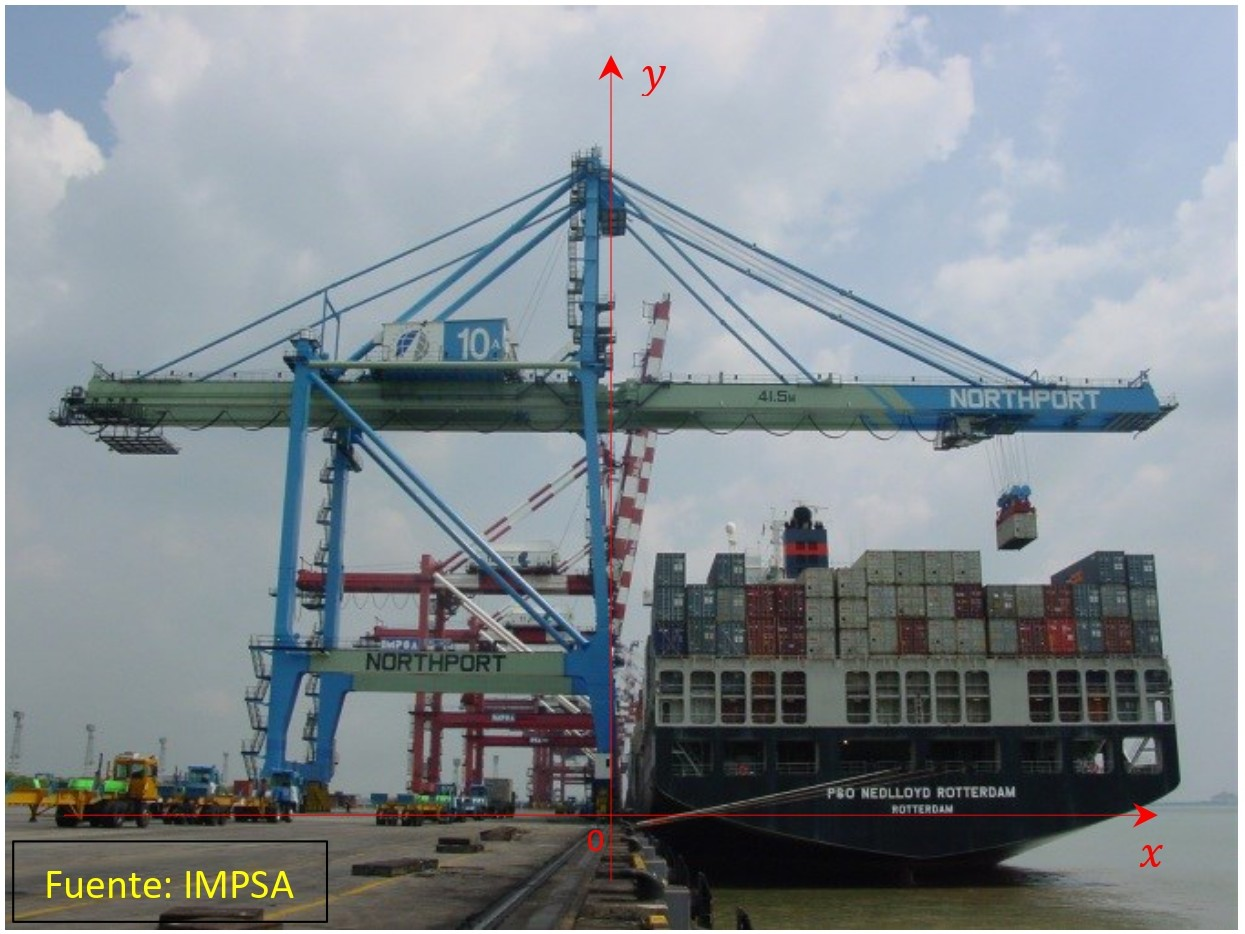
\includegraphics[width=\linewidth]{vista_lateral.jpg}
    \end{column}
  \end{columns}
\end{frame}

\begin{frame}{Arquitectura de control jerárquica}
  \begin{block}{Sistema híbrido de control y protección — 3 niveles}
    \begin{center}
      \begin{tabular}{cll}
        \toprule
        \textbf{Nivel} & \textbf{Rol} & \textbf{Tipo / $T_s$} \\
        \midrule
        \textbf{2} & Regulatorio (torque/velocidad) & Continuo muestreado --- $1$ ms \\
        \textbf{1} & Supervisor (modos, coordinación) & \textbf{Eventos discretos} --- $20$ ms \\
        \textbf{0} & Protección (seguridad) & Eventos discretos --- $20$ ms \\
        \bottomrule
      \end{tabular}
    \end{center}
  \end{block}
  \begin{itemize}
    \item Jerarquía creciente: el Nivel 0 \textbf{sobrescribe} a los superiores ante falla.
    \item La \textbf{planta} (modelo físico y parámetros) es \alert{provista por la cátedra};
          el aporte propio está en el \textbf{diseño de los 3 niveles} y su
          \textbf{implementación}.
  \end{itemize}
\end{frame}

\section{La planta (provista)}

\begin{frame}{Modelo dinámico híbrido de la planta}
  La cátedra entrega el modelo completo. Es \textbf{híbrido}: combina dinámicas continuas con
  cambios discretos de estado.
  \begin{columns}[T]
    \begin{column}{0.5\textwidth}
      \begin{block}{Variables continuas (\textit{flow})}
        \begin{itemize}
          \item Posición/velocidad de carro $x_t,v_t$ e izaje $y_h,v_h$.
          \item Ángulo de balanceo $\theta_l$, tensión de cable $F_{hw}$.
          \item Torques, fuerzas de contacto.
        \end{itemize}
      \end{block}
    \end{column}
    \begin{column}{0.5\textwidth}
      \begin{block}{Estados discretos (\textit{jump})}
        \begin{itemize}
          \item Twistlocks \sig{TLK}: abierto/cerrado.
          \item Contacto: suspendido/apoyado.
          \item Cable: tenso/flojo.
          \item Frenos NC \sig{$BRK$}: abierto/cerrado.
        \end{itemize}
      \end{block}
    \end{column}
  \end{columns}
  \vspace{0.3cm}
  \centering
  \footnotesize Carro e izaje acoplados por la carga pendular; interacción con el perfil de
  obstáculos del entorno.
\end{frame}

\begin{frame}{Implementación de la planta en Simulink}
  \begin{columns}[T]
    \begin{column}{0.62\textwidth}
      \centering
      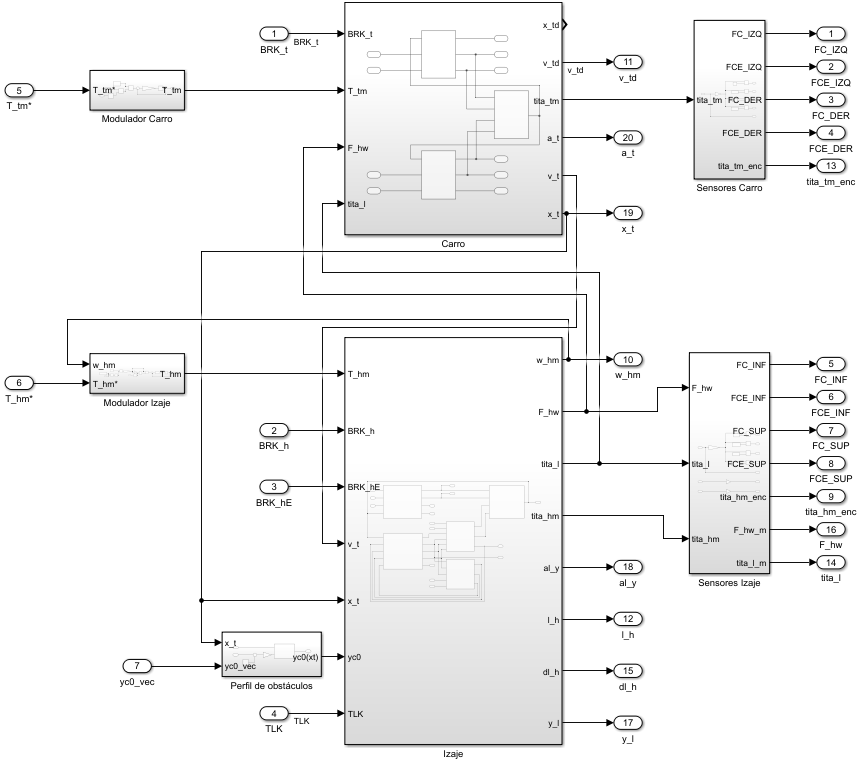
\includegraphics[width=\linewidth]{modelo_planta.png}
    \end{column}
    \begin{column}{0.38\textwidth}
      \footnotesize
      \begin{block}{Parámetros (dados)}
        \begin{tabular}{ll}
          $M_t$ & $30\,000$ kg \\
          $M_s$ & $15\,000$ kg \\
          $M_{c\max}$ & $50\,000$ kg \\
          $i_t / i_h$ & $30 / 22$ \\
          $v_{t\max}$ & $4$ m/s \\
          $v_{h}$ & $1.5$--$3$ m/s \\
        \end{tabular}
      \end{block}
      Sensores: encoders, fines de carrera, celda de carga, ángulo de spreader, LIDAR.
    \end{column}
  \end{columns}
\end{frame}

\begin{frame}{Subsistema del carro: visión general}
  \begin{block}{Función del sistema}
    Traslación horizontal del carro mediante un \textbf{motor} que acciona un \textbf{tambor},
    el cual tira del carro a través de cables de acero.
  \end{block}

  \begin{block}{Modelo: sistema electromecánico de 2 masas}
    \begin{itemize}
      \item \textbf{Masa rotacional}: inercia del accionamiento (motor + tambor + reductor).
      \item \textbf{Masa traslacional}: el carro $M_t$ sobre los rieles.
      \item Acopladas por un \textbf{cable elástico} (resorte-amortiguador).
    \end{itemize}
  \end{block}

  \begin{alertblock}{Hipótesis}
    Transmisión rígida y \textbf{1 cable equivalente} de carro, siempre tensado, con elasticidad
    longitudinal amortiguada.
  \end{alertblock}
\end{frame}

\begin{frame}{Dinámica del carro (2.\textsuperscript{a} ley de Newton)}
  \begin{block}{Movimiento horizontal del carro}
    \[
    M_t \, \frac{dv_t(t)}{dt} = F_{tw}(t) - b_t \, v_t(t) + 2 F_{hw}(t)\sin\theta_l(t)
    \]
  \end{block}

  \vspace{-0.1cm}
  \begin{block}{Términos}
    \begin{itemize}
      \item $F_{tw}(t)$: fuerza de tracción del cable del carro.
      \item $b_t \, v_t(t)$: fricción viscosa sobre los rieles.
      \item $2 F_{hw}(t)\sin\theta_l(t)$: fuerza horizontal por el balanceo de la carga.
    \end{itemize}
    Valores: $M_t = 30\,000$ kg \quad ; \quad $b_t = 90$ Ns/m.
  \end{block}

  \begin{alertblock}{Acoplamiento con el izaje}
    El término $2 F_{hw}\sin\theta_l$ es la \textbf{perturbación del balanceo}: conecta la
    dinámica del carro con la de la carga suspendida.
  \end{alertblock}
\end{frame}

\begin{frame}{Acoplamiento elástico del cable}
  \begin{block}{Modelo resorte-amortiguador}
    El cable transmite la fuerza entre el tambor y el carro:
    \[
    F_{tw}(t) = K_{tw}\,\big(x_{td}(t) - x_t(t)\big) + b_{tw}\,\big(v_{td}(t) - v_t(t)\big)
    \]
  \end{block}

  \begin{block}{Parámetros y variables}
    \begin{itemize}
      \item $K_{tw} = 480 \times 10^3$ N/m \quad (rigidez del cable).
      \item $b_{tw} = 3 \times 10^3$ Ns/m \quad (amortiguamiento).
      \item $x_{td},\,v_{td}$: posición y velocidad lineal \textbf{equivalente del tambor}
            (en su superficie).
    \end{itemize}
  \end{block}

  \begin{alertblock}{Interpretación}
    La fuerza depende de la \textbf{diferencia} tambor--carro: el cable se estira y empuja/tira
    según el desfasaje entre ambos.
  \end{alertblock}
\end{frame}

\begin{frame}{Dinámica del accionamiento: dos ejes}
  \begin{columns}[T]
    \begin{column}{0.4\textwidth}
      \textbf{Eje lento (tambor)}
      \[ J_{td}\,\dot\omega_{td}(t) = T_{td}(t) - b_{td}\,\omega_{td}(t) - T_{tdl}(t) \]
      \begin{itemize}
        \item $J_{td} = 1200$ kgm²
        \item $b_{td} = 1.8$ Nms/rad
        \item $r_{td} = 0.5$ m
        \item $T_{tdl}(t) = F_{tw}(t)\,r_{td}$ (carga del cable)
      \end{itemize}
    \end{column}
    \begin{column}{0.6\textwidth}
      \textbf{Eje rápido (motor)}
      \[ J_{tm+tb}\,\dot\omega_{tm}(t) = T_{tm}(t) + T_{tb}(t,\sig{BRK_t}) - b_{tm}\,\omega_{tm}(t)- T_{tml}(t) \]
      \begin{itemize}
        \item $J_{tm+tb} = 7$ kgm²
        \item $b_{tm} = 6$ Nms/rad
        \item $T_{tm}(t)$: torque del motor
        \item $T_{tb}(t,\sig{BRK_t})$: torque del freno
      \end{itemize}
    \end{column}
  \end{columns}

  \vspace{0.2cm}
  \begin{alertblock}{Unión de los ejes}
    Reductor de relación $i_t = 30$: $\;\omega_{td}\,i_t = \omega_{tm}\;$ y $\;T_{td} = i_t\,T_{tml}$.
  \end{alertblock}
\end{frame}

\begin{frame}{Freno mecánico (Normal Cerrado)}
  \begin{block}{Torque de frenado --- depende de \sig{$BRK_t$}}
    \[
    T_{tb}(\sig{BRK_t}) =
    \begin{cases}
      0 & \sig{BRK_t}=1 \;(\text{abierto}) \\[4pt]
      -T_{tb\max}\tanh(b_{tb}\,\omega_{tm}) & \sig{BRK_t}=0 \;(\text{cerrado})
    \end{cases}
    \]
    \begin{columns}[c]
      \begin{column}{0.42\textwidth}
        \begin{itemize}
          \item $T_{tb\max} = 5 \times 10^3$ Nm
          \item $b_{tb} = 5 \times 10^6$ Nms/rad
        \end{itemize}
      \end{column}
      \begin{column}{0.48\textwidth}
        \centering
        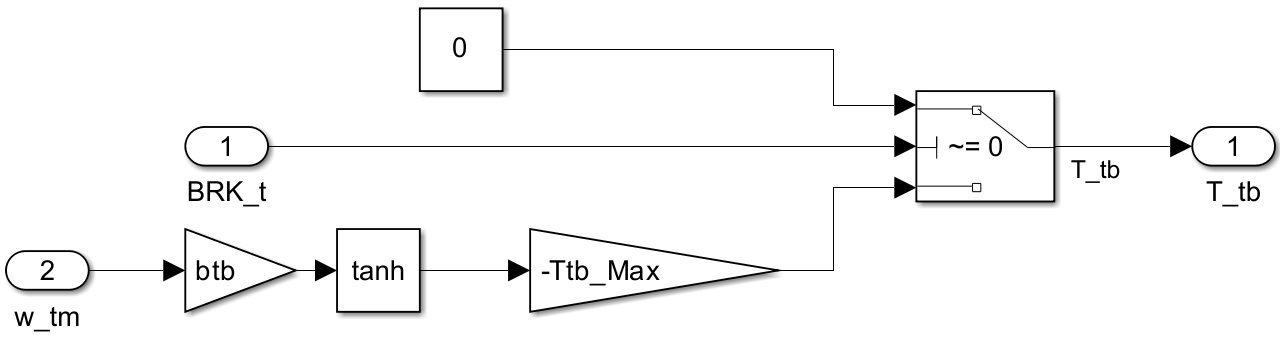
\includegraphics[width=\linewidth]{freno_carro.png}
      \end{column}
    \end{columns}
  \end{block}

  \begin{alertblock}{Por qué $\tanh$}
    Función continua y abrupta: frena fuerte pero evita la \textbf{discontinuidad numérica}
    del signo en la simulación.
  \end{alertblock}
\end{frame}

\begin{frame}{Modelo equivalente referido al motor}
  \begin{block}{Reducción a un solo eje}
    Se refiere la dinámica del tambor al eje del motor usando $i_t = 30$, agrupando inercias y
    fricciones:
  \end{block}

  \vspace{-0.2cm}
  \[
  J_{t,eq} = J_{tm+tb} + \frac{J_{td}}{i_t^2} = 7 + \frac{1200}{30^2} \approx 8.33 \text{ kgm}^2
  \]
  \vspace{-0.2cm}
  \[
  b_{t,eq} = b_{tm} + \frac{b_{td}}{i_t^2} = 6 + \frac{1.8}{30^2} \approx 6.002 \text{ Nms/rad}
  \]

  \begin{alertblock}{Resultado}
    Ecuación de estado única para todo el accionamiento del carro:
    \[
    \frac{d\omega_{tm}}{dt}(t) = \frac{1}{J_{t,eq}}\left[T_{tm}(t) + T_{tb}(t,\sig{BRK_t}) - b_{t,eq}\,\omega_{tm}(t)
      - \frac{r_{td}}{i_t}F_{tw}(t)\right]
    \]
  \end{alertblock}
\end{frame}

\begin{frame}{Modelo dinámico completo del carro}
  \vspace{-0.2cm}
  \begin{columns}[T]
    \begin{column}{0.65\textwidth}
      \begin{block}{Ecuaciones de estado acopladas}
        \[
        \begin{cases}
          \dot\omega_{tm}(t) = \frac{1}{J_{t,eq}}\big[T_{tm}(t) + T_{tb}(t,\sig{BRK_t}) - b_{t,eq}\,\omega_{tm}(t)
            - \tfrac{r_{td}}{i_t}F_{tw}(t)\big] \\[6pt]
          \dot v_t(t) = \frac{1}{M_t}\big[F_{tw}(t) - b_t\,v_t(t) + 2F_{hw}(t)\sin\theta_l(t)\big] \\[6pt]
          \dot x_t(t) = v_t(t) \\[6pt]
          F_{tw}(t) = K_{tw}\big(x_{td}(t)-x_t(t)\big) + b_{tw}\big(v_{td}(t)-v_t(t)\big)
        \end{cases}
        \]
      \end{block}
      \begin{block}{Variables auxiliares}
        $v_{td}(t) = \dfrac{r_{td}}{i_t}\,\omega_{tm}(t)$ \quad ; \quad $x_{td}(t) = \displaystyle\int v_{td}(t)\,dt$
      \end{block}
    \end{column}
    \begin{column}{0.35\textwidth}
      \centering
      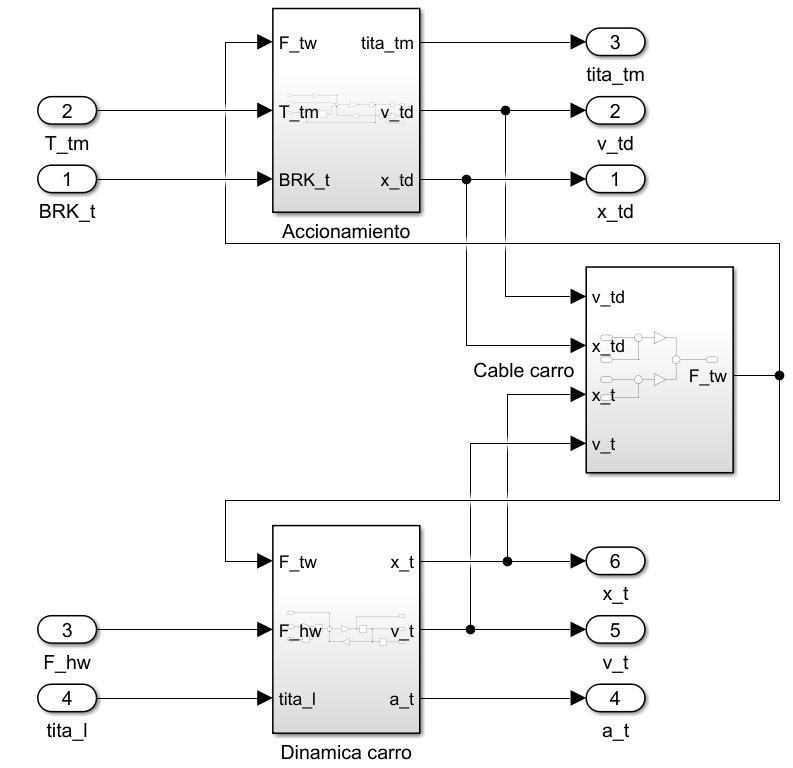
\includegraphics[width=\linewidth]{modelo_carro.png}
    \end{column}
  \end{columns}

  % \vspace{-0.2cm}
  \begin{alertblock}{Dimensionalidad}
    \textbf{3 estados continuos} ($\omega_{tm}, v_t, x_t$) + el \textbf{freno} como evento discreto
    (\sig{$BRK_t$}).
  \end{alertblock}
\end{frame}

% \lautimode
\begin{frame}{Subsistema de izaje}
  \begin{block}{Características del sistema}
    Controla la elevación de la carga mediante:
    \begin{itemize}
      \item Motor eléctrico accionando un \textbf{tambor}
      \item Sistema de cableado con relación de transmisión \textbf{2:1} (aparejo móvil)
      \item Carga suspendida: \textbf{2 grados de libertad}
    \end{itemize}
    Característica clave:
    \begin{itemize}
    \item\alert{Dinámica híbrida}
    \end{itemize}
  \end{block}
\end{frame}

\begin{frame}{Parámetros discretos}
  \begin{block}{Masa total ($m_l$)}
    \[
    m_l(\text{TLK}) = 
    \begin{cases} 
      M_s & \text{si TLK} = 0 \text{ (solo spreader)} \\[6pt]
      M_s + M_{cX} & \text{si TLK} = 1 \text{ (spreader + contenedor)}
    \end{cases}
    \]
  \end{block}

  \begin{block}{Altura de la carga ($h_c$)}
    \[
    h_c(\text{TLK}) = 
    \begin{cases} 
      0 & \text{si TLK} = 0 \\
      H_c & \text{si TLK} = 1
    \end{cases}
    \]
  \end{block}
\end{frame}

\begin{frame}{Ecuaciones de movimiento de la carga}
  \begin{block}{Dinámicas acopladas}
    \begin{equation*}
      m_l(\textcolor{signalcolor}{TLK}) \, \frac{d \, v_{lx}(t)}{dt} = -2 F_{hw}(t,l(t)-l_h(t)) \, \sin\theta_l(t) + F_{cx}(t, \delta y)
    \end{equation*}
    \begin{equation*}
        m_l(\textcolor{signalcolor}{TLK}) \, \frac{d \, v_{ly}(t)}{dt} = 2 F_{hw}(t,l(t)-l_h(t)) \, \cos\theta_l(t) - m_l(\textcolor{signalcolor}{TLK}) \, g + F_{cy}(t, \delta y)
    \end{equation*}
    \begin{equation*}
      \delta y = y_l(t) - h_c(\textcolor{signalcolor}{TLK}) - y_{c0}(x_l(t), t)
    \end{equation*}
  \end{block}
\end{frame}

\begin{frame}{Interacción con el entorno}
  \begin{block}{Condición de contacto}
    Cuando: $\delta y \le 0$ 
  \end{block}

  \begin{block}{Fuerza vertical}
    \[
    F_{cy} = 
    \begin{cases} 
      K_{cy}(y_{c0} - (y_l - h_c)) - b_{cy} v_{ly} & \text{(Apoyado)} \\[4pt]
      0 & \text{(Suspendido)}
    \end{cases}
    \]
  \end{block}

  \begin{block}{Fuerza horizontal}
    \[
    F_{cx} = 
    \begin{cases} 
      -b_{cx} v_{lx} & \text{(Apoyado)} \\[4pt]
      0 & \text{(Suspendido)}
    \end{cases}
    \]
  \end{block}
\end{frame}

\begin{frame}{Acoplamiento elástico del cable}
  \begin{block}{Resorte-amortiguador con rigidez variable}
    La rigidez y amortiguamiento escalan con la longitud del cable bajo tensión:
    \[
    K_{hw}(l_h) = \frac{k_{hwu}}{2 l_h + L_{h0}} \quad ; \quad b_{hw}(l_h) = b_{hwu}(2 l_h + L_{h0})
    \]
  \end{block}

  \begin{block}{Fuerza de tensión}
    \[
    F_{hw} = 
    \begin{cases} 
      K_{hw}(l_h) \cdot 2(l - l_h) + b_{hw}(l_h) \cdot 2(\dot{l} - \dot{l}_h) & \text{(Tenso)} \\[4pt]
      0 & \text{(Flojo)}
    \end{cases}
    \]
  \end{block}
\end{frame}

\begin{frame}{Dinámica del accionamiento}
  \small
  \begin{block}{Ecuaciones de  los dos ejes}
    \begin{itemize}
      \item \textbf{Eje lento(tambor):}
      \begin{equation*}
        J_{hd+hEb} \, \frac{d \, \omega_{hd}(t)}{dt} = T_{hd}(t) + T_{hEb}(t,\textcolor{signalcolor}{BRK_{hE}}) - b_{hd} \, \omega_{hd}(t) - T_{hdl}(t)
      \end{equation*}
      \item \textbf{Eje rápido(motor):} 
      \begin{equation*}
        J_{hm+hb} \, \frac{d \, \omega_{hm}(t)}{dt} = T_{hm}(t) + T_{hb}(t,\textcolor{signalcolor}{BRK_{h}}) - b_{hm} \, \omega_{hm}(t) - T_{hml}(t)
      \end{equation*}
    \end{itemize}
  \end{block}

  \vspace{0.2cm}
  \begin{block}{Relación cinemática}
    \[
    v_h(t) = \frac{r_{hd} \omega_{hd}(t)}{2} = -\frac{dl_h}{dt}
    \]
    Factor 2 divide la velocidad tangencial del tambor
  \end{block}
\end{frame}

\begin{frame}{Frenos mecánicos}
\begin{figure}
  \centering
  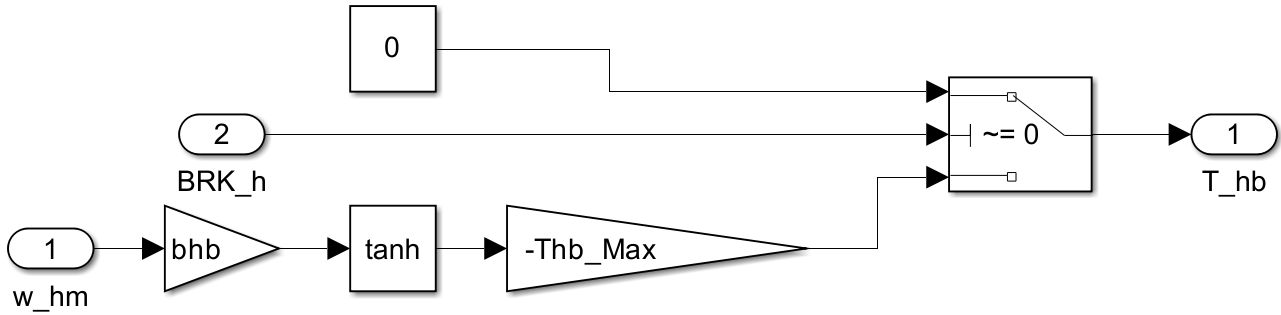
\includegraphics[width=0.8\textwidth]{freno_izaje.png}
  \caption{Freno mecánico de operación izaje}
\end{figure}
\begin{figure}
  \centering
  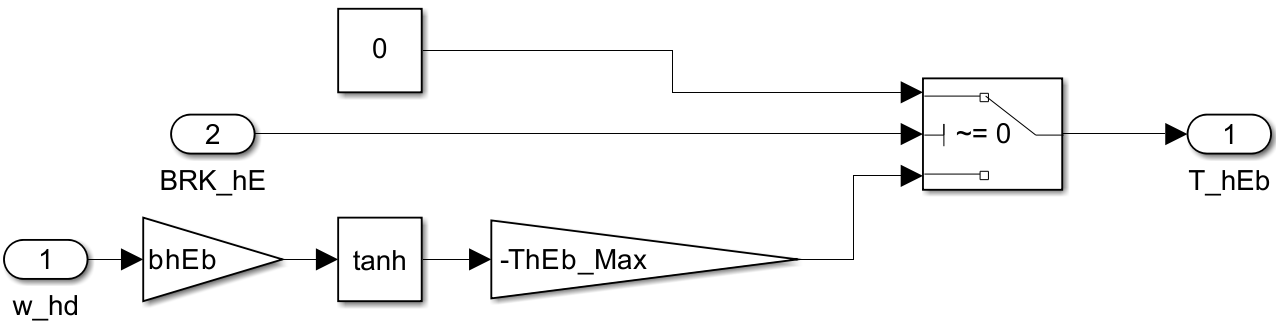
\includegraphics[width=0.8\textwidth]{freno_izaje_e.png}
  \caption{Freno mecánico de emergencia izaje}
\end{figure}
\end{frame}

\begin{frame}{Modelo equivalente referido al motor}
  \begin{block}{Reducción eje equivalente}
    Al igual que el carro, se refiere la dinámica del tambor al motor usando $i_h$:
  \end{block}

  \vspace{-0.2cm}
  \[
  J_{h,eq} = J_{hm+hb} + \frac{J_{hd+hEb}}{i_h^2}
  \]

  \vspace{-0.3cm}
  \[
  b_{h,eq} = b_{hm} + \frac{b_{hd}}{i_h^2} 
  \]
  \begin{block}{Variables auxiliares}
    \vspace{-0.2cm}
    \begin{itemize}
      \item Longitud geométrica: $l(t) = \sqrt{(x_l - x_t)^2 + (Y_{t0} - y_l)^2}$
      \item Velocidad de cambio: $\frac{dl}{dt} = \frac{(x_l - x_t)(v_{lx} - v_t) - (Y_{t0} - y_l)v_{ly}}{l}$
      \item Ángulo de balanceo: $\theta_l = \text{atan2}\left(\frac{x_l - x_t}{Y_{t0} - y_l}\right)$
    \end{itemize}
  \end{block}
\end{frame}

\begin{frame}{Subsistema izaje completo}
\begin{figure}
  \centering
  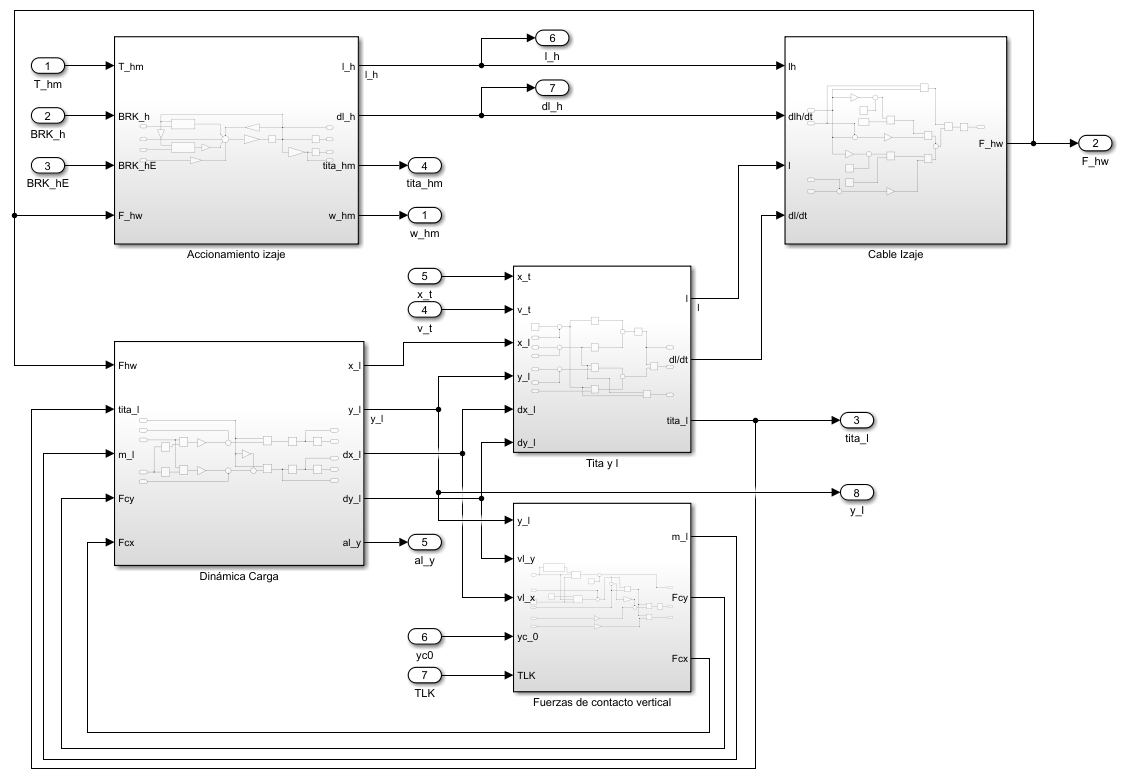
\includegraphics[width=0.77\textwidth]{modelo_izaje.png}
  %\caption{Diagrama de bloques del subsistema de izaje}
\end{figure}
  
\end{frame}

\begin{frame}{Sensores}
  \begin{block}{Sensor carro}
    \begin{itemize}
    \item \textbf{Encoder:} Mide la posición angular del motor del carro $\theta_{tm}(t)$
    \[
  x_t(t) = \theta_{tm}(t) \, \frac{r_{tm}}{i_t}
    \]
    \end{itemize}
  \end{block}
  \begin{block}{Sensores izaje}
    \begin{itemize}
    \item \textbf{Encoder:} Mide posición angular del motor de izaje $\theta_{hm}(t)$
    \[
    y_h(t) = \theta_{hm}(t) \, \frac{r_{hd}}{2\,i_h}
    \]
    \item \textbf{Celda de carga:} Mide fuerza de tensión $F_{hw}(t)$ en el cable de izaje
    \item \textbf{Sensor de ángulo de spreader:} Mide ángulo de balanceo $\theta_l(t)$ y velocidad angular $\dot{\theta}_l(t)$ 
    de la carga suspendida
    \end{itemize}
  \end{block}
\end{frame}

\begin{frame}{Fines de carrera}
  \begin{block}{FC del carro}
    \vspace{0.2cm}
    \begin{columns}[T]
      \begin{column}{0.5\textwidth}
        \[
        \text{FC}_{t,\text{der}} = 
        \begin{cases} 
          0 & \text{si } x_t < x_{t\max} \\[4pt]
          1 & \text{si } x_t \ge x_{t\max} \\[4pt]
          1 & \text{si } x_t \ge x_{t\max} + 0.5 \text{ m (E)}
        \end{cases}
        \]
      \end{column}
      \begin{column}{0.5\textwidth}
        \[
        \text{FC}_{t,\text{izq}} = 
        \begin{cases} 
          0 & \text{si } x_t > x_{t\min} \\
          1 & \text{si } x_t \le x_{t\min} \\[4pt]
          1 & \text{si } x_t \le x_{t\min} + 0.5 \text{ m (E)}
        \end{cases}
        \]
      \end{column}
    \end{columns}
  \end{block}
    \begin{block}{FC del izaje}
    \vspace{0.2cm}
    \begin{columns}[T]
      \begin{column}{0.5\textwidth}
        \[
        \text{FC}_{h,\text{sup}} = 
        \begin{cases} 
          0 & \text{si } y_h < y_{h\max} \\[4pt]
          1 & \text{si } y_h \ge y_{h\max} \\[4pt]
          1 & \text{si } y_h \ge y_{h\max} + 0.5 \text{ m (E)}
        \end{cases}
        \]
      \end{column}
      \begin{column}{0.5\textwidth}
        \[
        \text{FC}_{h,\text{inf}} = 
        \begin{cases} 
          0 & \text{si } y_h > y_{h\min} \\[4pt]
          1 & \text{si } y_h \le y_{h\min}  \\[4pt]
          1 & \text{si } y_h \le y_{h\min} + 0.5 \text{ m (E)}
        \end{cases}
        \]
      \end{column}
    \end{columns}
  \end{block}
\end{frame}



\begin{frame}{Modelo sensores}
  \begin{columns}[T]
    \begin{column}{0.48\textwidth}
      \vspace{1cm}
      \centering
      \begin{figure}
      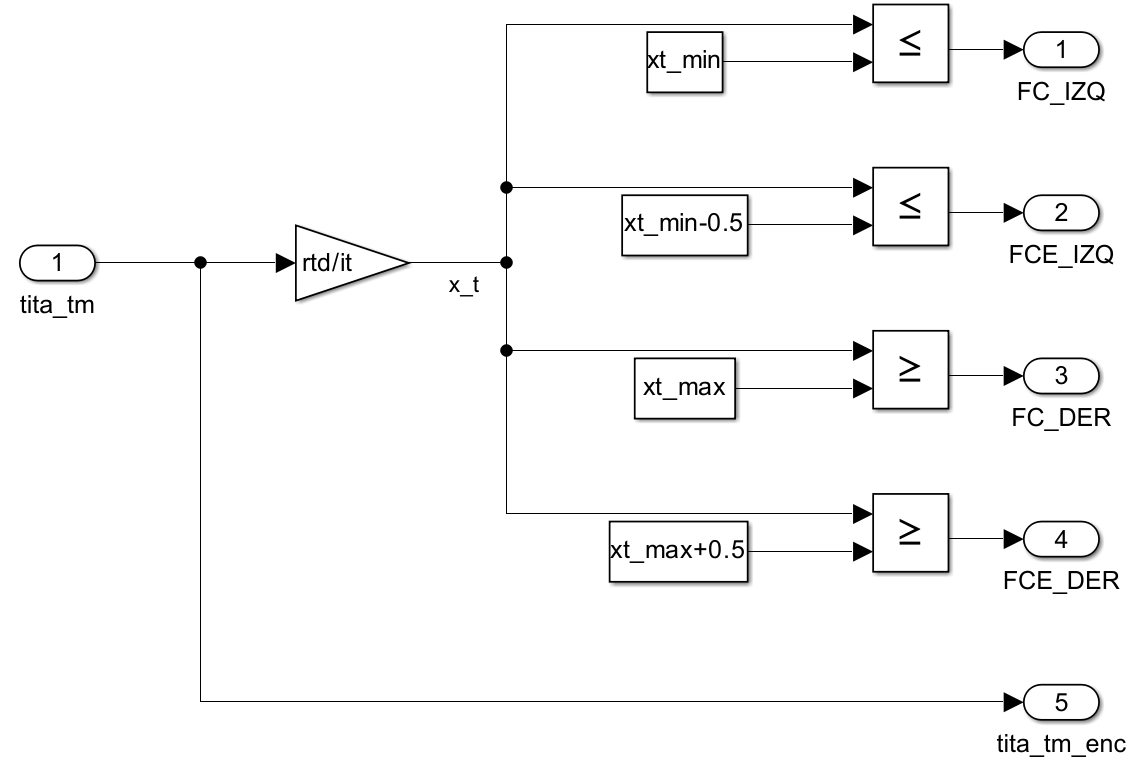
\includegraphics[width=\textwidth]{sensores_carro.png}
      \caption{Diagrama de bloques sensores carro e izaje Simulink}
      \end{figure}
    \end{column}
    \begin{column}{0.48\textwidth}
      \centering
      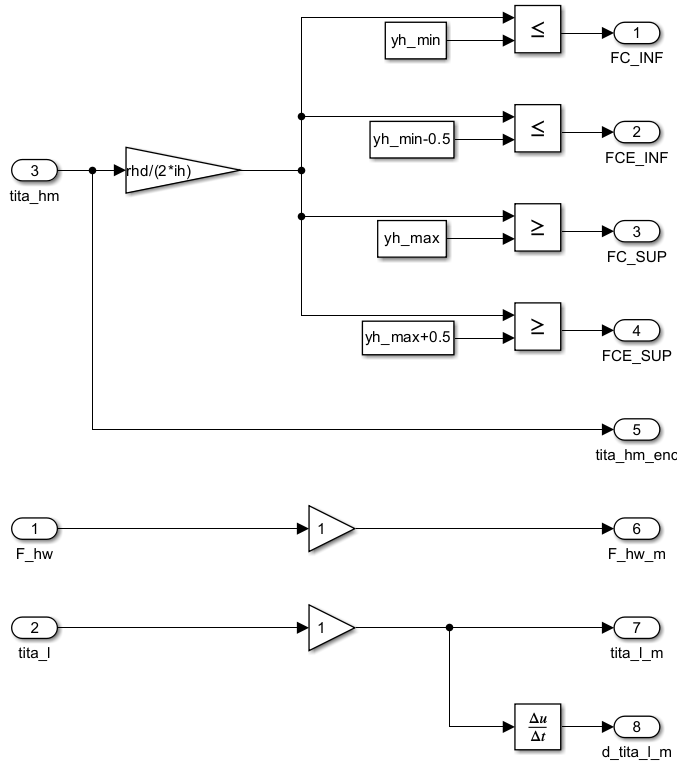
\includegraphics[width=\textwidth]{sensores_izaje.png}
    \end{column}
  \end{columns}
\end{frame}


\begin{frame}{Moduladores de torque}
  \begin{block}{Función en la simulación}
    Modelan las limitaciones de los \textbf{accionamientos reales} (motores eléctricos)
    \begin{itemize}
      \item No es posible aplicar torque instantáneo como una fuerza mecánica ideal
      \item Los motores reales tienen capacidad limitada y retardo dinámico
    \end{itemize}
  \end{block}

  \begin{block}{Dos funciones clave}
    \begin{enumerate}
      \item \textbf{Saturación}: limita torque a máximo permitido $T_{\max}$
      \item \textbf{Filtrado}: modela retardo electromagnético con constante $\tau = 1$ ms
    \end{enumerate}
  \end{block}
  \begin{block}{Ecuación diferencial}
    Vincula el torque limitado comandado $T_{\text{Lim}}^*(t)$ con el torque físico real $T(t)$:
    \vspace{-0.2cm}
    \[
    \tau \frac{dT(t)}{dt} = T_{\text{Lim}}^*(t) - T(t)
    \]
  \end{block}

\end{frame}


\begin{frame}{Modulador del carro}
  \begin{block}{Ecuación}
    \[
T_{tm\ Lim}^*(k \, T_{s2} \leq t < (k+1) \, T_{s2}) = \text{min}\left(+T_{tm\max}, \text{max}\left(-T_{tm\max}, T_{tm}^*(k \, T_{s2})\right)\right)
    \]
  \end{block}
  \begin{figure}
  \centering
  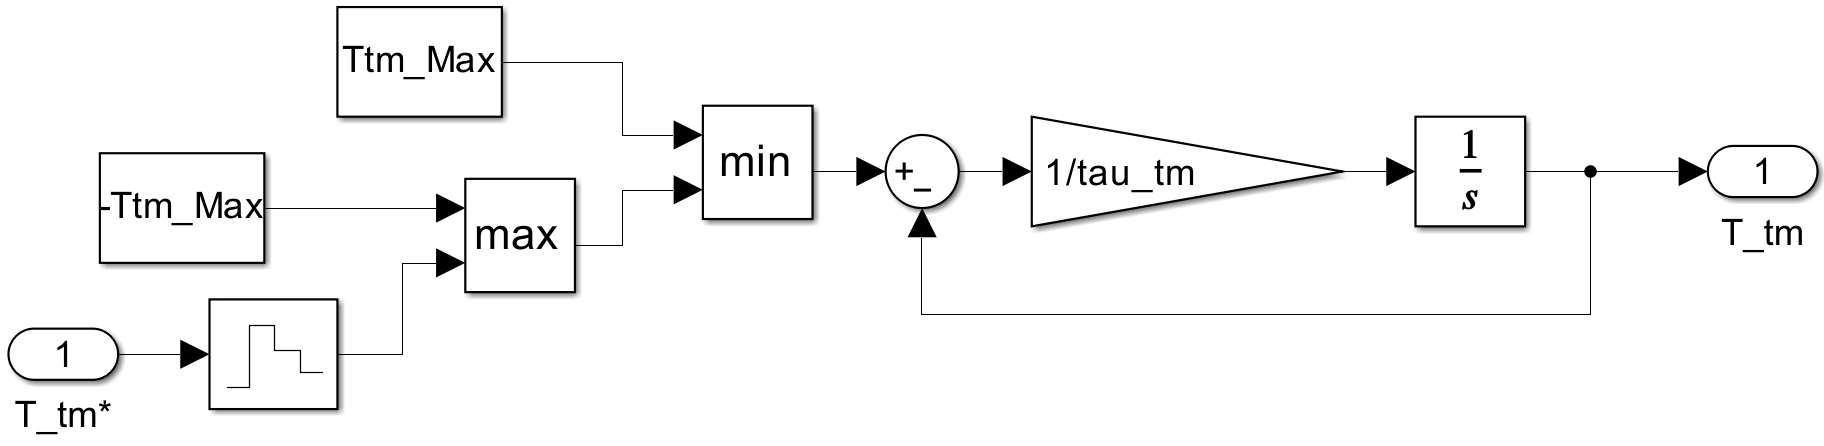
\includegraphics[width=1\textwidth]{modulador_carro.png}
  \caption{Diagrama de bloques del modulador de torque del carro}
  \end{figure}
\end{frame}


% \defaultmode
\begin{frame}{Discretización del perfil de obstáculos}
  \begin{columns}[T]
    \begin{column}{0.55\textwidth}
      \begin{block}{Relevamiento por LIDAR}
        El LIDAR del carro releva el \textbf{perfil de obstáculos} $y_{c0}(x,t)$ (pila de
        contenedores, muelle, barco).
      \end{block}

      \begin{block}{Discretización por ancho de contenedor}
        Paso $= W_c = 2.44$ m (contenedor ISO):
        \[
        N_{x_t} = \left\lfloor \frac{x_{t\max}-x_{t\min}}{W_c} \right\rfloor + 1
                = \left\lfloor \frac{80}{2.44} \right\rfloor + 1 = 33
        \]
        Índices $i = 1,\dots,33$.
      \end{block}
    \end{column}
    \begin{column}{0.45\textwidth}
      \centering
      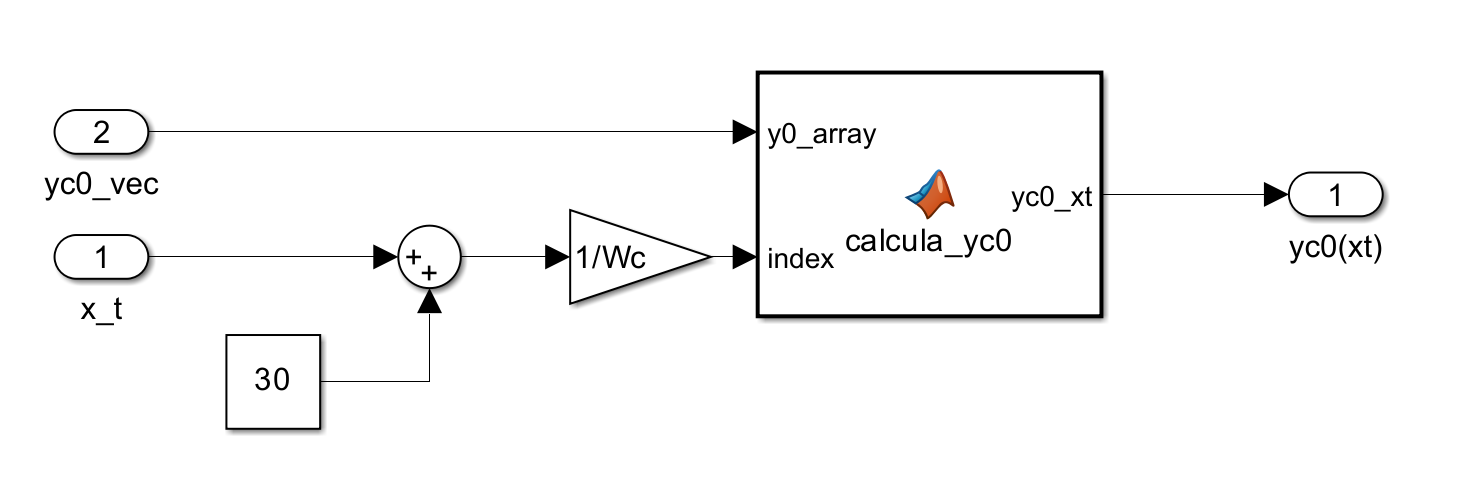
\includegraphics[width=\linewidth]{perfil_obstaculos.png}
    \end{column}
  \end{columns}

  \begin{alertblock}{Vector de perfil $y_{c0\,vec}$}
    Vector de $33$ alturas conocido por el autómata; se \textbf{actualiza} al mover contenedores.
    El modo automático exige el perfil \textbf{escaneado por completo}.
  \end{alertblock}
\end{frame}

% \lautimode

\begin{frame}{Sensores}
  \begin{block}{Sensor carro}
    \begin{itemize}
    \item \textbf{Encoder:} Mide la posición angular del motor del carro $\theta_{tm}(t)$
    \[
  x_t(t) = \theta_{tm}(t) \, \frac{r_{tm}}{i_t}
    \]
    \end{itemize}
  \end{block}
  \begin{block}{Sensores izaje}
    \begin{itemize}
    \item \textbf{Encoder:} Mide posición angular del motor de izaje $\theta_{hm}(t)$
    \[
    y_h(t) = \theta_{hm}(t) \, \frac{r_{hd}}{2\,i_h}
    \]
    \item \textbf{Celda de carga:} Mide fuerza de tensión $F_{hw}(t)$ en el cable de izaje
    \item \textbf{Sensor de ángulo de spreader:} Mide ángulo de balanceo $\theta_l(t)$ y velocidad angular $\dot{\theta}_l(t)$ 
    de la carga suspendida
    \end{itemize}
  \end{block}
\end{frame}

\begin{frame}{Fines de carrera}
  \begin{block}{FC del carro}
    \vspace{0.2cm}
    \begin{columns}[T]
      \begin{column}{0.5\textwidth}
        \[
        \text{FC}_{t,\text{der}} = 
        \begin{cases} 
          0 & \text{si } x_t < x_{t\max} \\[4pt]
          1 & \text{si } x_t \ge x_{t\max} \\[4pt]
          1 & \text{si } x_t \ge x_{t\max} + 0.5 \text{ m (E)}
        \end{cases}
        \]
      \end{column}
      \begin{column}{0.5\textwidth}
        \[
        \text{FC}_{t,\text{izq}} = 
        \begin{cases} 
          0 & \text{si } x_t > x_{t\min} \\
          1 & \text{si } x_t \le x_{t\min} \\[4pt]
          1 & \text{si } x_t \le x_{t\min} + 0.5 \text{ m (E)}
        \end{cases}
        \]
      \end{column}
    \end{columns}
  \end{block}
    \begin{block}{FC del izaje}
    \vspace{0.2cm}
    \begin{columns}[T]
      \begin{column}{0.5\textwidth}
        \[
        \text{FC}_{h,\text{sup}} = 
        \begin{cases} 
          0 & \text{si } y_h < y_{h\max} \\[4pt]
          1 & \text{si } y_h \ge y_{h\max} \\[4pt]
          1 & \text{si } y_h \ge y_{h\max} + 0.5 \text{ m (E)}
        \end{cases}
        \]
      \end{column}
      \begin{column}{0.5\textwidth}
        \[
        \text{FC}_{h,\text{inf}} = 
        \begin{cases} 
          0 & \text{si } y_h > y_{h\min} \\[4pt]
          1 & \text{si } y_h \le y_{h\min}  \\[4pt]
          1 & \text{si } y_h \le y_{h\min} + 0.5 \text{ m (E)}
        \end{cases}
        \]
      \end{column}
    \end{columns}
  \end{block}
\end{frame}



\begin{frame}{Modelo sensores}
  \begin{columns}[T]
    \begin{column}{0.48\textwidth}
      \vspace{1cm}
      \centering
      \begin{figure}
      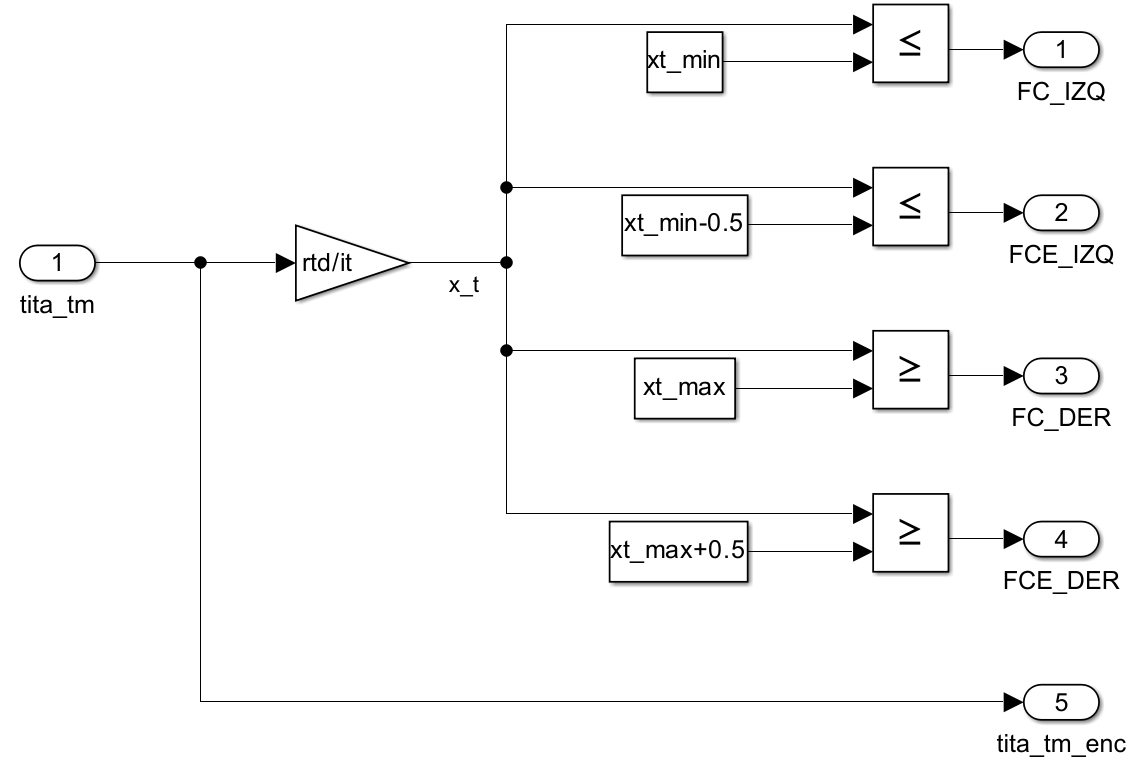
\includegraphics[width=\textwidth]{sensores_carro.png}
      \caption{Diagrama de bloques sensores carro e izaje Simulink}
      \end{figure}
    \end{column}
    \begin{column}{0.48\textwidth}
      \centering
      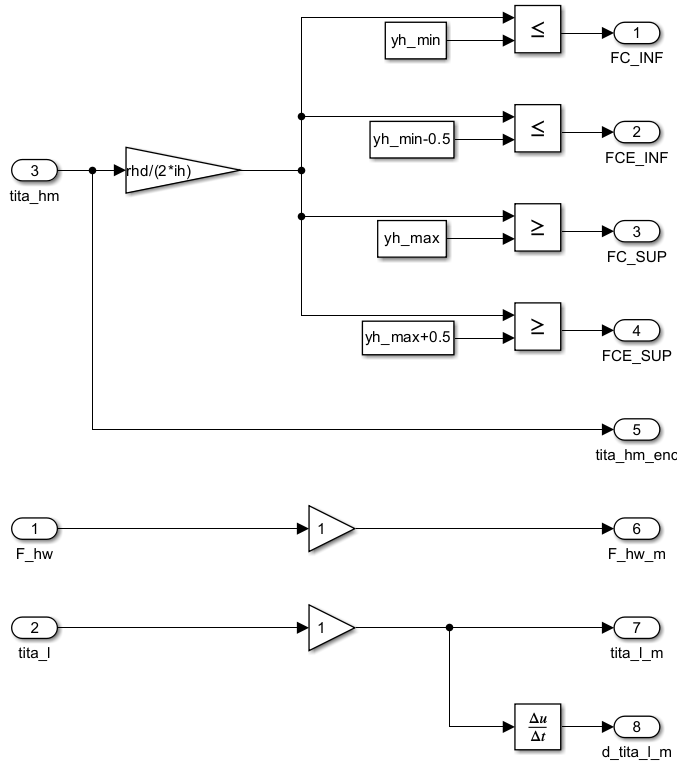
\includegraphics[width=\textwidth]{sensores_izaje.png}
    \end{column}
  \end{columns}
\end{frame}


\begin{frame}{Moduladores de torque}
  \begin{block}{Función en la simulación}
    Modelan las limitaciones de los \textbf{accionamientos reales} (motores eléctricos)
    \begin{itemize}
      \item No es posible aplicar torque instantáneo como una fuerza mecánica ideal
      \item Los motores reales tienen capacidad limitada y retardo dinámico
    \end{itemize}
  \end{block}

  \begin{block}{Dos funciones clave}
    \begin{enumerate}
      \item \textbf{Saturación}: limita torque a máximo permitido $T_{\max}$
      \item \textbf{Filtrado}: modela retardo electromagnético con constante $\tau = 1$ ms
    \end{enumerate}
  \end{block}
  \begin{block}{Ecuación diferencial}
    Vincula el torque limitado comandado $T_{\text{Lim}}^*(t)$ con el torque físico real $T(t)$:
    \vspace{-0.2cm}
    \[
    \tau \frac{dT(t)}{dt} = T_{\text{Lim}}^*(t) - T(t)
    \]
  \end{block}

\end{frame}


\begin{frame}{Modulador del carro}
  \begin{block}{Ecuación}
    \[
T_{tm\ Lim}^*(k \, T_{s2} \leq t < (k+1) \, T_{s2}) = \text{min}\left(+T_{tm\max}, \text{max}\left(-T_{tm\max}, T_{tm}^*(k \, T_{s2})\right)\right)
    \]
  \end{block}
  \begin{figure}
  \centering
  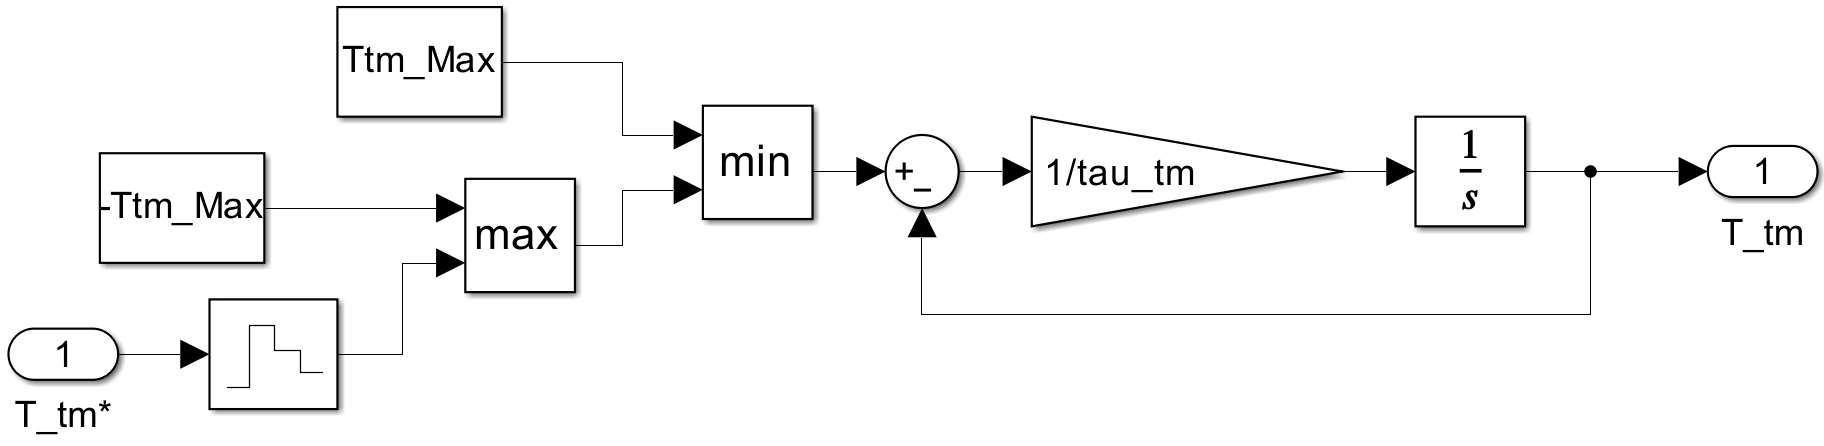
\includegraphics[width=1\textwidth]{modulador_carro.png}
  \caption{Diagrama de bloques del modulador de torque del carro}
  \end{figure}
\end{frame}

% \defaultmode
\begin{frame}{Modulador de torque del izaje}
  \begin{block}{Límite de torque variable con la velocidad}
    A diferencia del carro, el torque máximo se \textbf{reduce a alta velocidad}
    (\textbf{debilitamiento de campo}, potencia constante):
    \[
    T_{hm\max}(t) = T_{hm\,MAX}\,\min\!\left(1,\left(\frac{\omega_{hm\,RATED}}{\omega_{hm}(t)}\right)^2\right)
    \]
    \centering
    $T_{hm\,MAX} = 20 \times 10^3$ Nm \quad ; \quad
    $\omega_{hm\,RATED} = \dfrac{2\,v_{h\,nom}\,i_h}{r_{hd}} = 88$ rad/s
  \end{block}

  \vspace{-0.15cm}
  \begin{block}{Saturación y filtro}
    $T_{hm\,Lim}^*(k) = \operatorname{sat}\!\big(T_{hm}^*(k),\ \pm T_{hm\max}(t)\big)$;\quad
    filtro de 1.\textsuperscript{er} orden ($\tau = 1$ ms) y ZOH, igual que el carro.
  \end{block}

  \vspace{-0.1cm}
  \centering
  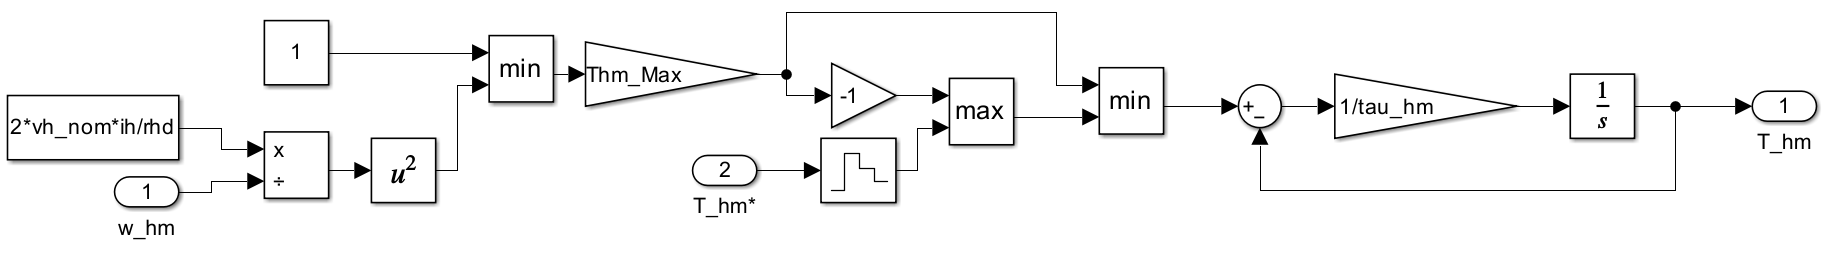
\includegraphics[width=0.72\linewidth]{modulador_izaje.png}
\end{frame}

% \lautimode
\section{Nivel 2 --- Control regulatorio}
\begin{frame}{Nivel 2: objetivo}
  \begin{block}{Función del control regulatorio}
    Genera comandos de \textbf{torque} $T_{tm}^*$ a partir de referencias de \textbf{velocidad} $v_t^*$ provenientes del Nivel 1 (supervisor)
  \end{block}

  \begin{block}{Objetivos de control}
    \begin{itemize}
      \item Seguimiento preciso de referencias de velocidad
      \item Suavidad en la respuesta transitoria
      \item Atenuación de perturbaciones: balanceo de carga, variaciones de masa
      \item Operación en tiempo discretizado (muestreado)
    \end{itemize}
  \end{block}

  \vspace{0.2cm}
  \begin{alertblock}{Estrategia de control}
    \textbf{Lazo regulador PI} + \textbf{compensaciones} (anti-windup) para mejorar respuesta ante saturación y frenos
  \end{alertblock}
\end{frame}

\begin{frame}{Modelo del carro para control de velocidad}
  \begin{block}{Dinámica simplificada de traslación}
    Se desprecian dinámicas rotacionales internas del accionamiento y se agrupan perturbaciones externas:
    \[
    M_t\,\frac{dv_t(t)}{dt} + b_t\,v_t(t) = F_{\text{cmd}}(t) + F_{\text{pert}}(t)
    \]
  \end{block}

  \vspace{-0.2cm}
  \begin{block}{Términos de la ecuación}
    \begin{itemize}
      \item $F_{\text{cmd}}(t) = K_f \, T_{tm}(t)$ con $K_f = \frac{i_t}{r_{td}}$ (conversión torque → fuerza)
      \vspace{0.05cm}
      \item $F_{\text{pert}}(t) = 2F_{hw}(t)\sin(\theta_l(t)) + T_{tb}(t,\text{BRK}_t) K_f$ 
      \begin{itemize}
        \item Componente horizontal del cable (acoplamiento)
        \item Fricción del freno de operación
      \end{itemize}
    \end{itemize}
  \end{block}

  \begin{alertblock}{Aproximación para diseño}
    Se descuida la fricción viscosa $b_t$ frente a la inercia dominante:
    \[
    G_{vel,t}(s) \approx \frac{K_f}{M_t\,s}
    \]
  \end{alertblock}
\end{frame}

\begin{frame}{Función de transferencia completa}
  \begin{block}{Planta sin aproximación}
    \[
    G_{vel,t}(s) = \frac{V_t(s)}{T_{tm}(s)} = \frac{K_f}{M_t\,s + b_t}
    \]
    con polo mecánico $P_{\text{mec}} = -\frac{b_t}{M_t}$ (pequeño en magnitud)
  \end{block}

  \vspace{-0.1cm}
  \begin{block}{Transformada de Laplace}
    Aplicando a la ecuación del carro:
    \[
    M_t\,s\,V_t(s) + b_t\,V_t(s) = K_f\,T_{tm}(s) + F_{\text{pert}}(s)
    \]
    Despejando $V_t(s)$:
    \[
    V_t(s) = \frac{K_f}{M_t\,s + b_t} \, T_{tm}(s) + \frac{1}{M_t\,s + b_t} \, F_{\text{pert}}(s)
    \]
  \end{block}

  \begin{alertblock}{Justificación de la aproximación}
    Como $b_t \ll M_t \, \omega_n$, el polo en $-b_t/M_t$ está muy alejado del eje jw. Se desprecia para simplificar el diseño.
  \end{alertblock}
\end{frame}

\begin{frame}{Diseño del controlador PI: especificación}
  \begin{block}{Tipo de controlador}
    Proporcional-integral (PI):
    \[
    C_{\text{vel}}(s) = K_p + \frac{K_i}{s}
    \]
  \end{block}

  \vspace{-0.1cm}
  \begin{block}{Beneficios del PI}
    \begin{itemize}
      \item Error nulo ante escalones de referencia de velocidad
      \item Buen rechazo de perturbaciones constantes (gravedad, fricción estática)
      \item Estructura simple, fácil de sintonizar
    \end{itemize}
  \end{block}

  \vspace{0.1cm}
  \begin{block}{Función de transferencia a lazo cerrado}
    \[
    T(s) = \frac{C_{\text{vel}}(s) \, G_{vel,t}(s)}{1 + C_{\text{vel}}(s) \, G_{vel,t}(s)} = \frac{K_p K_f\,s + K_i K_f}{M_t\,s^2 + K_p K_f\,s + K_i K_f}
    \]
  \end{block}
\end{frame}

\begin{frame}{Asignación de polos: ecuación característica}
  \begin{block}{Polinomio característico deseado de 2do orden}
    \[
    s^2 + 2\zeta\omega_n\,s + \omega_n^2
    \]
    con amortiguamiento $\zeta$ y frecuencia natural $\omega_n$
  \end{block}

  \vspace{-0.1cm}
  \begin{block}{Ecuación característica del lazo cerrado}
    \[
    M_t\,s^2 + K_p K_f\,s + K_i K_f = 0
    \]
    Dividiendo por $M_t$:
    \[
    s^2 + \frac{K_p K_f}{M_t}\,s + \frac{K_i K_f}{M_t} = 0
    \]
  \end{block}

  \vspace{-0.1cm}
  \begin{block}{Comparación e igualación de coeficientes}
    \begin{align*}
      \frac{K_p K_f}{M_t} &= 2\zeta\omega_n \quad \Rightarrow \quad K_p = \frac{2\zeta\omega_n M_t}{K_f} \\[4pt]
      \frac{K_i K_f}{M_t} &= \omega_n^2 \quad \Rightarrow \quad K_i = \frac{\omega_n^2 M_t}{K_f}
    \end{align*}
  \end{block}
\end{frame}

\begin{frame}{Parámetros de sintonía}
  \begin{block}{Selección de $\omega_n$ y $\zeta$}
    \begin{itemize}
      \item $\omega_n = 0.8$ rad/s: ancho de banda elegido en función de
      \begin{itemize}
        \item Limitaciones de aceleración del carro
        \item Compensación de perturbaciones
        \item Margen entre $\omega_n$ y dinámicas de orden superior (moduladores, sensores)
      \end{itemize}
      \vspace{0.1cm}
      \item $\zeta = 1$ (amortiguamiento crítico): \textbf{sin sobrepaso}
      \begin{itemize}
        \item Respuesta rápida pero suave
        \item Evita oscilaciones en la velocidad
        \item Reduce estrés mecánico
      \end{itemize}
    \end{itemize}
  \end{block}

  \vspace{0.1cm}
  \begin{alertblock}{Ganancias finales}
    \[
    K_p = \frac{2 \cdot 1 \cdot 0.8 \cdot M_t}{K_f} = \frac{1.6 M_t}{K_f}
    \quad ; \quad
    K_i = \frac{0.8^2 \cdot M_t}{K_f} = \frac{0.64 M_t}{K_f}
    \]
  \end{alertblock}
\end{frame}

\begin{frame}{Implementación discreta: ecuación de diferencias}
  \begin{block}{Transformación continuo → discreto}
    El controlador se implementa en tiempo discreto con período de muestreo $T_s$ (Nivel 2):
  \end{block}

  \vspace{-0.15cm}
  \begin{block}{Comando de torque en tiempo discreto}
    \[
    T_{tm}^*(k) = K_p\,e_v(k) + K_i \sum_{j=1}^{k} \frac{T_s}{2}\left[e_v(j) + e_v(j-1)\right]
    \]
    donde el error de velocidad es:
    \[
    e_v(k) = v_t^* - v_t(k)
    \]
  \end{block}

  \vspace{-0.1cm}
  \begin{block}{Integración numérica}
    Se usa la \textbf{regla del trapecio} para integración de la acción integral, mejorando precisión respecto a Euler
  \end{block}

  \begin{alertblock}{Recuerdo}
    Esta señal $T_{tm}^*(k)$ es la entrada al \textbf{modulador de torque} (limitación + filtro 1er orden)
  \end{alertblock}
\end{frame}

\begin{frame}{Anti-windup: concepto}
  \begin{block}{Problema: integrador sin reset}
    La presencia del \textbf{freno de operación} $\text{BRK}_t$ crea una situación donde:
    \begin{itemize}
      \item Cuando el freno está cerrado ($\text{BRK}_t = 0$), el accionamiento no puede acelerar
      \item Pero el término integral sigue acumulando error: $\sum e_v(k) \to \infty$
      \item Al abrir el freno, la salida del integrador es muy grande
      \item Resultado: sobreesfuerzos y respuesta lenta/inestable
    \end{itemize}
  \end{block}

  \vspace{0.1cm}
  \begin{alertblock}{Solución: reset del integrador}
    Se usa la \textbf{señal del freno negada} ($\overline{\text{BRK}_t}$) como reset de tipo \textit{level} en el integrador:
    \begin{itemize}
      \item Cuando $\text{BRK}_t = 0$ (freno cerrado): integrador se mantiene en cero
      \item Cuando $\text{BRK}_t = 1$ (freno abierto): integrador acumula error normalmente
    \end{itemize}
  \end{alertblock}
\end{frame}

\begin{frame}{Diagrama de bloques: Controlador PI del carro}
  \centering
  \begin{itemize}
    \item Entrada: referencia $v_t^*$ y velocidad medida $v_t(k)$ del encoder
    \item Error: $e_v(k) = v_t^* - v_t(k)$
    \item Rama proporcional: $K_p \, e_v(k)$
    \item Rama integral: $K_i \, I(k)$ con reset cuando $\text{BRK}_t = 0$
    \item Salida: $T_{tm}^*(k)$ saturado en $[-T_{tm\max}, +T_{tm\max}]$
  \end{itemize}

  \vspace{0.3cm}
  \begin{block}{Simulink}
    Ver diagrama en \texttt{nivel\_2/lazo\_controlador\_carro.png}
  \end{block}
\end{frame}

% Bruno Seccion 5.2 Diseño del Controlador de Balanceo
% \defaultmode
\begin{frame}{Control de balanceo (Anti-Sway): estrategia}
  \begin{block}{Control desacoplado (no basado en el modelo completo)}
    Se aprovechan dos dinámicas con escalas de tiempo \textbf{muy separadas}:
    \begin{itemize}
      \item \textbf{Accionamiento del carro}: rápido (establecimiento $< 100$ ms).
      \item \textbf{Péndulo de la carga}: lento (periodo natural $2$--$12$ s, según $l_h$).
    \end{itemize}
  \end{block}

  \begin{block}{Hipótesis de desacople}
    Con el lazo de velocidad bien sintonizado, $v_t(t) \approx v_t^*(t)$: la dinámica del
    actuador se separa de la pendular.
  \end{block}

  \begin{alertblock}{Idea}
    El balanceo se amortigua \textbf{modulando la velocidad de referencia} del carro, no con un
    actuador extra.
  \end{alertblock}
\end{frame}

\begin{frame}{Deducción de la ley de control no lineal}
  \begin{block}{Péndulo excitado por la aceleración del carro}
    \[
    \ddot\theta_l = -\frac{g}{l_h}\sin\theta_l - \frac{\ddot x_t}{l_h}\cos\theta_l
    \]
  \end{block}

  \vspace{-0.15cm}
  \begin{block}{Ley antibalanceo proporcional al ángulo}
    $v_t^* = v_{t\,target} + v_{sway}$, \quad con $\;v_{sway} = K_{sway}\,\theta_l$ \quad
    $\Rightarrow\; \ddot x_t \approx \dot v_{t\,target} + K_{sway}\,\dot\theta_l$.
    \[
    \ddot\theta_l + \underbrace{\left(\tfrac{K_{sway}}{l_h}\cos\theta_l\right)}_{\text{amortiguamiento}}\dot\theta_l
    + \frac{g}{l_h}\sin\theta_l = -\frac{\dot v_{t\,target}}{l_h}\cos\theta_l
    \]
  \end{block}

  \begin{alertblock}{Resultado clave}
    La velocidad inyectada se vuelve un \textbf{amortiguamiento viscoso no lineal}. Como
    $\cos(\theta_l) > 0$, es estable a cualquier ángulo operativo \textbf{sin} aproximar
    $\sin\theta_l\approx\theta_l$.
  \end{alertblock}
\end{frame}

\begin{frame}{Sintonía por linealización local (gain scheduling)}
  \begin{block}{Dinámica local ($\theta_l \approx 0$)}
    \begin{columns}[c]
      \begin{column}{0.4\textwidth}
        \[
        \ddot\theta_l + \frac{K_{sway}}{l_h}\dot\theta_l + \frac{g}{l_h}\theta_l = 0
        \]
        Comparando con $s^2 + 2\zeta\omega_n s + \omega_n^2$, con $\omega_n=\sqrt{g/l_h}$:
        \[
        \boxed{\,K_{sway}(l_h) = 2\,\zeta \,\sqrt{g \, l_h(t)}\,}
        \]
        \textbf{Gain scheduling}: $K_{sway}$ se ajusta con la longitud del cable $l_h$.
      \end{column}
      \begin{column}{0.48\textwidth}
        % \raggedleft
        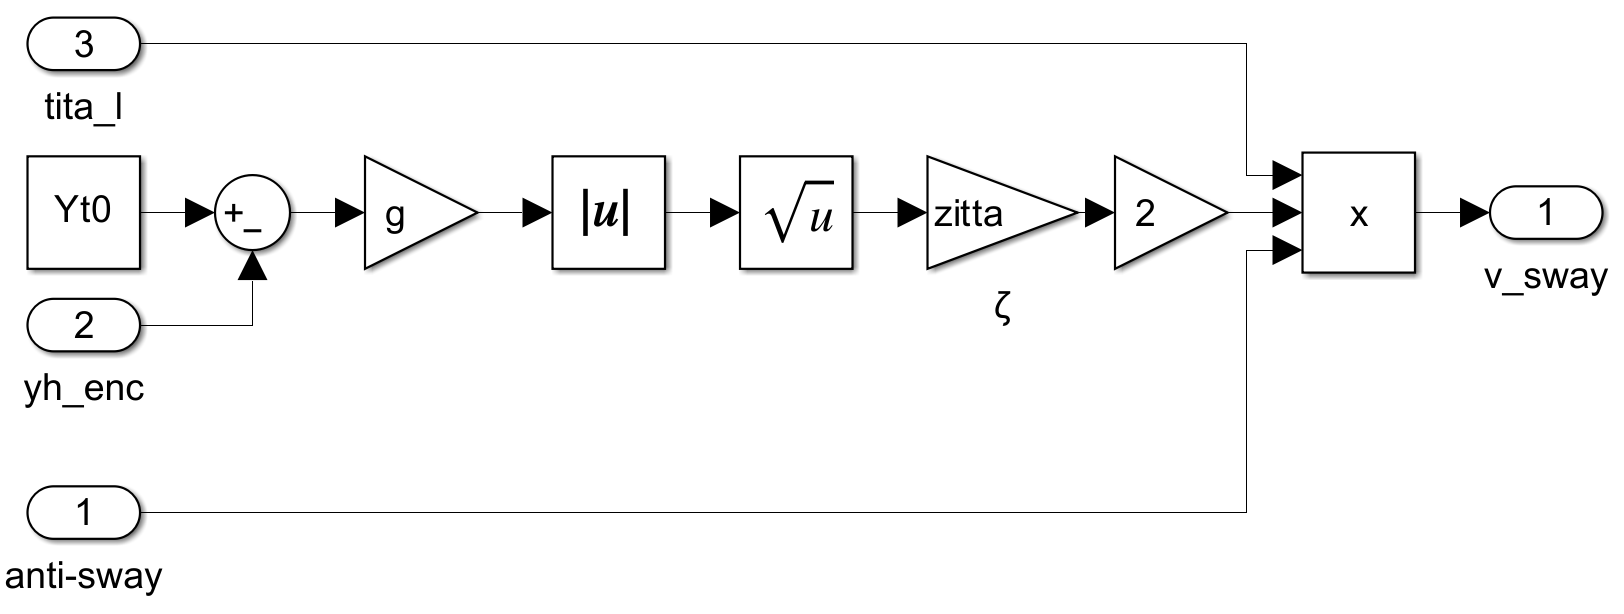
\includegraphics[width=0.8\linewidth]{nivel_2/control_balanceo.png}
      \end{column}
    \end{columns}
  \end{block}

  \begin{alertblock}{En la práctica}
    El amortiguamiento crítico ($\zeta=1$) sobrecorrige la posición; se usa $\zeta = 0.5$
    (subamortiguado) para mantener la carga cerca del objetivo.
  \end{alertblock}
\end{frame}

% \lautimode
\begin{frame}{Observador de estado del carro: motivación}
  \begin{block}{Problema de medición}
    \begin{itemize}
      \item Encoder mide solo \textbf{posición angular} $\theta_{tm}(t)$
      \item El controlador PI necesita \textbf{velocidad angular} $\omega_{tm}(t)$
      \item No se puede derivar la posición directamente (ruido, inestabilidad)
    \end{itemize}
  \end{block}

  \vspace{0.1cm}
  \begin{alertblock}{Solución}
    Implementar un \textbf{observador de estado} que estime $\tilde{\omega}_{tm}(t)$ a partir de la medición de $\theta_{tm}(t)$
  \end{alertblock}

  \vspace{0.2cm}
  \begin{block}{Complicación adicional}
    El observador convencional presenta \textbf{error en régimen permanente} ante perturbaciones constantes (balanceo de carga)
    \begin{itemize}
      \item Solución: agregar \textbf{acción integral} sobre el error de observación
    \end{itemize}
  \end{block}
\end{frame}

\begin{frame}{Modelo del carro en forma de estado}
  \begin{block}{Sistema simplificado (de la Ec. del accionamiento del carro)}
    \[
    \begin{cases}
      \dot{\theta}_{tm}(t) = \omega_{tm}(t) \\[6pt]
      \dot{\omega}_{tm}(t) = -\frac{b_{t,eq}}{J_{t,eq}}\omega_{tm}(t) + \frac{1}{J_{t,eq}}T_{tm}^*(t)
    \end{cases}
    \]
  \end{block}

  \vspace{-0.1cm}
  \begin{block}{Forma matricial: $\dot{\mathbf{x}} = A\mathbf{x} + B_c u$ ; $y = C\mathbf{x}$}
    \[
    \begin{bmatrix}
      \dot{\theta}_{tm}(t) \\
      \dot{\omega}_{tm}(t)
    \end{bmatrix}
    =
    \begin{bmatrix}
      0 & 1 \\
      0 & -\frac{b_{t,eq}}{J_{t,eq}}
    \end{bmatrix}
    \begin{bmatrix}
      \theta_{tm}(t) \\
      \omega_{tm}(t)
    \end{bmatrix}
    +
    \begin{bmatrix}
      0 \\
      \frac{1}{J_{t,eq}}
    \end{bmatrix}
    T_{tm}^*(t)
    \]
    \[
    y(t) = \begin{bmatrix} 1 & 0 \end{bmatrix}
    \begin{bmatrix}
      \theta_{tm}(t) \\
      \omega_{tm}(t)
    \end{bmatrix}
    = \theta_{tm}(t)
    \]
  \end{block}
\end{frame}

\begin{frame}{Problema: error del observador en régimen permanente}
  \begin{block}{Observador de Luenberger convencional}
    \[
    \dot{\hat{\mathbf{x}}} = (A - K_e C) \hat{\mathbf{x}} + B_c u + K_e y
    \]
    con matriz de ganancia $K_e = \begin{bmatrix} k_{\theta t} \\ k_{\omega t} \end{bmatrix}$
  \end{block}

  \vspace{-0.1cm}
  \begin{alertblock}{Limitación}
    Como el sistema es de \textbf{orden 2} y solo hay una salida medida, el observador no puede rechazar perturbaciones constantes desconocidas (como balanceo de carga)
    \begin{itemize}
      \item Resultado: error residual en la estimación de velocidad
    \end{itemize}
  \end{alertblock}

  \vspace{0.1cm}
  \begin{block}{Solución: sistema aumentado con integrador}
    Agregar un estado integrador $x_I(t)$ que acumule el error de observación:
    \[
    \dot{x}_I(t) = y(t) - \tilde{y}(t) = \theta_{tm}(t) - \tilde{\theta}_{tm}(t)
    \]
    La acción de este integrador se inyecta como control adicional en la dinámica estimada
  \end{block}
\end{frame}

\begin{frame}{Sistema aumentado del observador}
  \begin{block}{Estado ampliado}
    \[
    \tilde{\mathbf{x}}_{\text{aug}}(t) = \begin{bmatrix} \tilde{\theta}_{tm}(t) \\ \tilde{\omega}_{tm}(t) \\ x_I(t) \end{bmatrix}
    \]
  \end{block}

  \vspace{-0.15cm}
  \begin{block}{Ecuaciones del observador aumentado}
    \[
    \begin{bmatrix}
      \dot{\tilde{\theta}}_{tm}(t) \\
      \dot{\tilde{\omega}}_{tm}(t) \\
      \dot{x}_I(t)
    \end{bmatrix}
    =
    \begin{bmatrix}
      -k_{\theta t} & 1 & 0 \\
      -k_{\omega t} & -\frac{b_{t,eq}}{J_{t,eq}} & k_{it} \\
      -1 & 0 & 0
    \end{bmatrix}
    \begin{bmatrix}
      \tilde{\theta}_{tm}(t) \\
      \tilde{\omega}_{tm}(t) \\
      x_I(t)
    \end{bmatrix}
    +
    \begin{bmatrix}
      0 \\
      \frac{1}{J_{t,eq}} \\
      0
    \end{bmatrix}
    T_{tm}^*(t)
    +
    \begin{bmatrix}
      k_{\theta t} \\
      k_{\omega t} \\
      1
    \end{bmatrix}
    \theta_{tm}(t)
    \]
  \end{block}

  \vspace{-0.1cm}
  \begin{block}{Salida estimada}
    \[
    \tilde{y}(t) = \tilde{\theta}_{tm}(t)
    \]
  \end{block}
\end{frame}

\begin{frame}{Asignación de polos del observador}
  \begin{block}{Polinomio característico aumentado (3×3)}
    \[
    p(s) = \det(sI - A_{\text{aug}}) = s^3 + s^2 \left( k_{\theta t}+\frac{b_{t,eq}}{J_{t,eq}}\right) + s\left( k_{\omega t}+k_{\theta t}\frac{b_{t,eq}}{J_{t,eq}}\right) + k_{it}
    \]
  \end{block}

  \vspace{-0.15cm}
  \begin{block}{Especificación: polinomio deseado}
    Tres polos coincidentes en $\omega_{\text{obs}, t} = -\frac{b_{t,eq}}{J_{t,eq}}$ (el polo dominante):
    \[
    p_d(s) = (s + \omega_{\text{obs}, t})^3 = s^3 + 3\,\omega_{\text{obs}, t}\, s^2 + 3\,\omega_{\text{obs}, t}^2\, s + \omega_{\text{obs}, t}^3
    \]
  \end{block}

  \vspace{-0.15cm}
  \begin{block}{Igualación de coeficientes}
    \begin{align*}
      k_{\theta t} &= 3\, \omega_{\text{obs}, t}-\frac{b_{t,eq}}{J_{t,eq}} \\[4pt]
      k_{\omega t} &= 3\, \omega_{\text{obs}, t}^2 - k_{\theta t}\frac{b_{t,eq}}{J_{t,eq}} \\[4pt]
      k_{it} &= \omega_{\text{obs}, t}^3
    \end{align*}
  \end{block}
\end{frame}

\begin{frame}{Sintonía por separación de anchos de banda}
  \begin{block}{Principio de separación de dinámicas}
    Para garantizar que el observador no introduzca retardo de fase en el lazo regulatorio:
    \begin{itemize}
      \item Dinámica del observador $\gg$ dinámica de la planta a lazo abierto
      \item El observador debe ser \textbf{significativamente más rápido}
    \end{itemize}
  \end{block}

  \vspace{0.1cm}
  \begin{block}{Especificación}
    \[
    \omega_{\text{obs}, t} = 20 \times \left| -\frac{b_{t,eq}}{J_{t,eq}} \right|
    \]
    El observador es \textbf{20 veces más rápido} que el polo dominante de la planta
  \end{block}

  \vspace{0.15cm}
  \begin{alertblock}{Justificación}
    Esta separación asegura que:
    \begin{itemize}
      \item La estimación de velocidad es precisa con bajo retardo
      \item El controlador PI vea un sistema prácticamente ideal (sin dinámica del observador)
      \item No hay degradación de estabilidad por la estimación
    \end{itemize}
  \end{alertblock}
\end{frame}

\begin{frame}{Ecuaciones implementadas en Simulink}
  \begin{block}{Las tres ecuaciones diferenciales a integrar}
    \[
    \begin{cases}
      \dot{\tilde{\theta}}_{tm}(t) = \tilde{\omega}_{tm}(t) + k_{\theta t}\left(\theta_{tm}(t)-\tilde{\theta}_{tm}(t)\right) \\[6pt]
      \dot{\tilde{\omega}}_{tm}(t) = \frac{1}{J_{t,eq}}T_{tm}^*(t) + k_{\omega t}\left(\theta_{tm}(t)-\tilde{\theta}_{tm}(t)\right) + k_{it}\,x_I(t) \\[6pt]
      \dot{x}_I(t) = \theta_{tm}(t)-\tilde{\theta}_{tm}(t)
    \end{cases}
    \]
  \end{block}

  \vspace{0.1cm}
  \begin{block}{Salidas del observador}
    \begin{itemize}
      \item Velocidad estimada: $\tilde{\omega}_{tm}(t)$ $\Rightarrow$ al controlador PI
      \item Posición estimada: $\tilde{\theta}_{tm}(t)$ $\Rightarrow$ validación
    \end{itemize}
  \end{block}

  \begin{alertblock}{Entrada}
    \begin{itemize}
      \item Medición del encoder: $\theta_{tm}(t)$
      \item Comando de torque: $T_{tm}^*(t)$ (ya disponible del PI)
    \end{itemize}
  \end{alertblock}
\end{frame}

\begin{frame}{Diagrama de bloques: Observador + PI del carro}
  \centering
  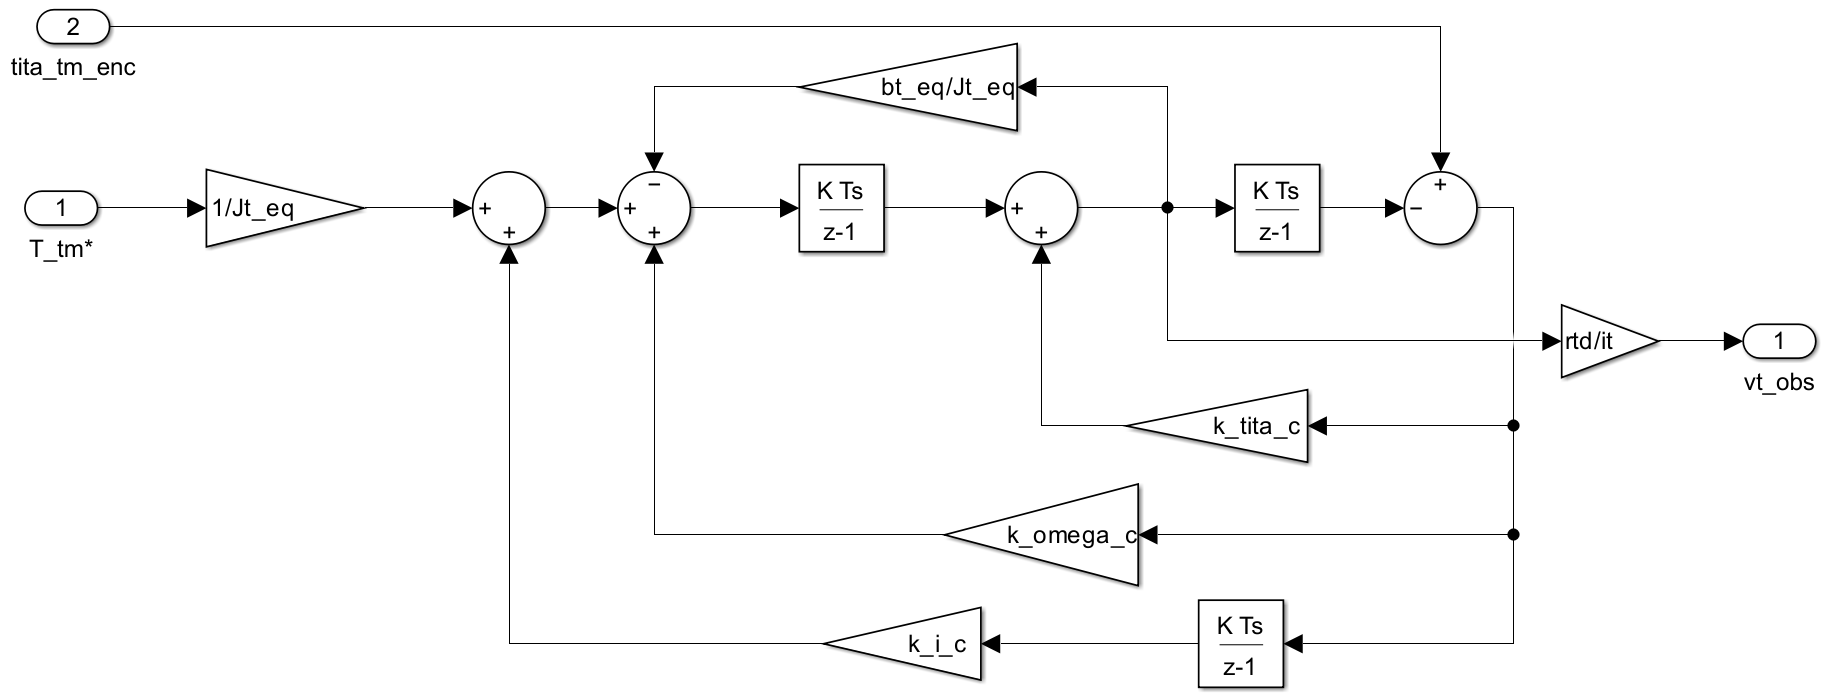
\includegraphics[width=0.9\textwidth]{nivel_2/obs_pid_carro.png}
  
  \vspace{0.2cm}
  \begin{block}{Flujo de señales}
    \begin{itemize}
      \item Encoder → Observador (estima $\tilde{\omega}_{tm}$)
      \item $v_t^*$, $\tilde{\omega}_{tm}$ → PI (calcula $T_{tm}^*$)
      \item $T_{tm}^*$ → Modulador de torque → Planta
    \end{itemize}
  \end{block}
\end{frame}

% \defaultmode
\begin{frame}{Modelo de izaje para control de velocidad}
  \begin{block}{Balance de torques en el eje del motor}
    Agrupando las dinámicas externas en un torque de perturbación $T_{pert}$:
    \[
    J_{h,eq}\,\frac{d\omega_{hm}}{dt} + b_{h,eq}\,\omega_{hm} = T_{hm} - T_{pert}
    \]
    \[
    T_{pert} = \frac{F_{hw}\,r_{hd}}{i_h}
    \]
  \end{block}

  \vspace{-0.1cm}
  \begin{block}{Función de transferencia de la planta}
    \[
    G_{vel}(s) = \frac{\Omega_{hm}(s)}{T_{hm}(s)} = \frac{1}{J_{h,eq}\,s + b_{h,eq}}
    \]
  \end{block}

  \begin{alertblock}{Casi un integrador}
    Fricción muy baja $\Rightarrow$ polo $P_{mec}=-b_{h,eq}/J_{h,eq}\approx 0$: la planta se
    comporta casi como un \textbf{integrador puro}.
  \end{alertblock}
\end{frame}

\begin{frame}{Diseño del lazo regulador (PI)}
  \begin{block}{Controlador y lazo cerrado}
    $C_{vel}(s) = K_p + \dfrac{K_i}{s}$, que da:
    \[
    T(s) = \frac{K_p\,s + K_i}{J_{h,eq}\,s^2 + (b_{h,eq}+K_p)\,s + K_i}
    \]
  \end{block}

  \vspace{-0.1cm}
  \begin{block}{Asignación de polos ($s^2+2\zeta\omega_n s+\omega_n^2$)}
    \[
    K_p = 2\,\zeta\,\omega_n\,J_{h,eq} + b_{h,eq} \quad ; \quad K_i = \omega_n^2\,J_{h,eq}
    \]
    Con $\omega_n \approx 8$ rad/s (rápido sin excitar la resonancia del cable) y $\zeta = 1$
    (sin sobrepaso).
  \end{block}

  \begin{alertblock}{Rigidez}
    Esta sintonía da la ``rigidez'' necesaria para \textbf{sostener la carga} suspendida.
  \end{alertblock}
\end{frame}

\begin{frame}{Compensación de gravedad (feedforward)}
  \begin{columns}[T]
    \begin{column}{0.6\textwidth}
      \begin{block}{Pre-alimentación del peso estático}
        \[
        T_{g,ff} = \frac{m_l(\sig{TLK})\,g\,r_{hd}}{2\,i_h}
        \]
        Ley de control del lazo: $\;T_{hm}^*(k) = T_{PI}(k) + T_{g,ff}$
      \end{block}
    \end{column}
    \begin{column}{0.4\textwidth}
      \begin{alertblock}{Ventaja}
        El término integral sólo corrige \textbf{errores de modelo}; el peso lo sostiene el
        feedforward $\Rightarrow$ respuesta más rápida y sin caída al arrancar.
      \end{alertblock}
    \end{column}
  \end{columns}

  \vspace{0.3cm}
  \centering
  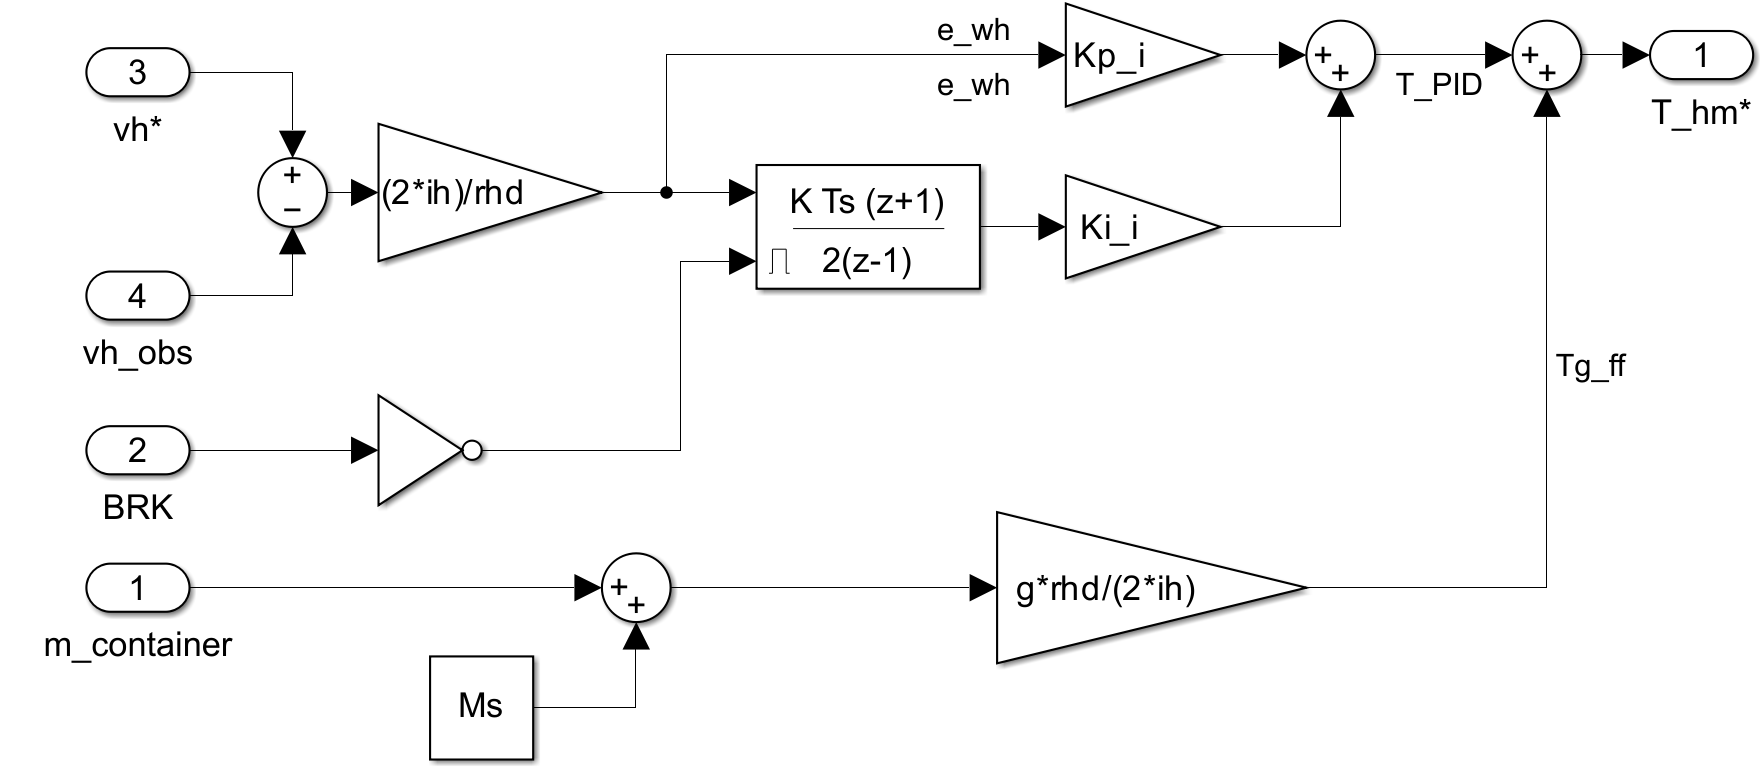
\includegraphics[width=0.72\linewidth]{nivel_2/lazo_controlador_izaje.png}
\end{frame}

\begin{frame}{Anti-windup y observador del izaje}
  \begin{columns}[T]
    \begin{column}{0.5\textwidth}
      \begin{block}{Anti-windup (dos frenos)}
        El izaje tiene freno de operación \sig{$BRK_h$} y de emergencia \sig{$BRK_{hE}$}:
        \textbf{cualquiera} de los dos resetea el integrador (igual criterio que el carro).
      \end{block}
    \end{column}
    \begin{column}{0.5\textwidth}
      \begin{block}{Observador con acción integral}
        Análogo al del carro, con las matrices del izaje. Ganancias por \textbf{separación de
        anchos de banda}: $\omega_{obs\,h} = 20\times$ el polo dominante de la planta, siendo $\omega_{obs\,h} = -9.5197\, rad/s$
      \end{block}
    \end{column}
  \end{columns}

  \vspace{0.3cm}
  \centering
  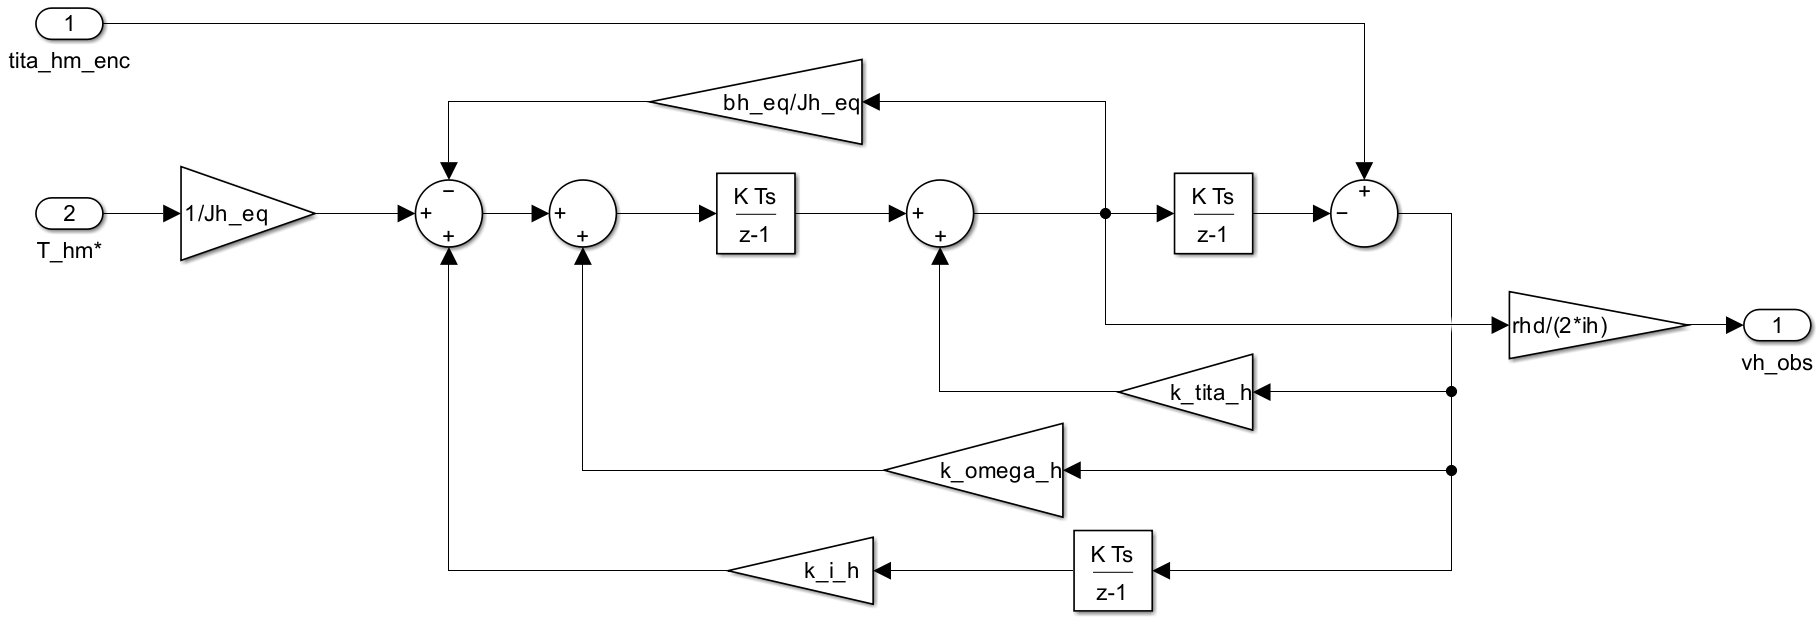
\includegraphics[width=0.78\linewidth]{nivel_2/obs_pid_izaje.png}
\end{frame}

\begin{frame}{Controlador regulatorio del carro (Simulink)}
  \centering
  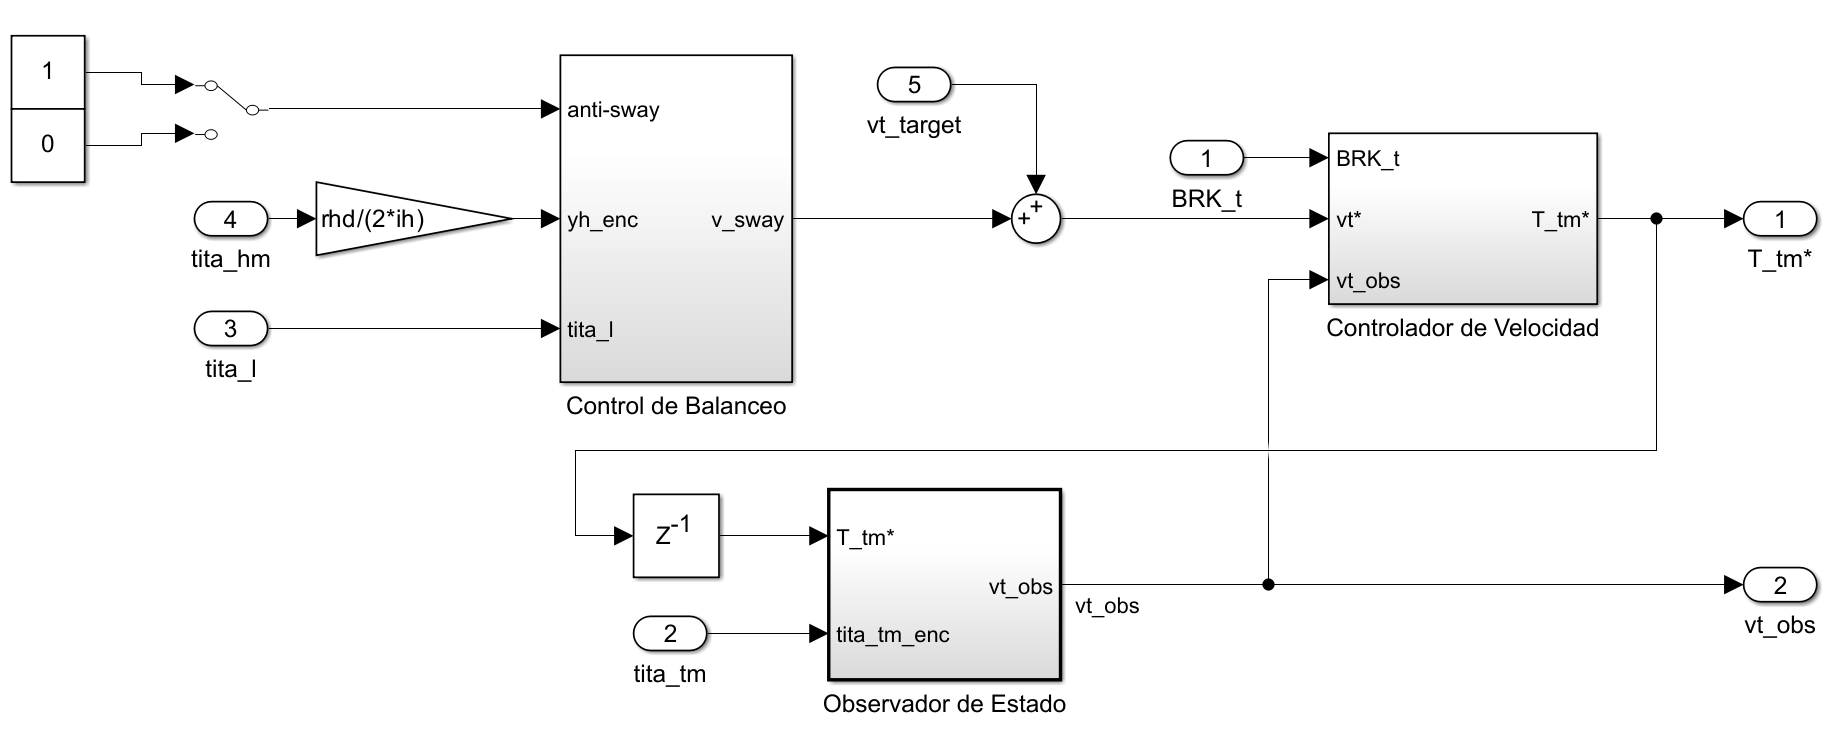
\includegraphics[width=\linewidth,height=0.82\textheight,keepaspectratio]{nivel_2/controlador_carro.png}
\end{frame}

\begin{frame}{Controlador regulatorio del izaje (Simulink)}
  \centering
  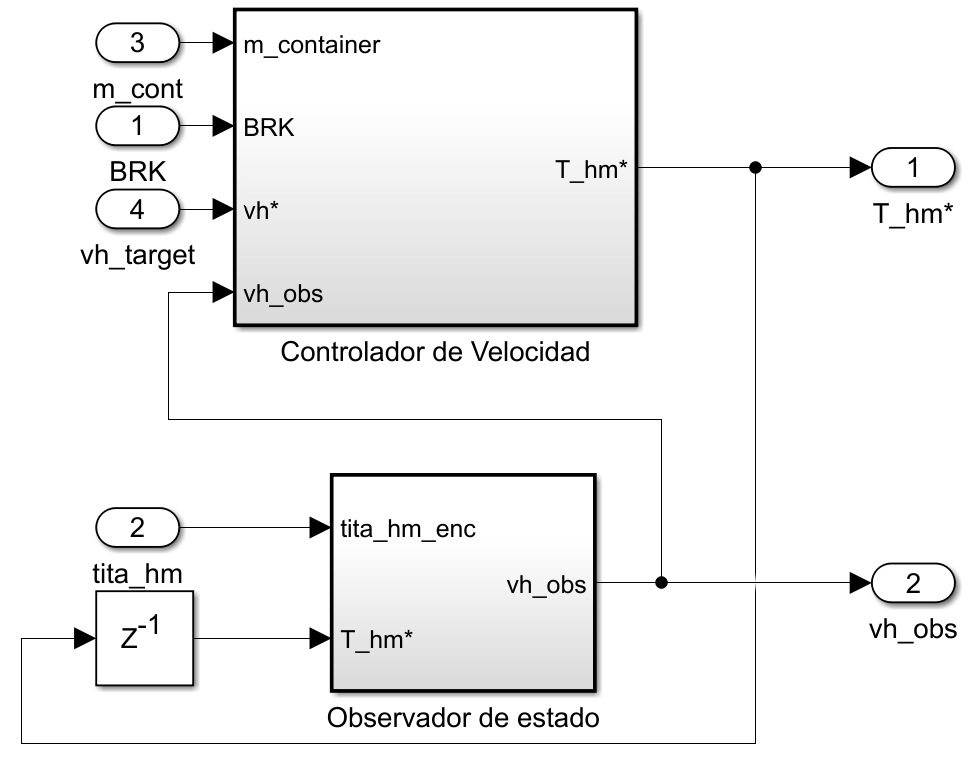
\includegraphics[width=\linewidth,height=0.82\textheight,keepaspectratio]{nivel_2/controlador_izaje.png}
\end{frame}

\section{Nivel 1 --- Control supervisor (DEDS)}

\begin{frame}{Nivel 1: el cerebro lógico de la grúa}
  Autómata de \textbf{eventos discretos} (Stateflow), $T_{s1}=20$ ms. Organizado en
  \textbf{procesos paralelos} que se evalúan simultáneamente:
  \begin{columns}[T]
    \begin{column}{0.5\textwidth}
      \begin{itemize}
        \item \textbf{Autómata principal} de modos.
        \item Gestión de \textbf{twistlocks}.
        \item Análisis espacial: \textbf{perfil e índices} (LIDAR).
      \end{itemize}
    \end{column}
    \begin{column}{0.5\textwidth}
      \begin{itemize}
        \item \textbf{Suavizado} de consignas (jerk/acel.).
        \item \textbf{Límites suaves} de velocidad.
        \item \textbf{Watchdog} de comunicación.
      \end{itemize}
    \end{column}
  \end{columns}
  \vspace{0.2cm}
  \begin{alertblock}{Entradas / Salidas}
    Sensores + joystick + fallas $\;\to\;$ consignas \sig{vx\_cmd}/\sig{vy\_cmd}, frenos
    \sig{$BRK$}, \sig{TLK}, \sig{vh\_lim}, \sig{heartbeat}.
  \end{alertblock}
\end{frame}

\begin{frame}{Autómata principal de modos de operación}
  \begin{columns}[T]
    \begin{column}{0.42\textwidth}
      \begin{itemize}
        \item \textbf{Reposo}: detenido, frenos cerrados.
        \item \textbf{Manual}: control directo por joystick.
        \item \textbf{Automático}: ciclo autónomo de carga/descarga.
        \item \textbf{Recuperación}: resguardo tras falla.
        \item \textbf{Errores}: por tipo de fin de carrera.
      \end{itemize}
    \end{column}
    \begin{column}{0.58\textwidth}
      \centering
      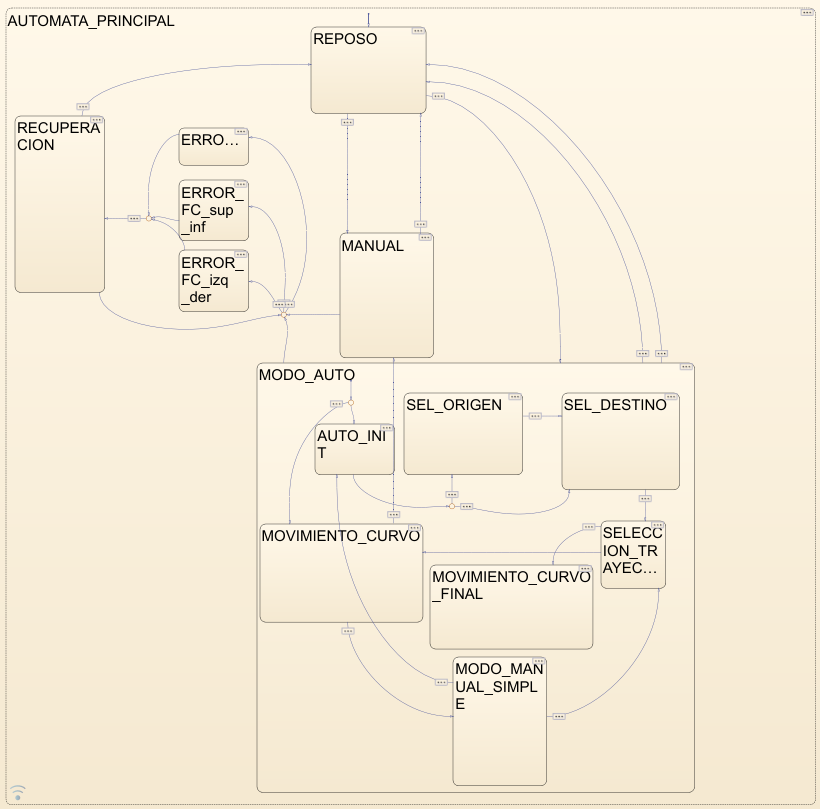
\includegraphics[width=\linewidth]{nivel_1/automata_principal.png}
    \end{column}
  \end{columns}
\end{frame}

\begin{frame}{Modo automático: ciclo coordinado sin colisiones}
  \begin{itemize}
    \item Secuencia \textbf{origen $\to$ destino} gestionada por el estado del ciclo y los
          índices seleccionados.
    \item Una \textbf{función planificadora} genera las consignas de velocidad
          (\sig{vx\_target}, \sig{vy\_target}) coordinando ambos ejes.
    \item Usa la \textbf{envolvente de seguridad} del perfil para \textbf{evadir colisiones}
          con la pila de contenedores.
    \item Movimientos \textbf{simultáneos} (izaje + traslación) para optimizar el tiempo de
          ciclo.
    \item \textbf{Transferencia suave} a manual si el operador interviene (\textit{bumpless}).
  \end{itemize}
\end{frame}

\begin{frame}{Gestión de twistlocks y estimación de carga}
  \begin{columns}[T]
    \begin{column}{0.5\textwidth}
      Cuatro estados: \texttt{VACIO} $\to$ \texttt{CERRANDO} $\to$ \texttt{CARGADO} $\to$
      \texttt{ABRIENDO}.
      \begin{itemize}
        \item Toma/libera la carga sólo con el spreader \textbf{apoyado} (interlock).
        \item \textbf{Estima la masa} del contenedor con la celda de carga.
        \item Detecta \textbf{sobrecarga} y limita la velocidad por curva de potencia
              (\sig{vh\_lim}).
      \end{itemize}
    \end{column}
    \begin{column}{0.5\textwidth}
      \centering
      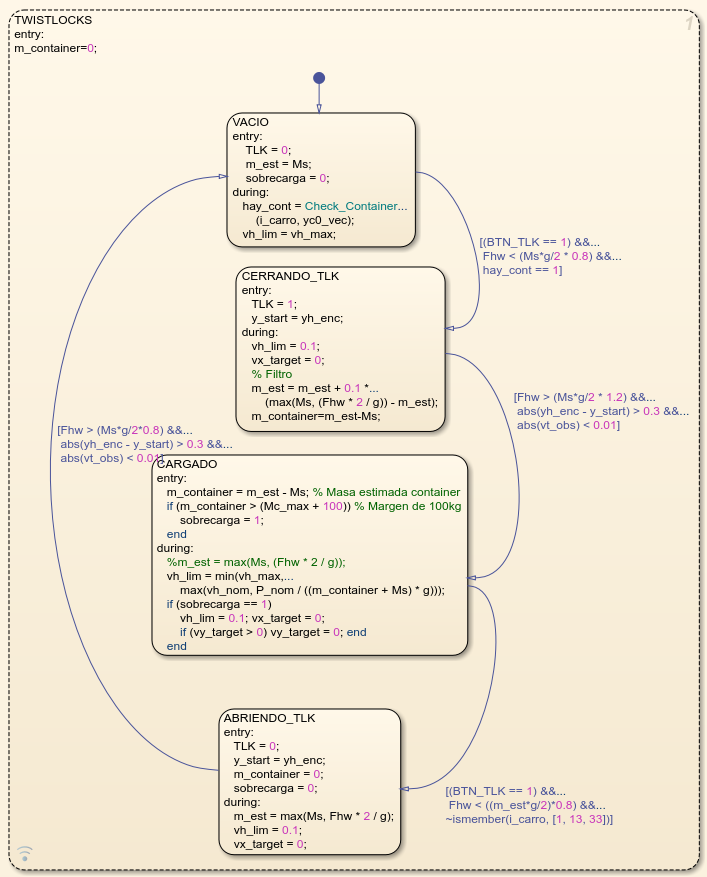
\includegraphics[width=\linewidth]{nivel_1/twistlocks.png}
    \end{column}
  \end{columns}
\end{frame}

\begin{frame}{Análisis espacial: perfil de obstáculos e índices}
  \begin{columns}[T]
    \begin{column}{0.5\textwidth}
      \begin{itemize}
        \item El \textbf{LIDAR} releva el perfil de alturas bajo el área de trabajo.
        \item Calcula los \textbf{índices discretos} del carro y la cruceta.
        \item Genera una \textbf{envolvente de seguridad} (márgenes laterales/superiores).
        \item Habilitación del modo automático: perfil \textbf{escaneado por completo}.
      \end{itemize}
    \end{column}
    \begin{column}{0.5\textwidth}
      \centering
      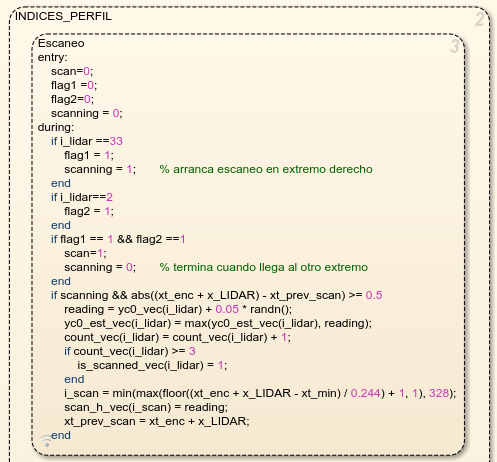
\includegraphics[width=\linewidth]{nivel_1/indices_perfil.png}
    \end{column}
  \end{columns}
\end{frame}

\begin{frame}{Suavizado y límites suaves de velocidad}
  \begin{columns}[T]
    \begin{column}{0.5\textwidth}
      \begin{block}{Suavizado (jerk/aceleración)}
        Convierte consignas crudas en \sig{vx\_suave}/\sig{vy\_suave} graduales; clave en modo
        manual.
      \end{block}
      \centering
      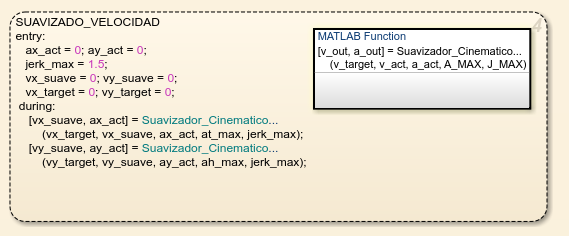
\includegraphics[width=0.85\linewidth]{nivel_1/suavizado_velocidad.png}
    \end{column}
    \begin{column}{0.5\textwidth}
      \begin{block}{Límites suaves (frenado anticipado)}
        $v_{segura}=\sqrt{2\,a\,d}$ con retardo dinámico: recorta la velocidad cerca de los
        límites, antes de los fines de carrera.
      \end{block}
      \centering
      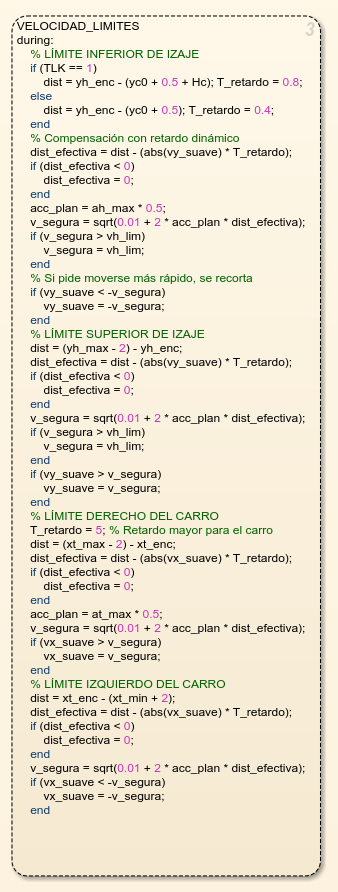
\includegraphics[width=0.42\linewidth]{nivel_1/limites_suaves.png}
    \end{column}
  \end{columns}
\end{frame}

\begin{frame}{Watchdog y manejo del joystick}
  \begin{columns}[T]
    \begin{column}{0.5\textwidth}
      \textbf{Watchdog (heartbeat)}
      \begin{itemize}
        \item Emite un latido periódico al Nivel 0.
        \item Su ausencia $\Rightarrow$ pérdida de comunicación $\Rightarrow$ parada de
              emergencia.
      \end{itemize}
      \centering
      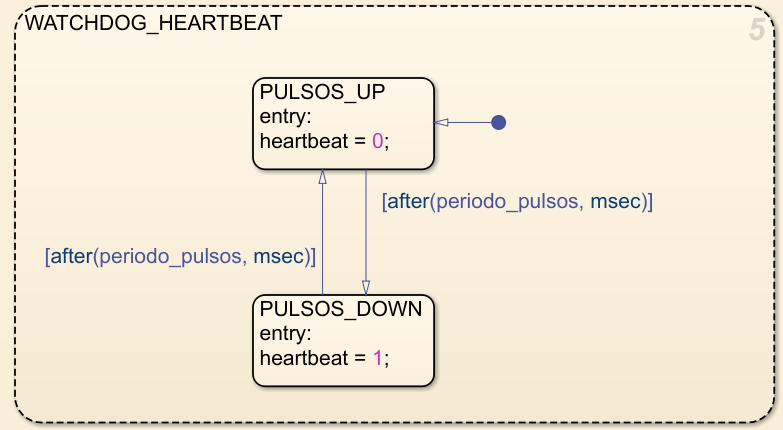
\includegraphics[width=0.7\linewidth]{nivel_1/watchdog_heartbeat.png}
    \end{column}
    \begin{column}{0.5\textwidth}
      \textbf{Joystick y botones}
      \begin{itemize}
        \item Ejes $\to$ velocidad de carro e izaje.
        \item Botones $\to$ TLK, modo manual/auto, reset, emergencia.
      \end{itemize}
      \centering
      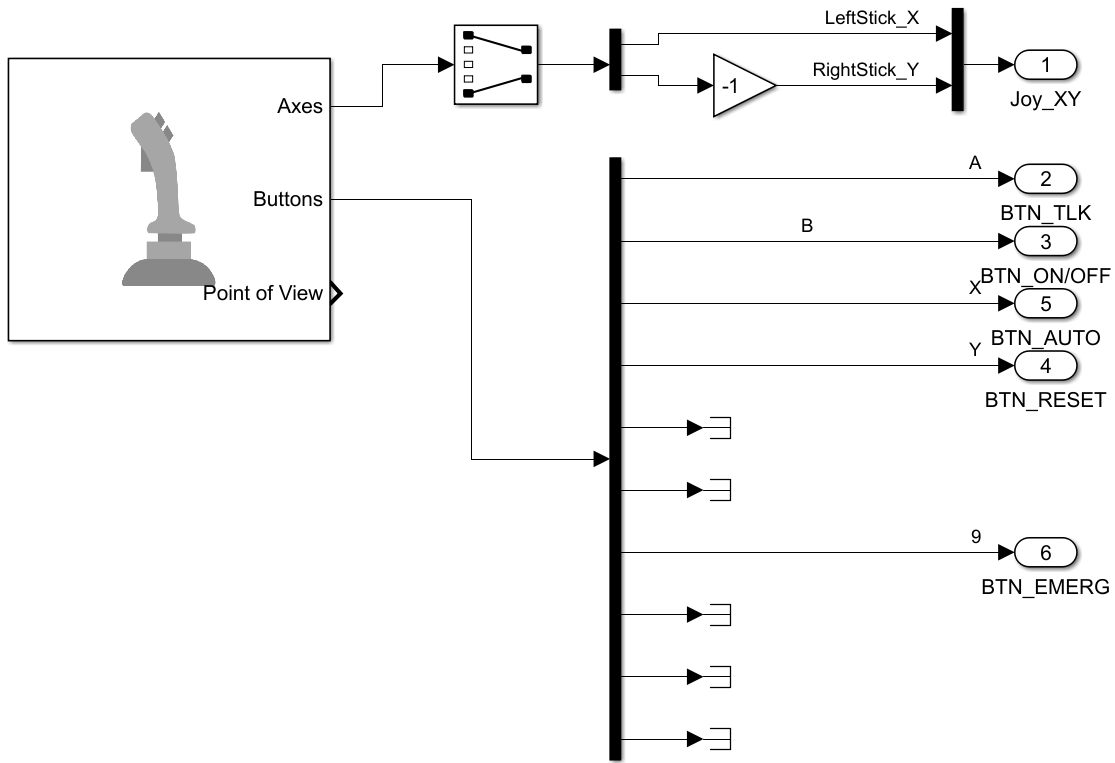
\includegraphics[width=\linewidth]{nivel_1/joystick.png}
    \end{column}
  \end{columns}
\end{frame}

% \lautimode
\section{Nivel 1 --- Control supervisor (DEDS)}

\begin{frame}{Twistlocks}
  \begin{columns}[T]
    \begin{column}{0.5\textwidth}
      Cuatro estados: \texttt{VACIO} $\to$ \texttt{CERRANDO} $\to$ \texttt{CARGADO} $\to$
      \texttt{ABRIENDO}.
      \begin{itemize}
        \item Toma/libera la carga sólo con el spreader \textbf{apoyado} (interlock).
        \item \textbf{Estima la masa} del contenedor con la celda de carga.
        \item Detecta \textbf{sobrecarga} y limita la velocidad por curva de potencia.
          \begin{equation*}
        v_{h,lim}({m}_l) = 
        \begin{cases} 
            v_{h\max} & \text{si } {m}_l < 32500 kg \\
            \frac{P_{h\ nom}}{{m}_l \, g} & \text{si } {m}_l \ge 32500 kg
        \end{cases}
    \end{equation*}
      \end{itemize}
    \end{column}
    \begin{column}{0.5\textwidth}
      \centering
      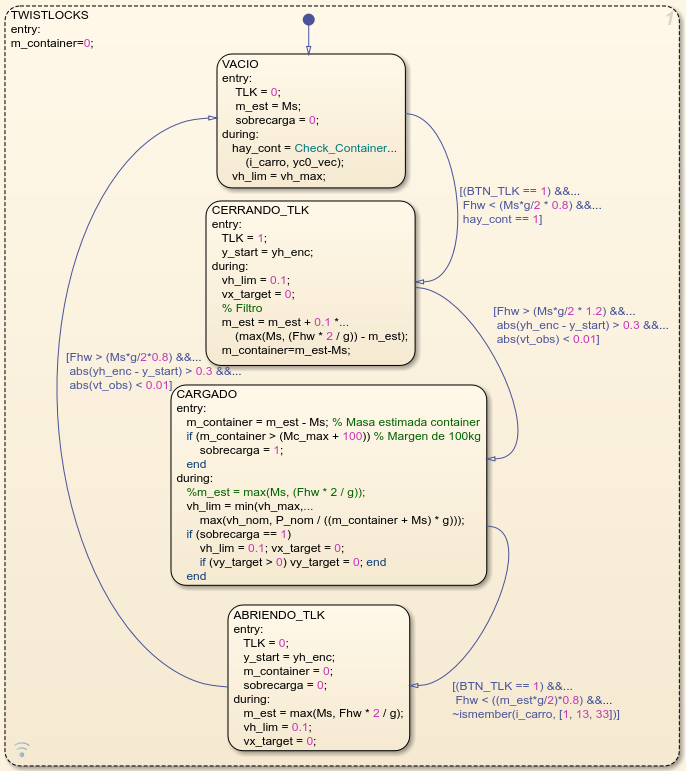
\includegraphics[height=0.95\textheight]{nivel_1/twistlocks_p.png}
    \end{column}
  \end{columns}
\end{frame}

\begin{frame}{Análisis espacial}
      \centering
      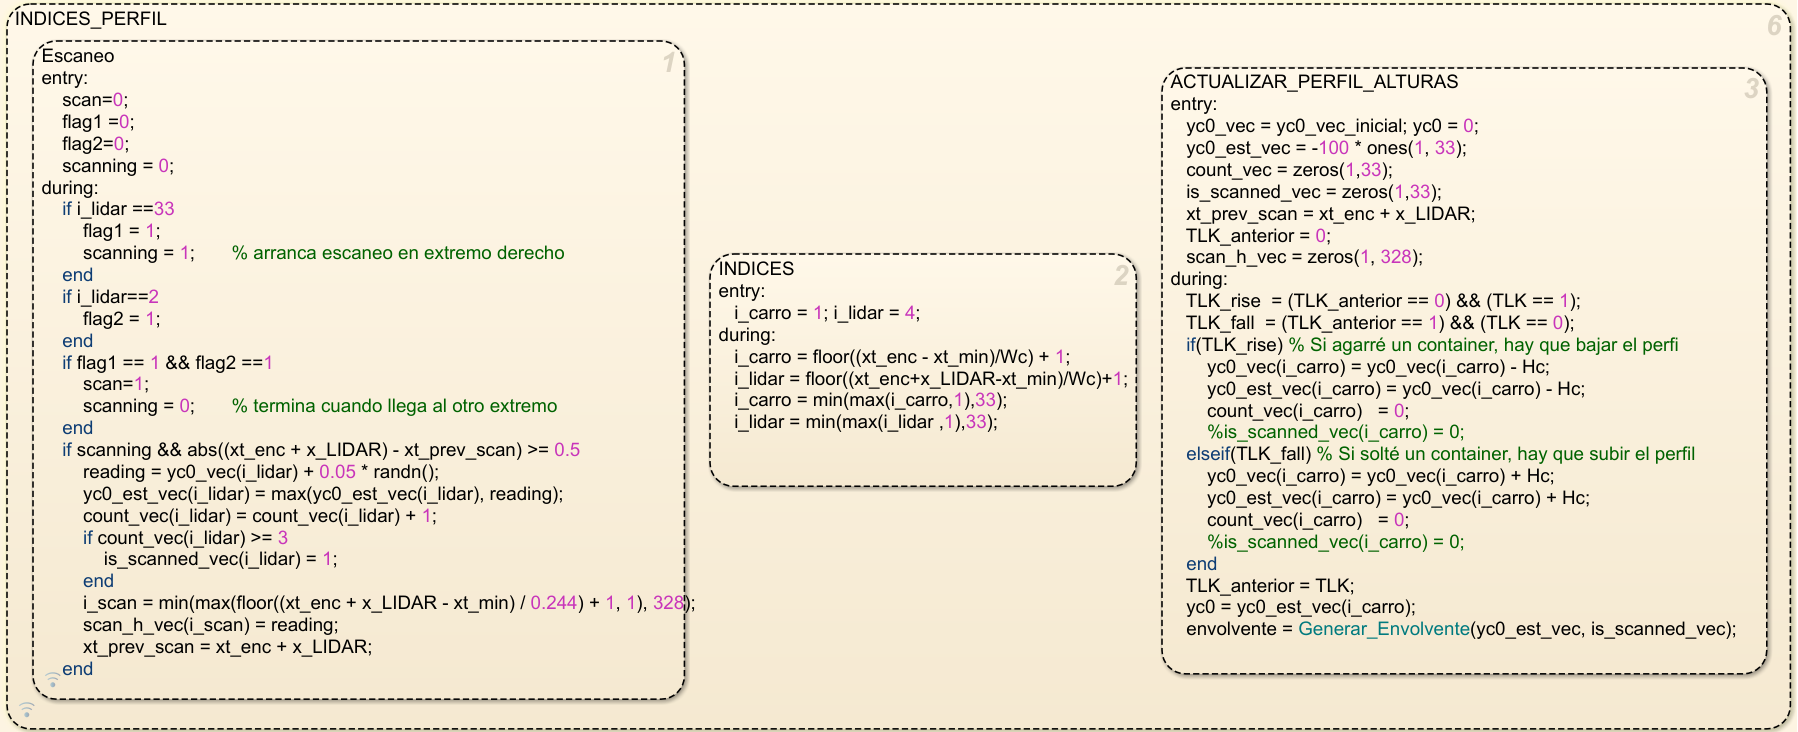
\includegraphics[width=\linewidth]{nivel_1/indices_perfil_p.png}
\end{frame}

\begin{frame}{Límites suaves de velocidad}
      \begin{columns}[T]
        \begin{column}{0.48\textwidth}
          \centering
          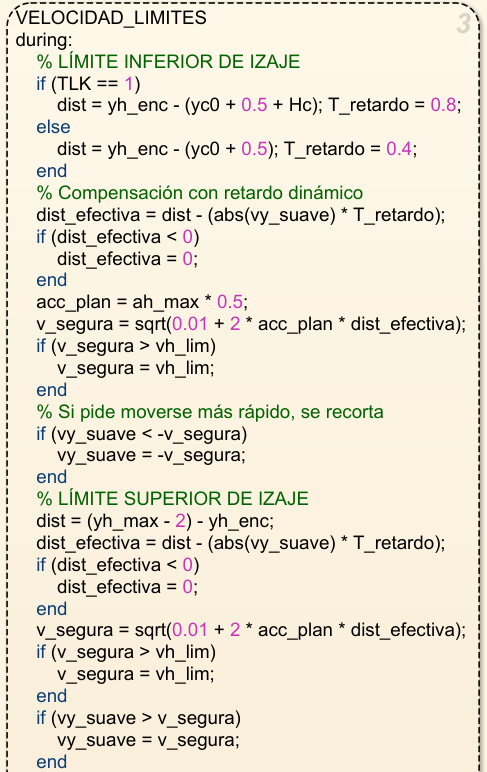
\includegraphics[width=0.7\textwidth]{nivel_1/limites1.png}
        \end{column}
        \begin{column}{0.48\textwidth}
          \centering
          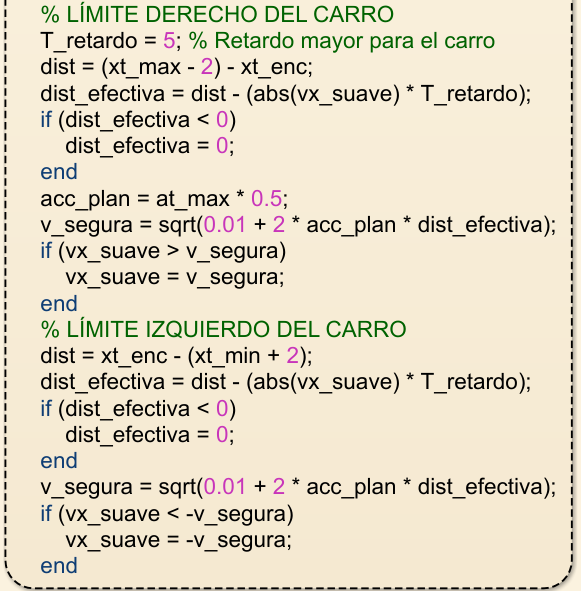
\includegraphics[width=\textwidth]{nivel_1/limites2.png}
        \end{column}
      \end{columns}
\end{frame}

\begin{frame}{Suavizado y watchdog}
  \begin{columns}[T]
     \begin{column}{0.5\textwidth}
      \begin{block}{Suavizado}
        Convierte consignas crudas en $v_{suave}$.
      \end{block}
      \centering
      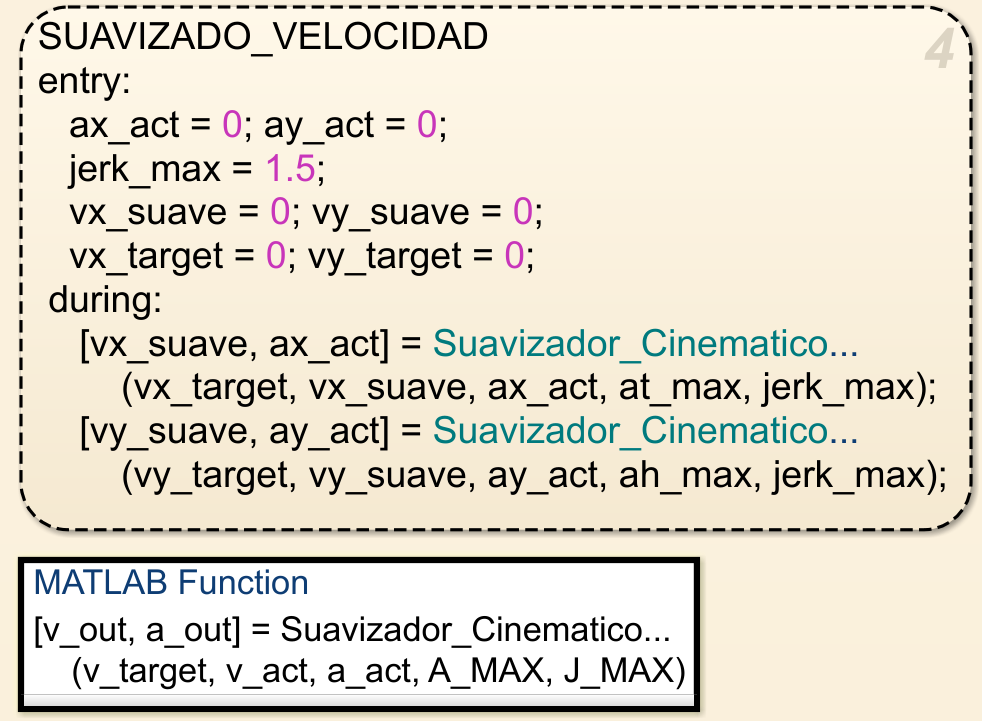
\includegraphics[width=\linewidth]{nivel_1/suavizado_p.png}
    \end{column}
    \begin{column}{0.5\textwidth}
      \begin{block}{Watchdog}
        Genera un heartbeat cada cierto tiempo que recibe el Nivel 0.
      \end{block}
      \centering
      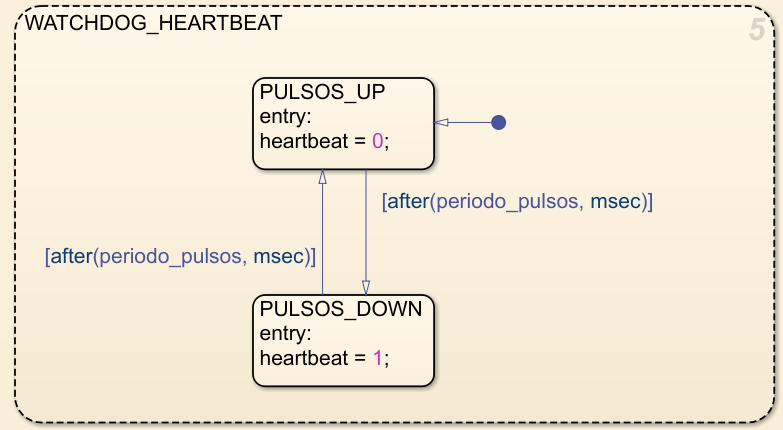
\includegraphics[width=\linewidth]{nivel_1/watchdog_heartbeat.png}
    \end{column}
  \end{columns}
\end{frame}

% \defaultmode
% \lautimode
\section{Nivel 0 --- Protección}

\begin{frame}{Nivel 0}
  \begin{itemize}
    \item Capa de protección más baja, pero con mayor jerarquía.
    \item Salvaguarda la integridad de la grúa, la carga y el personal.
    \item Autoridad para sobrescribir cualquier comando del Nivel 1, cortando energía y aplicando frenos.
    \item Supervisa la planta de forma \textbf{permanente} (redundancia de sensores).
  \end{itemize}
\end{frame}

\begin{frame}{Autómata de seguridad: frenado selectivo}
  \begin{columns}[T]
    \begin{column}{0.45\textwidth}
      \begin{itemize}
        \item Estado nominal \texttt{SISTEMA\_OK} (ambos frenos abiertos).
        \item \textbf{Frenado selectivo}: sólo se detiene el \textbf{eje afectado}.
          \begin{itemize}
            \item Falla izaje $\Rightarrow$ frena izaje, carro libre.
            \item Falla carro $\Rightarrow$ frena carro, izaje libre.
            \item Emergencia manual $\Rightarrow$ ambos.
          \end{itemize}
        \item Rearme manual $\to$ \texttt{RECUPERACION}.
      \end{itemize}
    \end{column}
    \begin{column}{0.55\textwidth}
      \centering
      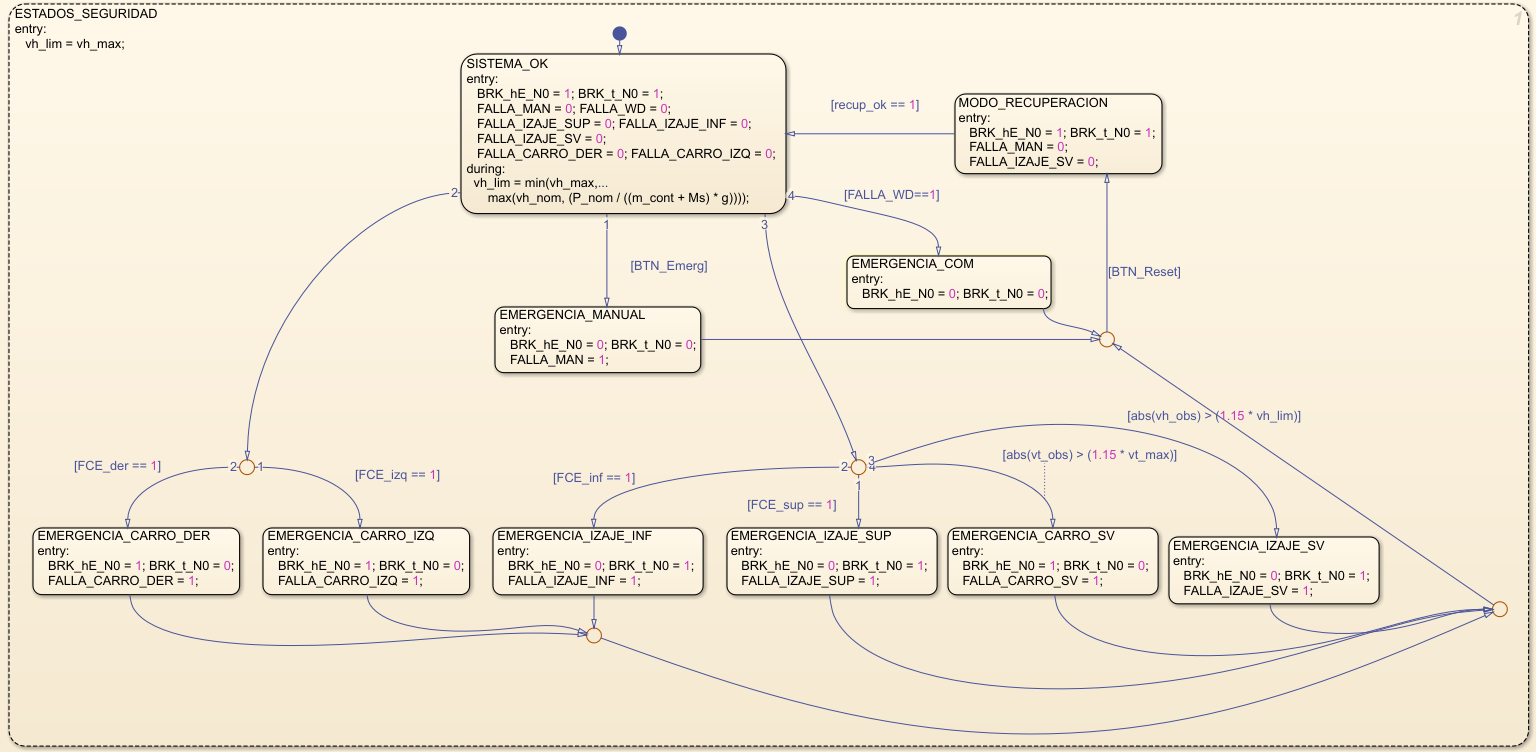
\includegraphics[width=\linewidth]{nivel_0/estados_seguridad.png}
    \end{column}
  \end{columns}
\end{frame}

\begin{frame}{Monitor de comunicaciones}
  \begin{columns}[T]
    \begin{column}{0.4\textwidth}
      \begin{itemize}
        \item Persigue el \textbf{heartbeat} del supervisor.
        \item Si el contador supera el límite seguro $FALLA_{WD}$.
        \item Dispara la parada de emergencia.
      \end{itemize}
    \end{column}
    \begin{column}{0.6\textwidth}
      \centering
      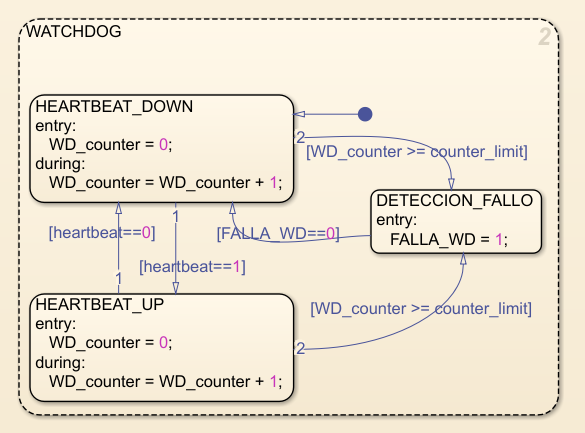
\includegraphics[width=\linewidth]{nivel_0/watchdog.png}
    \end{column}
  \end{columns}
\end{frame}



\section{Comunicación y Animación con Python}

\begin{frame}{Integración completa en Simulink}
  \centering
  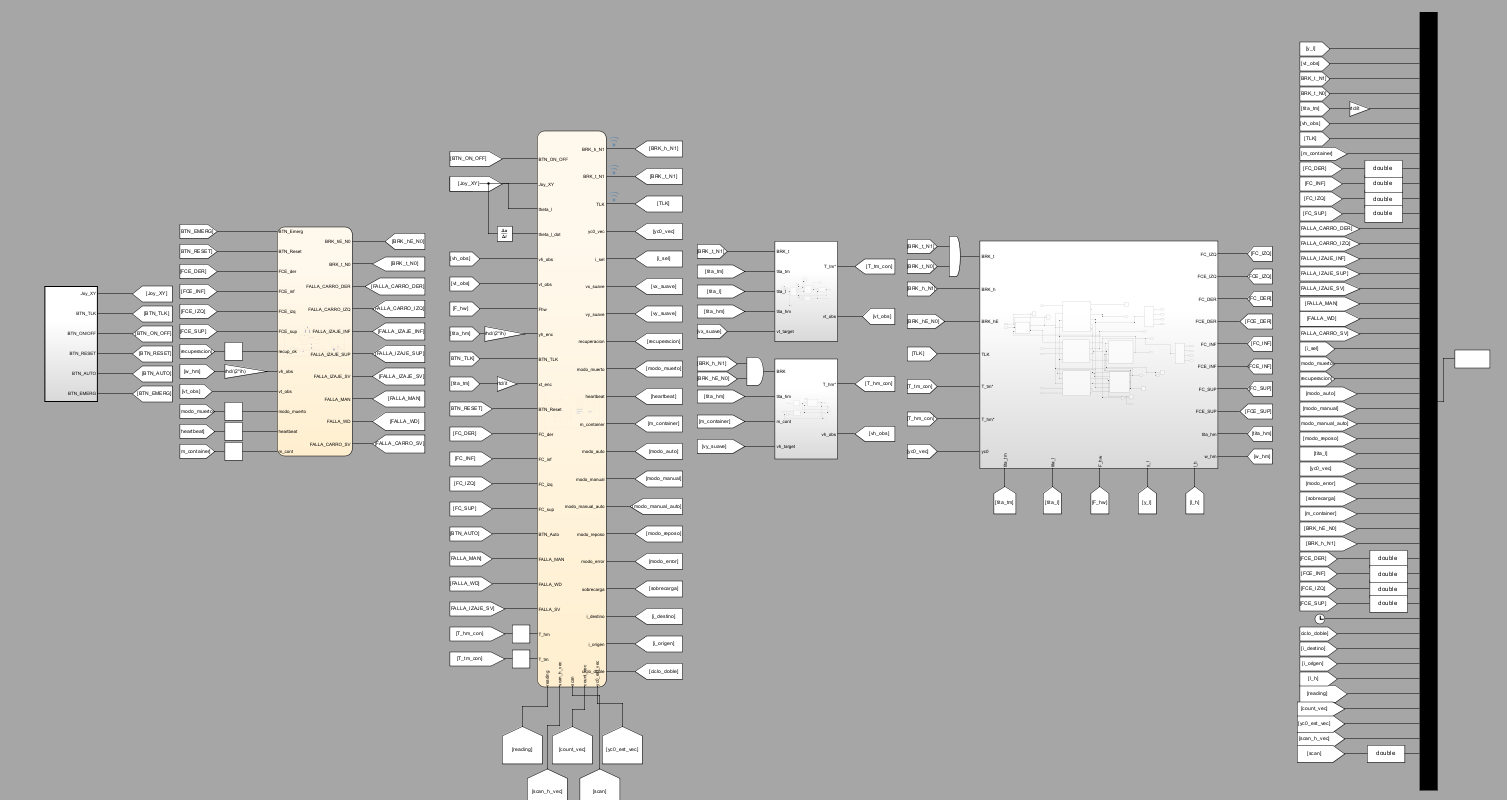
\includegraphics[width=0.95\textwidth]{simulacion/planta_completa.png}
  
  \vspace{0.2cm}
  Planta física + Nivel 2 (control) + Nivel 1 (supervisor) + Nivel 0 (protección) + UDP
\end{frame}

\begin{frame}{Comunicación UDP: Simulink Python}
  \centering
  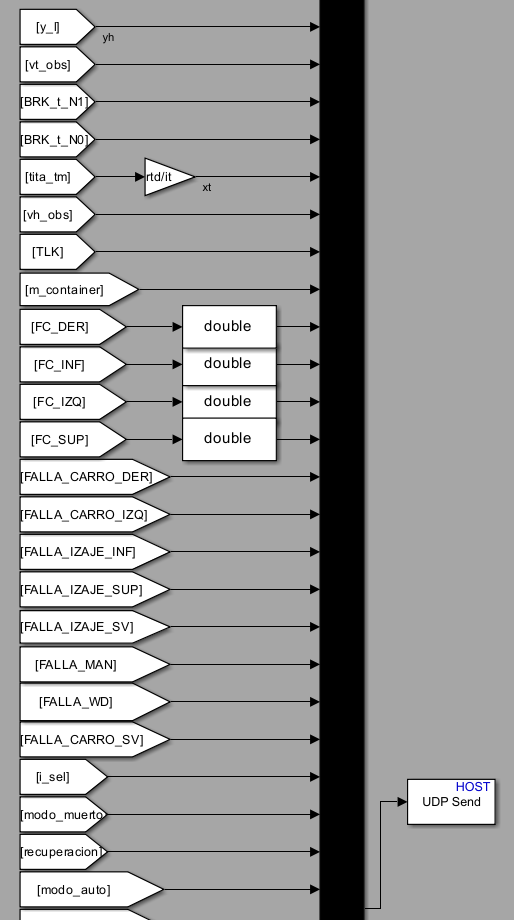
\includegraphics[width=0.32\textwidth]{simulacion/sim_udp.png}
  \hspace{0.3cm}
  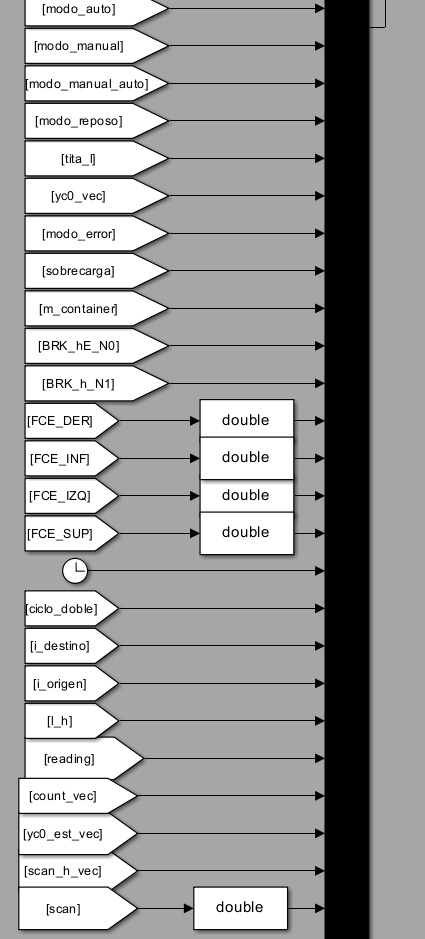
\includegraphics[width=0.32\textwidth]{simulacion/sim_udp2.png}
  
  \vspace{0.2cm}
  Estados de la planta (posiciones, velocidades, sensores) Visualización web en tiempo real
\end{frame}

\begin{frame}{Modo manual}
  \centering
  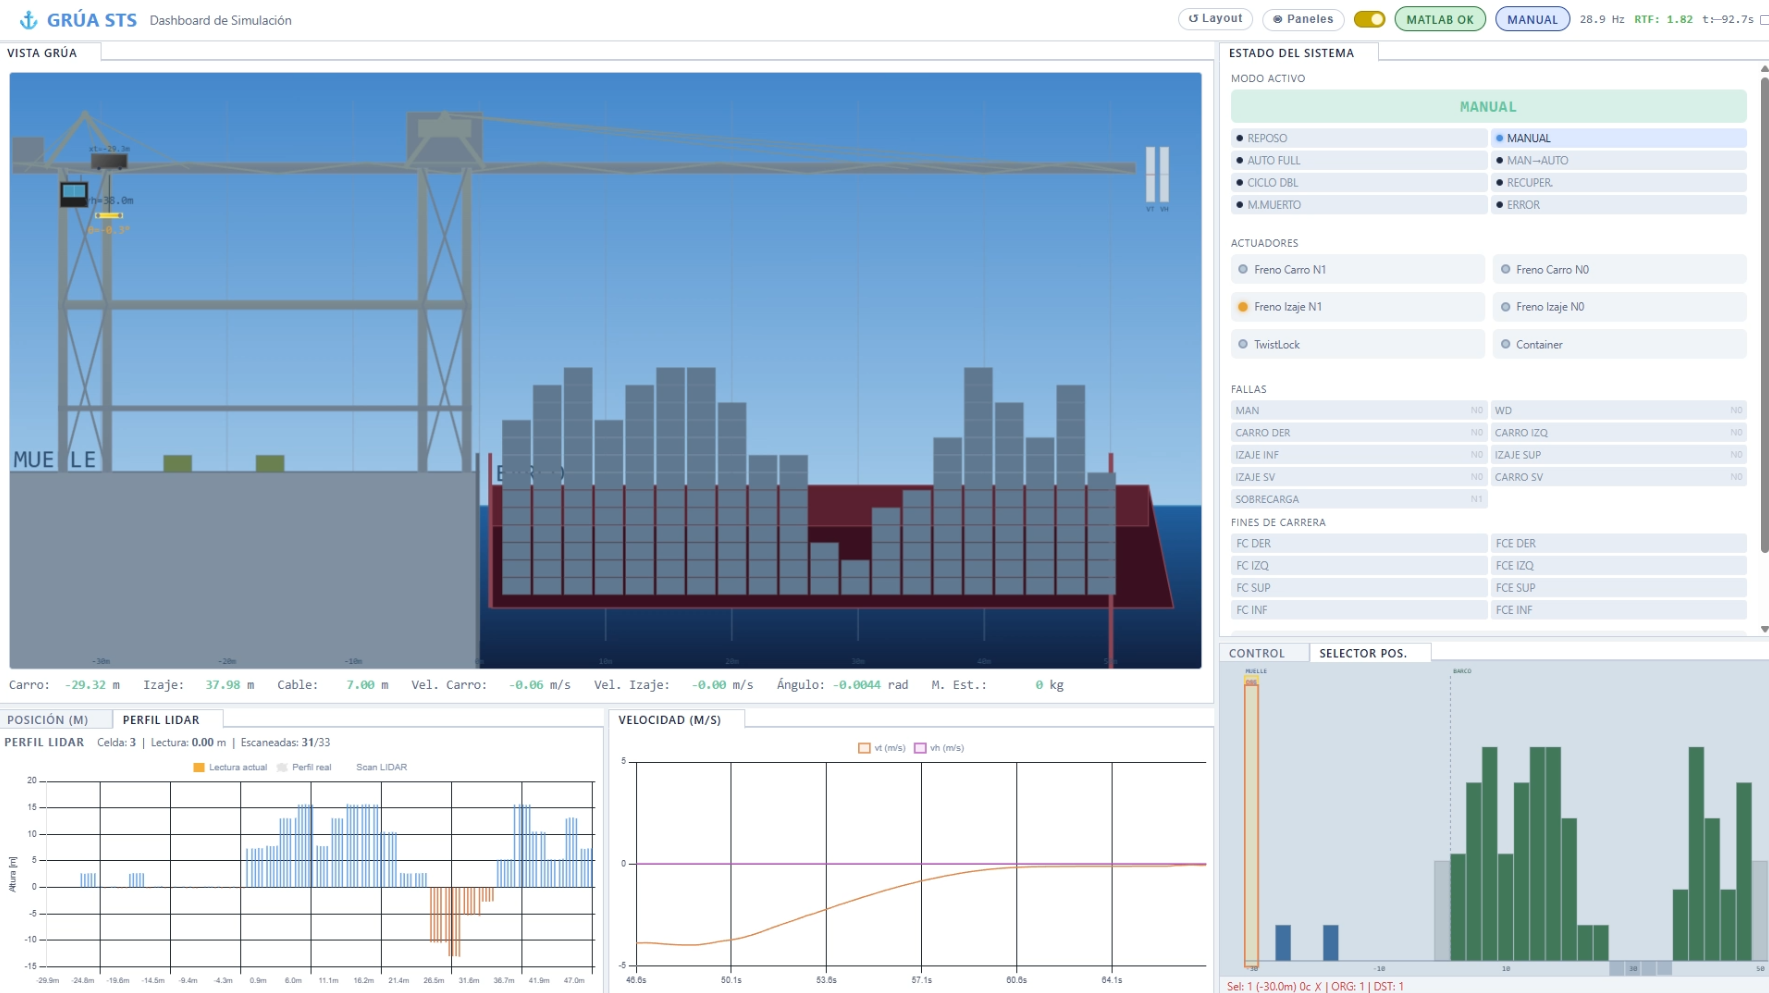
\includegraphics[width=\textwidth]{simulacion/sim_manual.png}
  
  Control del operador por joystick: traslación y elevación de la carga
\end{frame}

\begin{frame}{Modo automático: seguimiento de trayectoria}
  \centering
  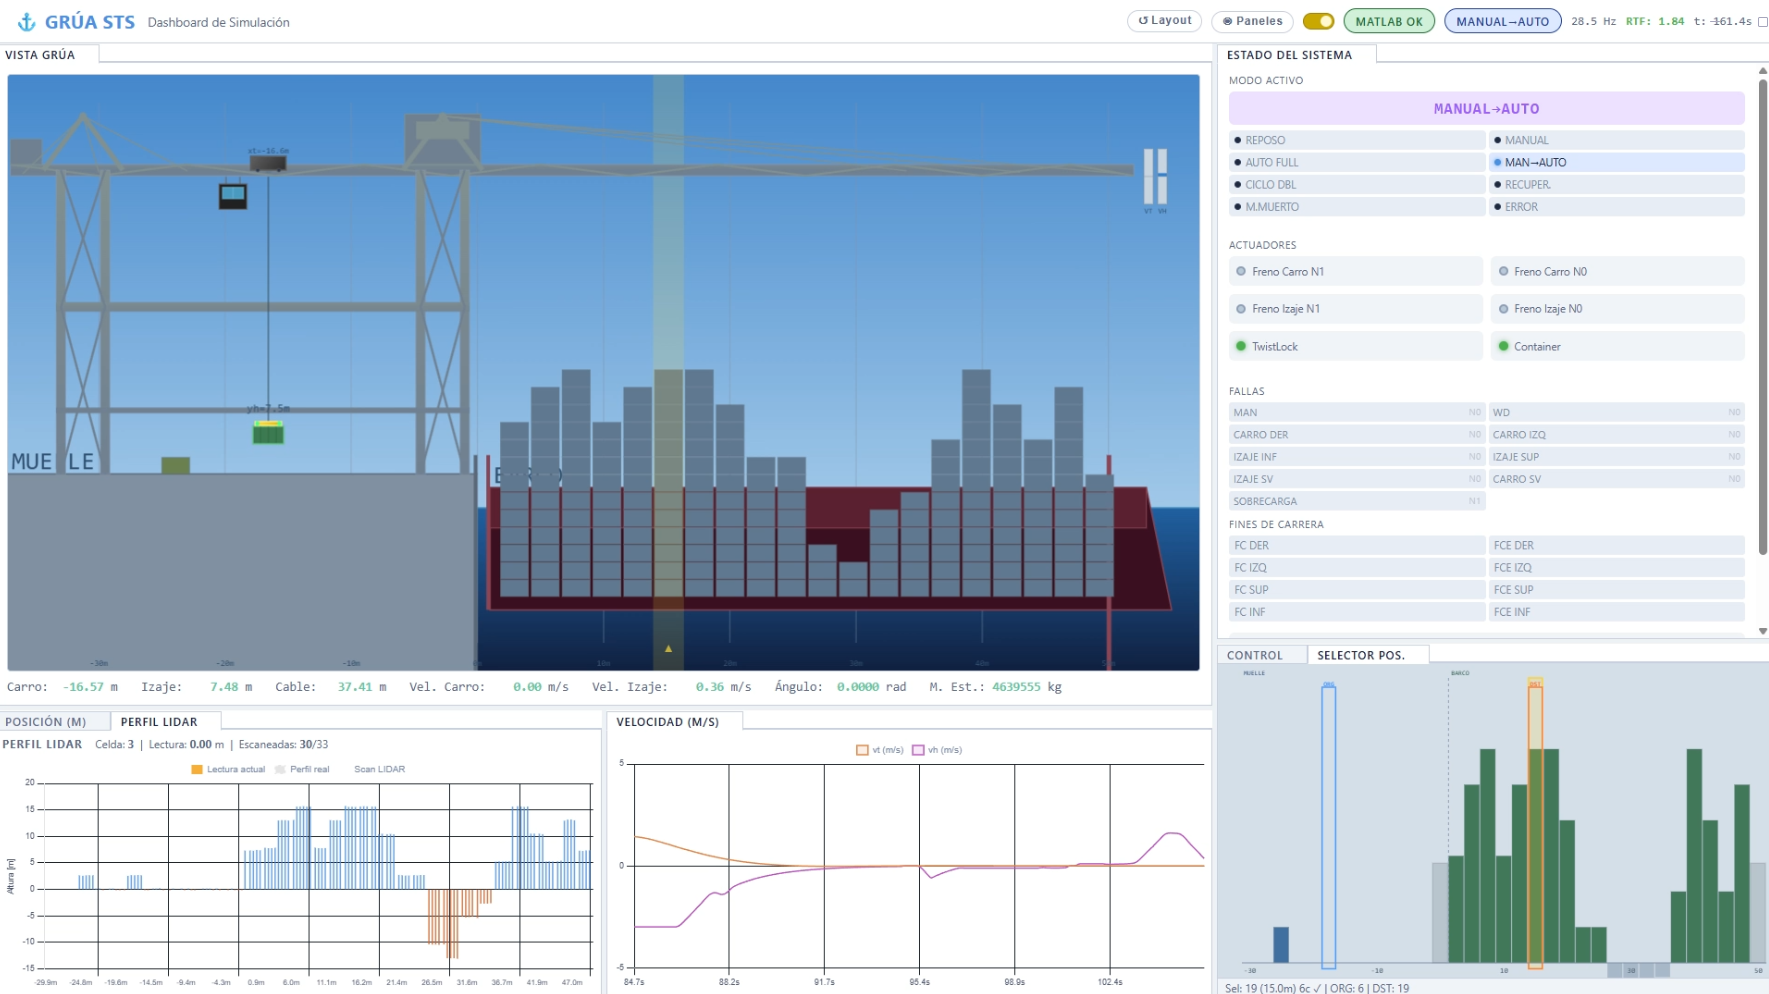
\includegraphics[width=\textwidth]{simulacion/sim_auto.png}
  
  Ejecución automática de la secuencia de operación sin intervención manual
\end{frame}

\begin{frame}{Liberación de la carga}
  \centering
  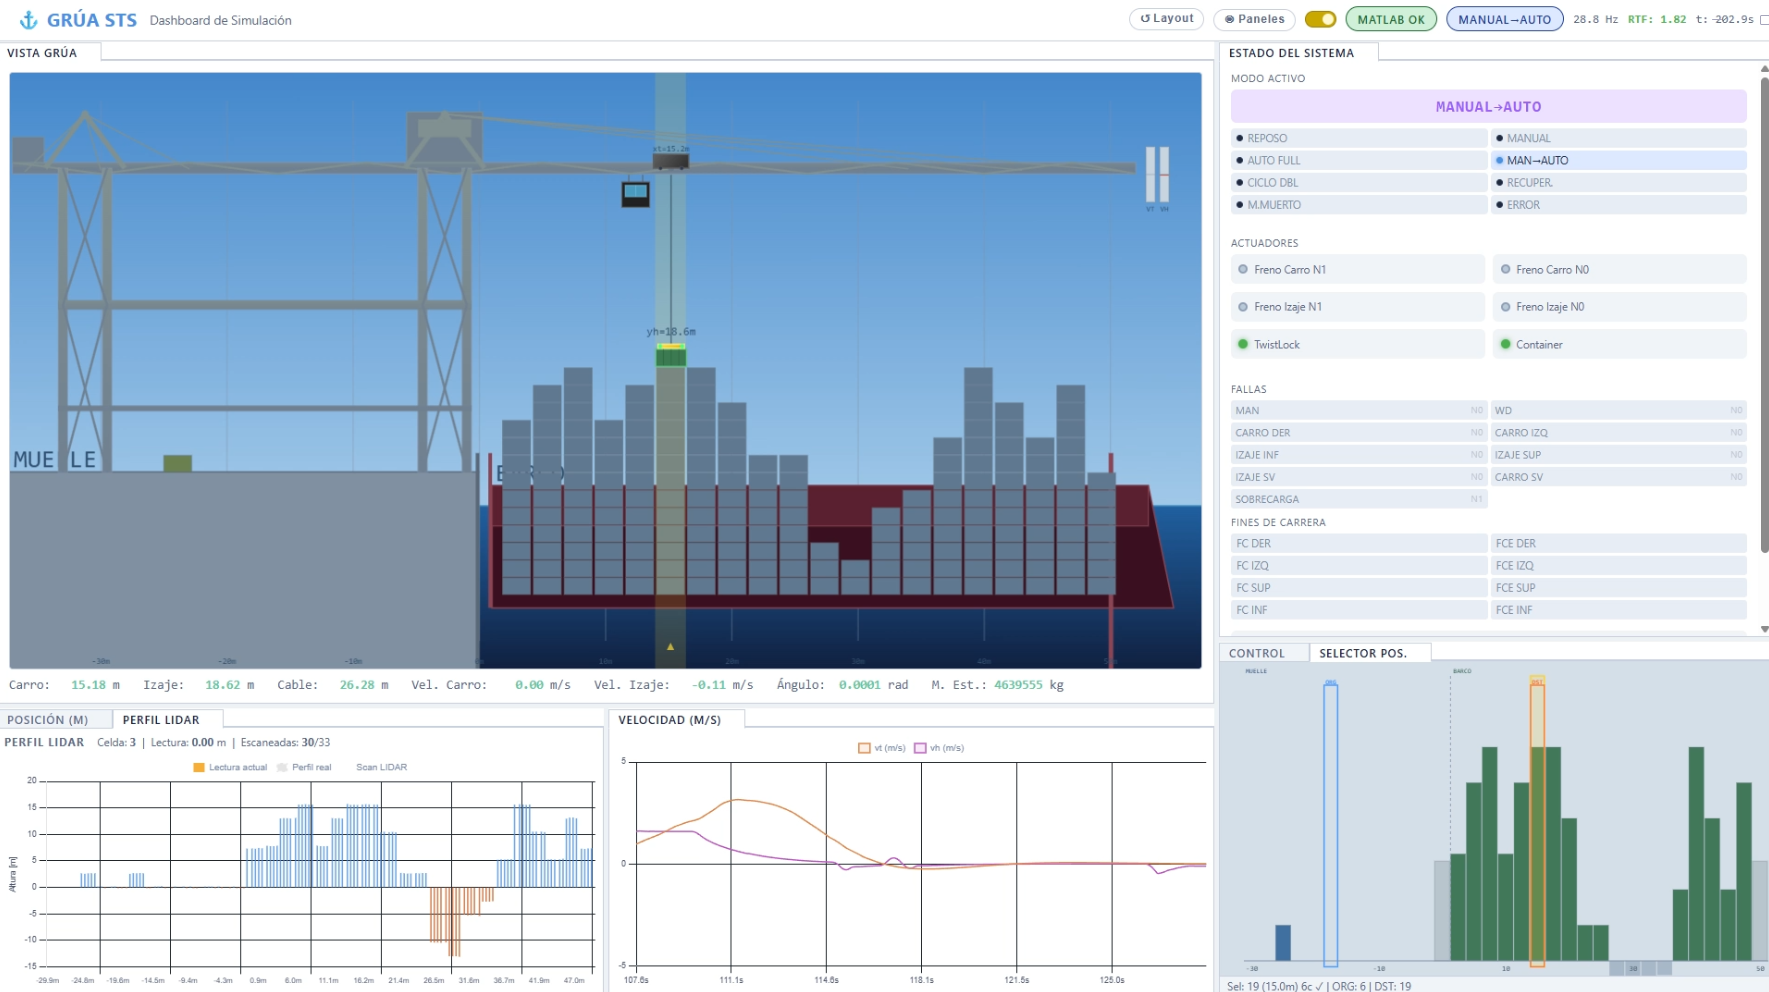
\includegraphics[width=\textwidth]{simulacion/sim_auto_leave.png}
  
  Desenganche de twistlocks y apoyado de la carga en la pila
\end{frame}

\begin{frame}{Estado de error}
  \centering
  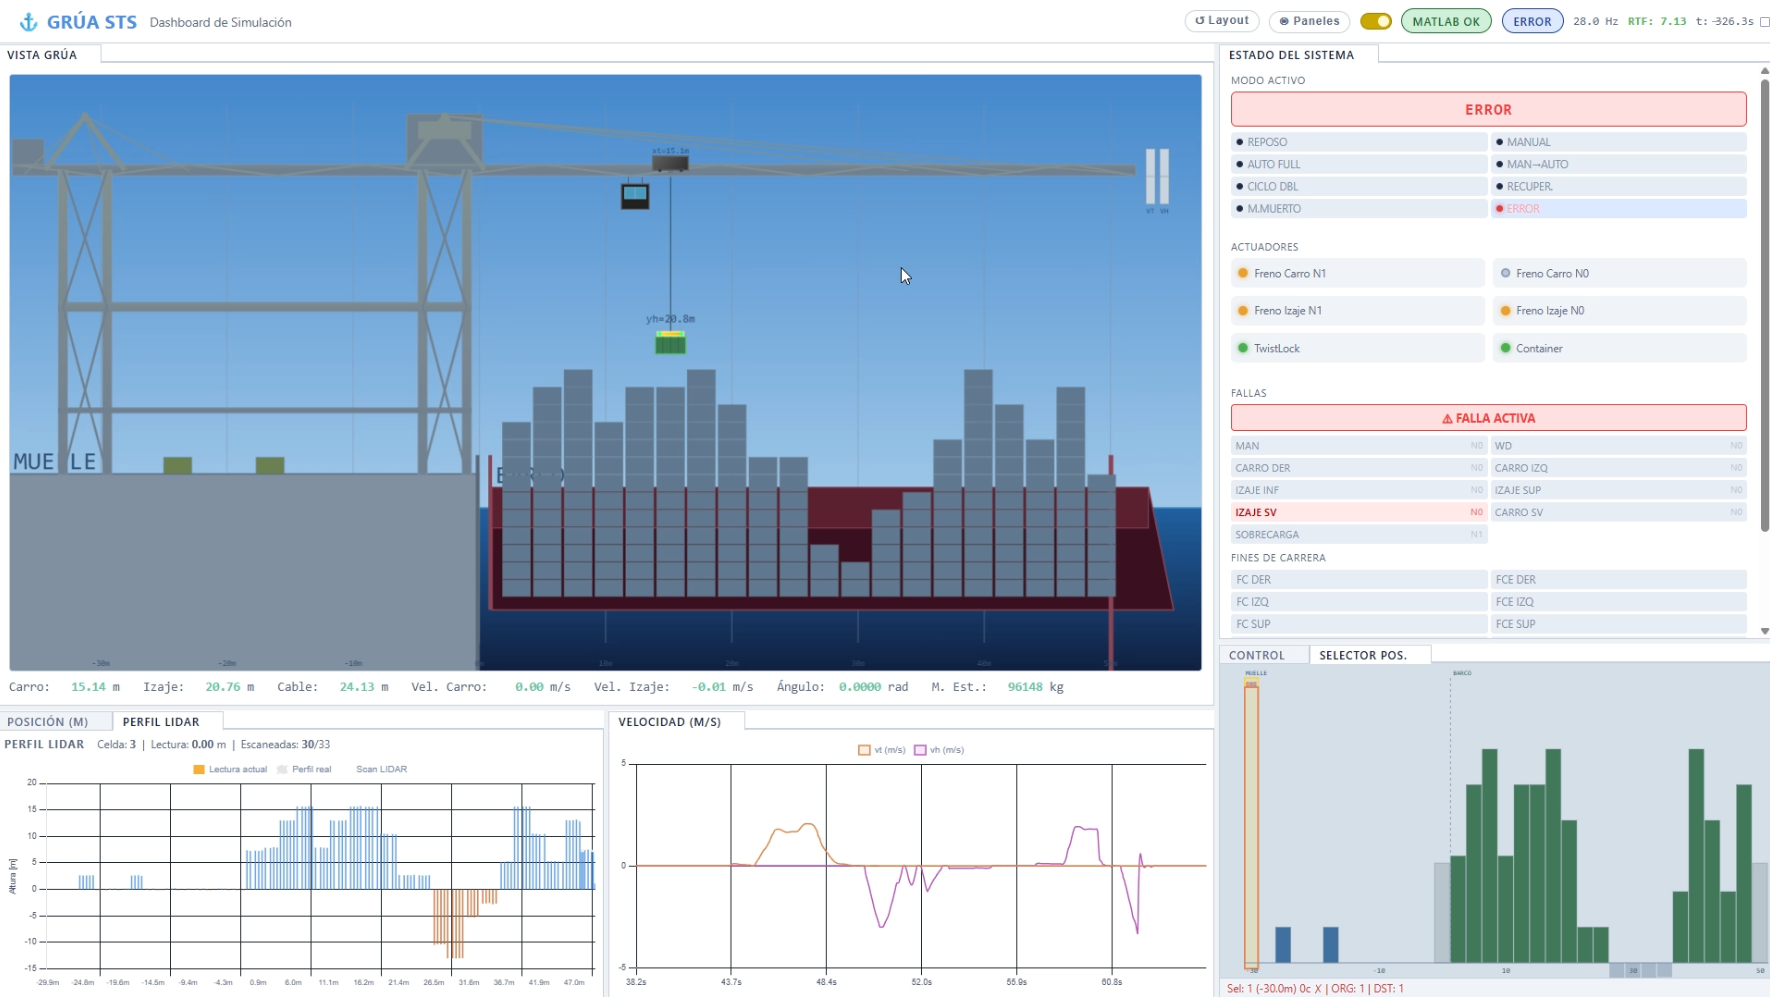
\includegraphics[width=\textwidth]{simulacion/sim_error.png}
  
  Detección de anomalía, aplicación de frenos, indicación de estado de error
\end{frame}


% \defaultmode
\section{Implementación en CODESYS}

\begin{frame}{CODESYS: codificación manual (IEC 61131)}
  \begin{columns}[T]
    \begin{column}{0.58\textwidth}
      \begin{block}{De Stateflow/Simulink a un PLC}
        Los Niveles 0 y 1 se traducen a \textbf{SFC} (Sequential Function Charts) con cálculos en
        \textbf{ST} (Structured Text); el Nivel 2 se rehace con bloques de función de Matlab
        (\textit{simil ST}).
      \end{block}
      \begin{block}{Ejecución}
        Dos POUs principales (Niveles 0 y 1) cíclicos e independientes. En el PLC virtual
        (una sola CPU) se ejecutan secuencialmente intercalados, equivalente a paralelo.
      \end{block}
    \end{column}
    \begin{column}{0.42\textwidth}
      \centering
      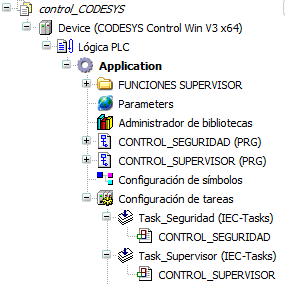
\includegraphics[width=0.85\linewidth]{codesys/arbol_codesys.png}\\
      \footnotesize Árbol de componentes del proyecto
    \end{column}
  \end{columns}
\end{frame}

\begin{frame}{Control regulatorio en simil ST: diagramas}
  Se rehace el Nivel 2 con la misma lógica pero con bloques de función de Matlab (simil ST);
  se agregan bloques \textit{Delay} para resolver loops algebraicos.
  \begin{figure}
    \centering
    \begin{subfigure}{0.49\textwidth}
      \centering
      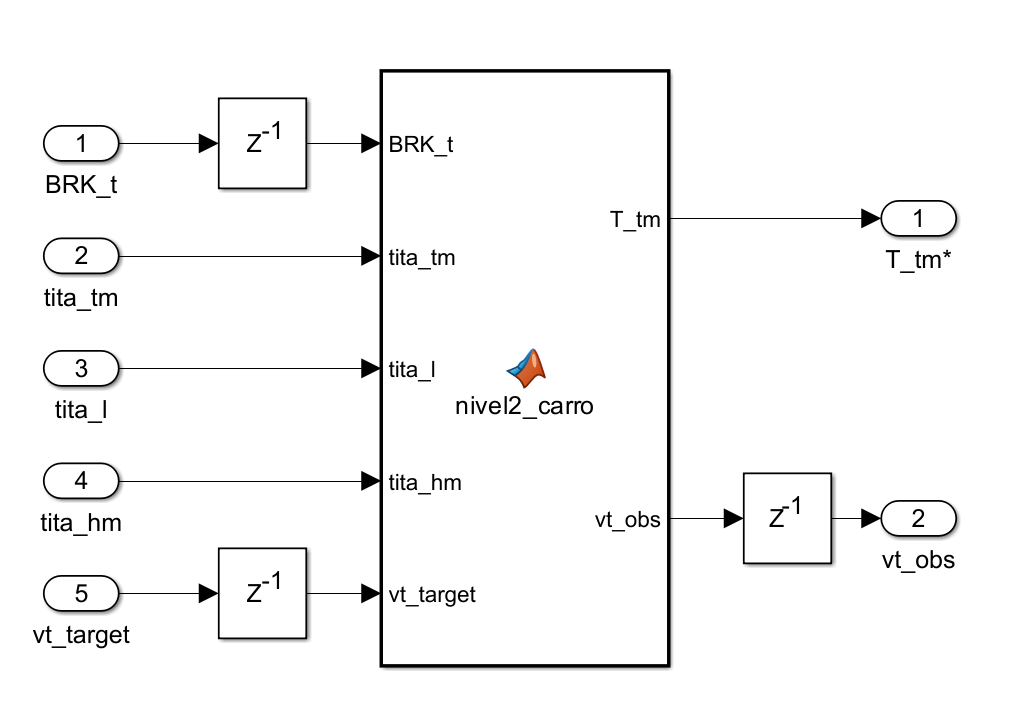
\includegraphics[width=\linewidth]{codesys/control_carro_funciones2.png}
      \caption{Control del carro}
    \end{subfigure}
    \hfill
    \begin{subfigure}{0.49\textwidth}
      \centering
      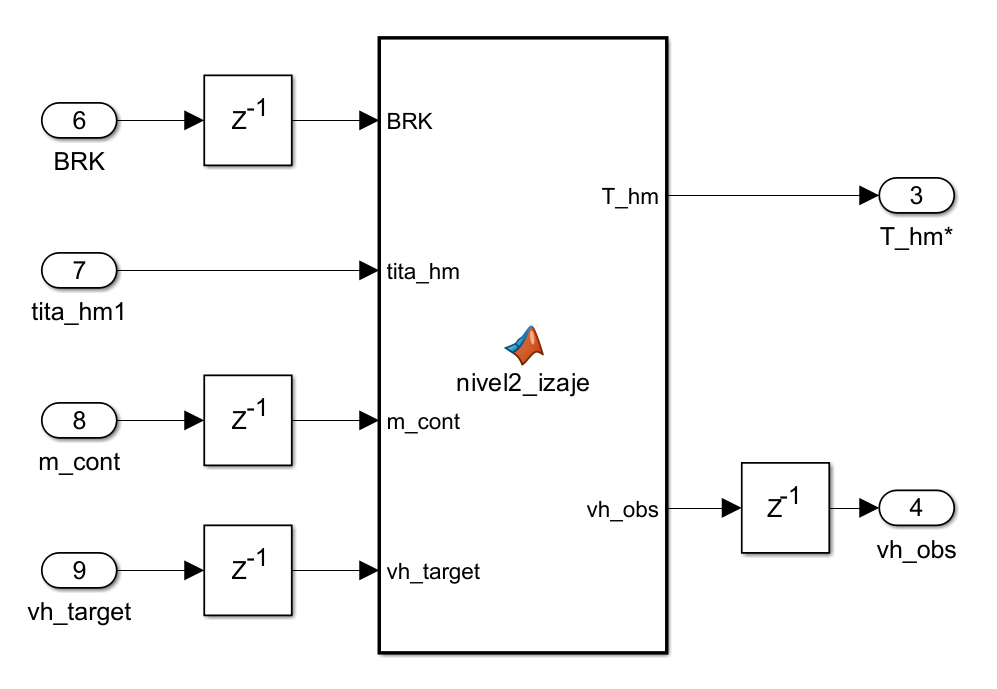
\includegraphics[width=\linewidth]{codesys/control_izaje_funciones2.png}
      \caption{Control del izaje}
    \end{subfigure}
  \end{figure}
\end{frame}

\begin{frame}{Control regulatorio en simil ST: código}
  El código de cada controlador (dentro de cada bloque de función de Matlab):
  \begin{figure}
    \centering
    \begin{subfigure}{0.42\textwidth}
      \centering
      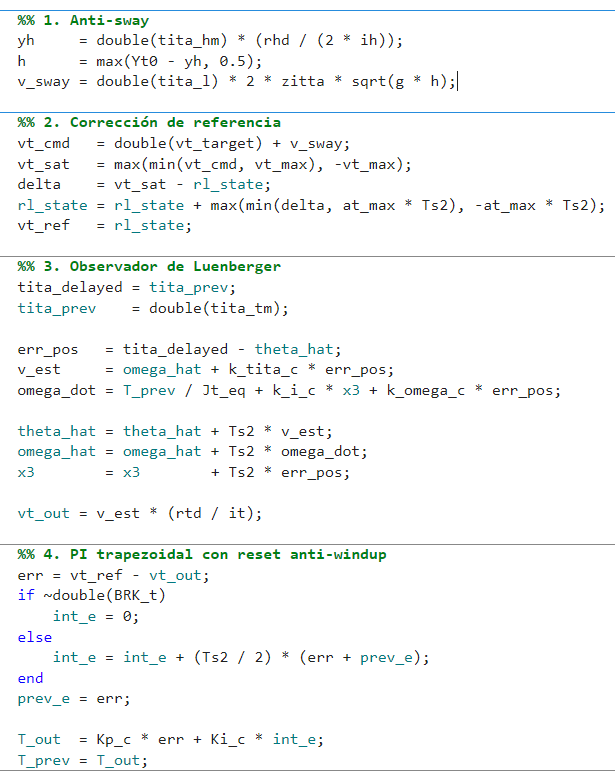
\includegraphics[width=\linewidth]{codesys/matlab_function_nivel2_carro.png}
      \caption{Control del carro (simil ST)}
    \end{subfigure}
    \hfill
    \begin{subfigure}{0.42\textwidth}
      \centering
      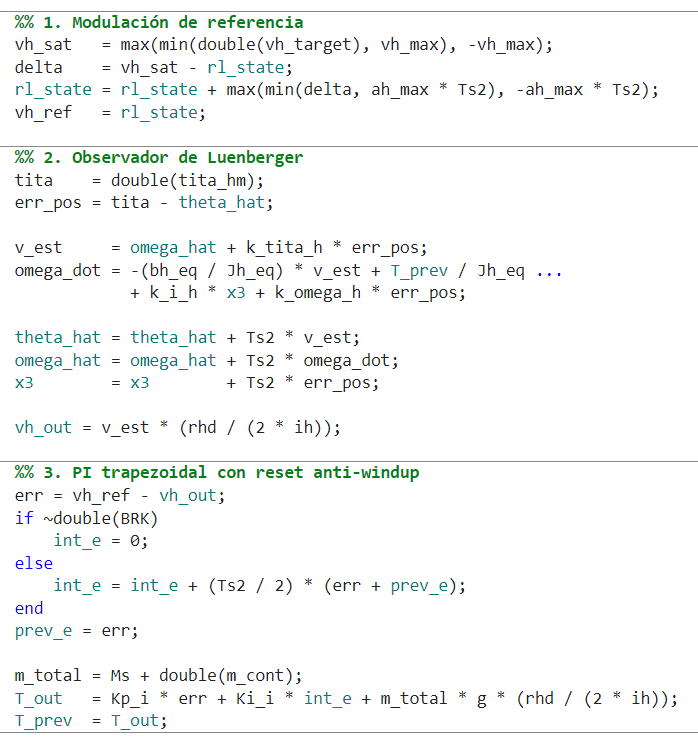
\includegraphics[width=\linewidth]{codesys/matlab_function_nivel2_izaje.png}
      \caption{Control del izaje (simil ST)}
    \end{subfigure}
  \end{figure}
\end{frame}

% \lautimode
\begin{frame}{Control supervisor: migración Stateflow → SFC}
  \centering
  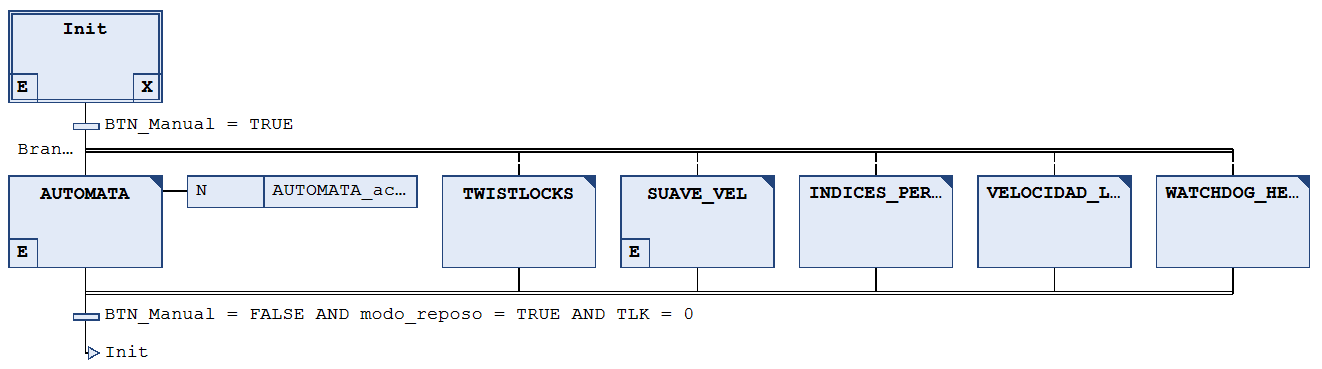
\includegraphics[width=0.95\textwidth]{codesys/codesys_supervisor11.png}
  
  Conversión de bloques Stateflow a SFC (Sequential Function Chart) manteniendo estados y transiciones
\end{frame}

\begin{frame}{Autómata principal en CODESYS}
  \centering
  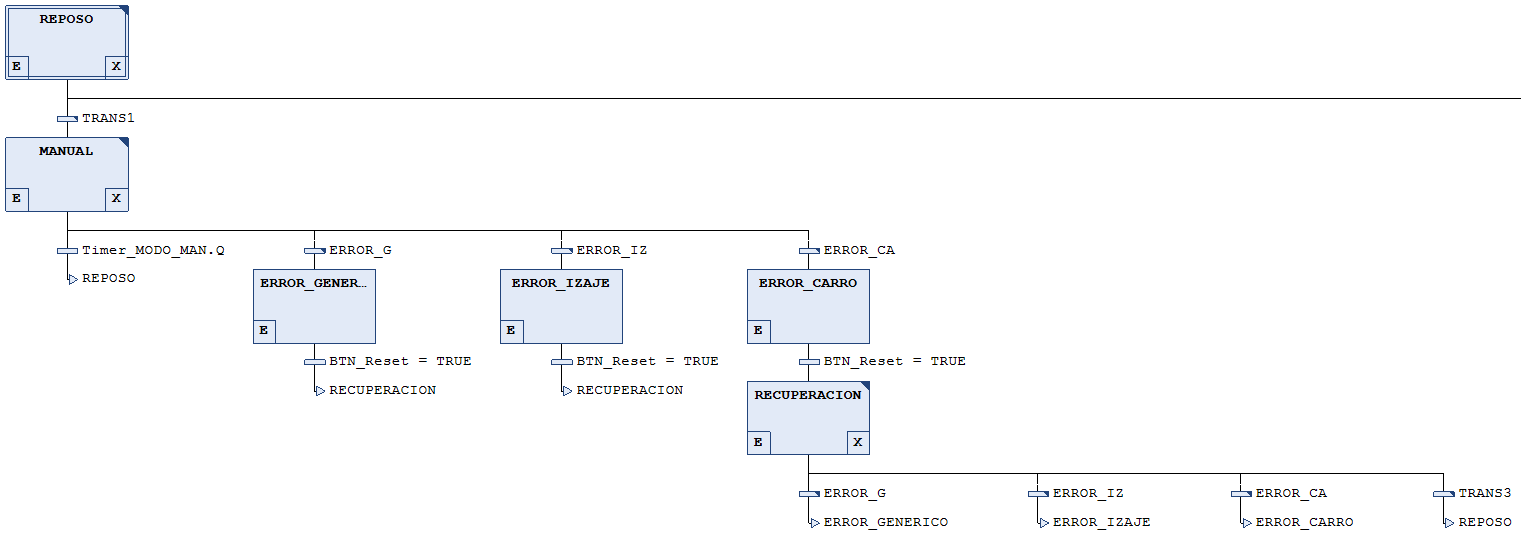
\includegraphics[width=0.95\textwidth]{codesys/codesys_supervisor12.png}
  
  \vspace{0.2cm}
  
  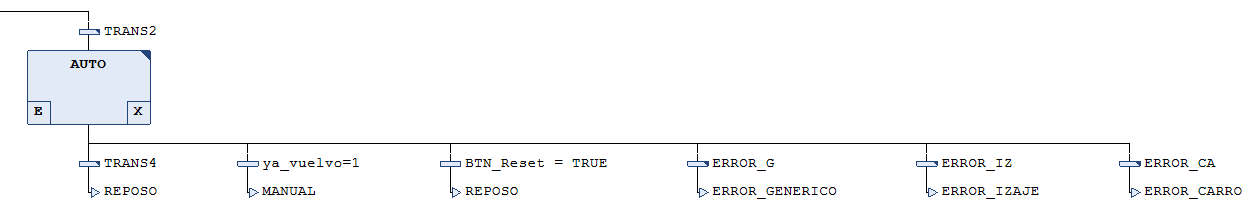
\includegraphics[width=0.95\textwidth]{codesys/codesys_supervisor13.png}
  
  Alternancia entre: REPOSO, MANUAL, AUTOMÁTICO, ERROR, RECUPERACIÓN
\end{frame}

\begin{frame}{Modo automático: adaptaciones de Stateflow a SFC}
  \centering
  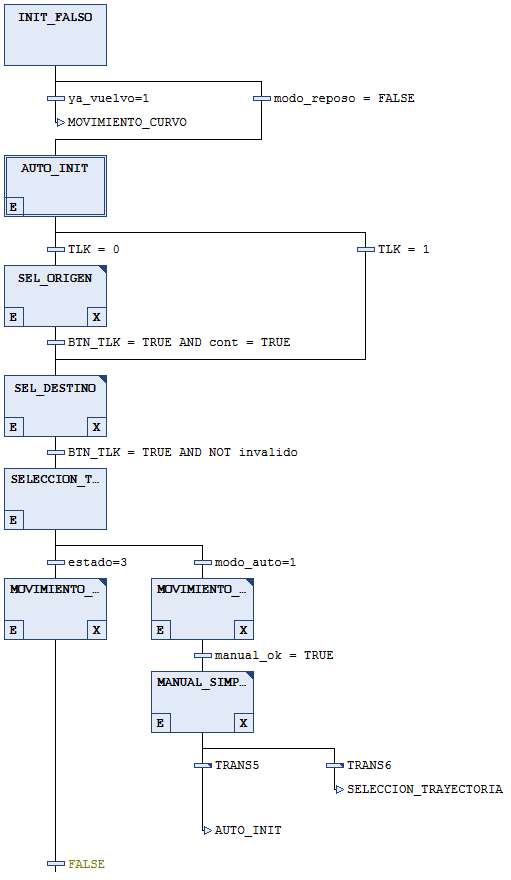
\includegraphics[width=0.7\textwidth]{codesys/codesys_supervisor15.png}
  
  Estado inicial vacío + transición FALSE para cumplir requisitos sintácticos de SFC
\end{frame}

\begin{frame}{Lógica de Twistlocks}
  \centering
  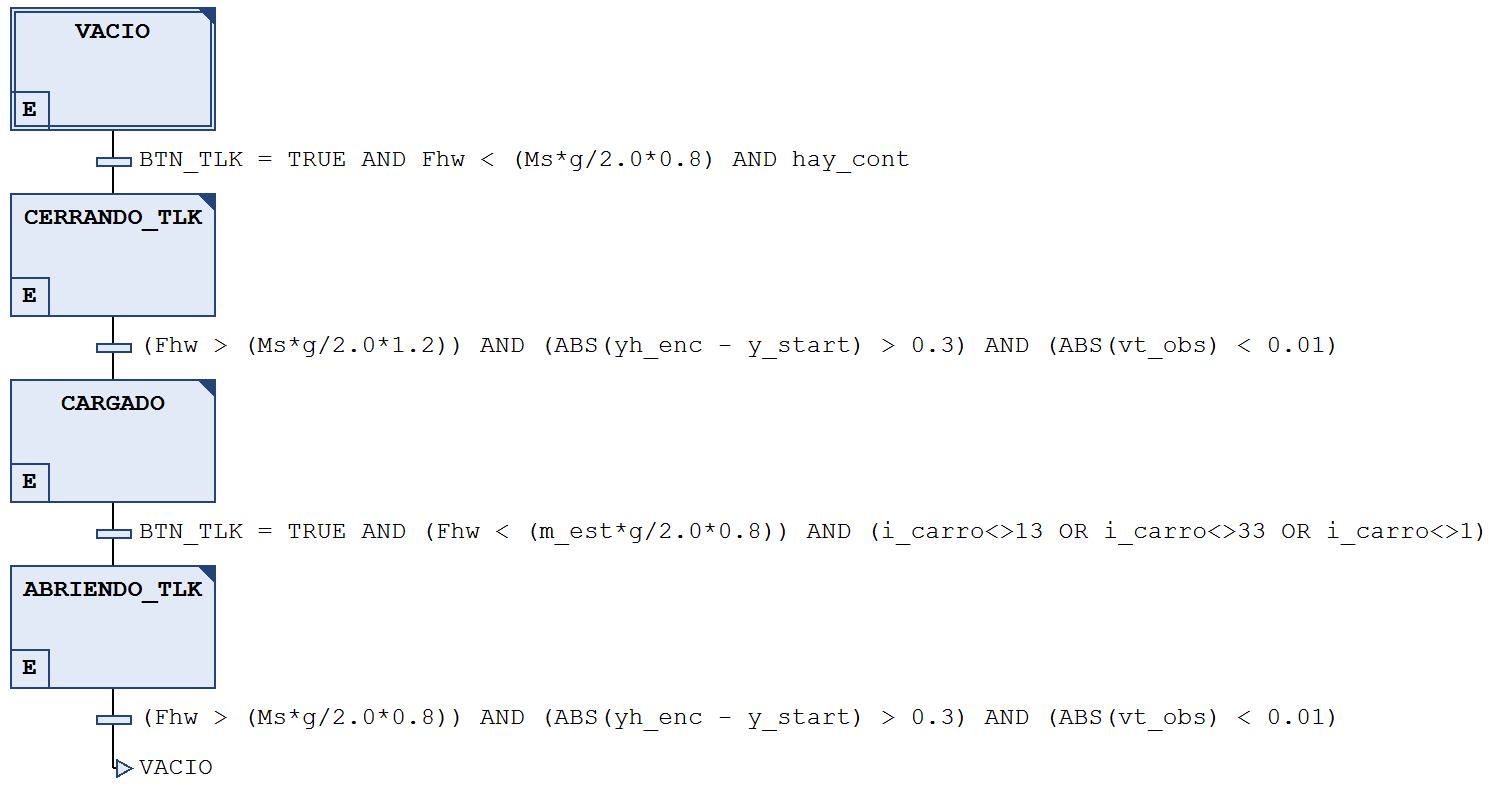
\includegraphics[width=0.85\textwidth]{codesys/codesys_supervisor4.png}
  
  SFC cíclico: últimos pasos retornan al estado inicial
\end{frame}

\begin{frame}{Cálculo de perfil e índices del muelle}
  \centering
  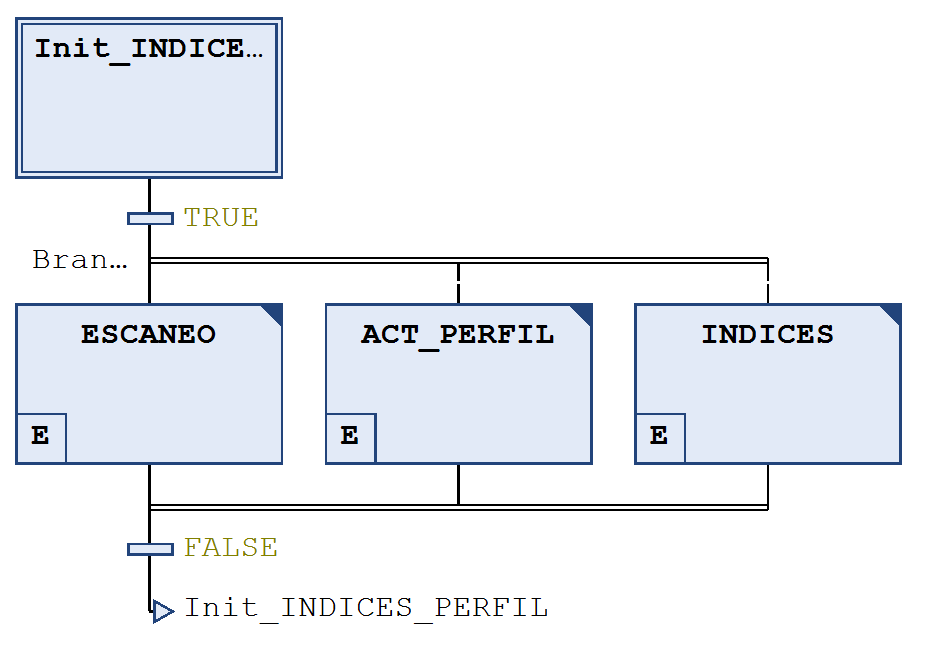
\includegraphics[width=0.8\textwidth]{codesys/codesys_supervisor14.png}
  
  Posición discreta del carro + actualización dinámica del perfil de obstáculos
\end{frame}

\begin{frame}{Bloques complementarios}
  \begin{block}{Suavizado de velocidad}
    Implementado en ST: suaviza referencias de velocidad
  \end{block}
  
  \begin{block}{Velocidad límites}
    Implementado en ST: aplicación de límites de velocidad por zona
  \end{block}
  
  \begin{block}{Watchdog heartbeat}
    Implementado en ST: monitoreo de comunicación con sistema de control
  \end{block}
\end{frame}

\subsection{Comunicación OPC-UA Simulink/CODESYS}

\begin{frame}{Protocolo OPC-UA para comunicación Simulink/CODESYS}
  \centering
  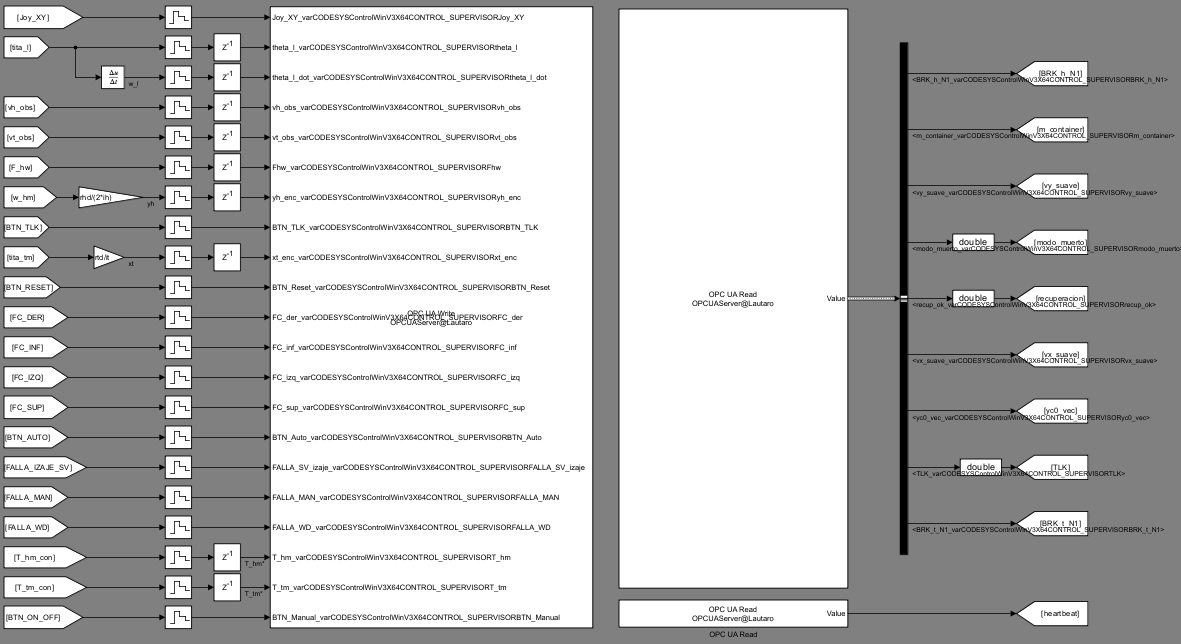
\includegraphics[width=0.85\textwidth]{codesys/opc_ua_1.png}
  
  Servidor OPC-UA en CODESYS con cliente en Matlab R2025b. Configuración: \textit{User allow anonymous} para lectura/escritura en tiempo real
\end{frame}

\begin{frame}{Bloques de comunicación: control de protección}
  \centering
  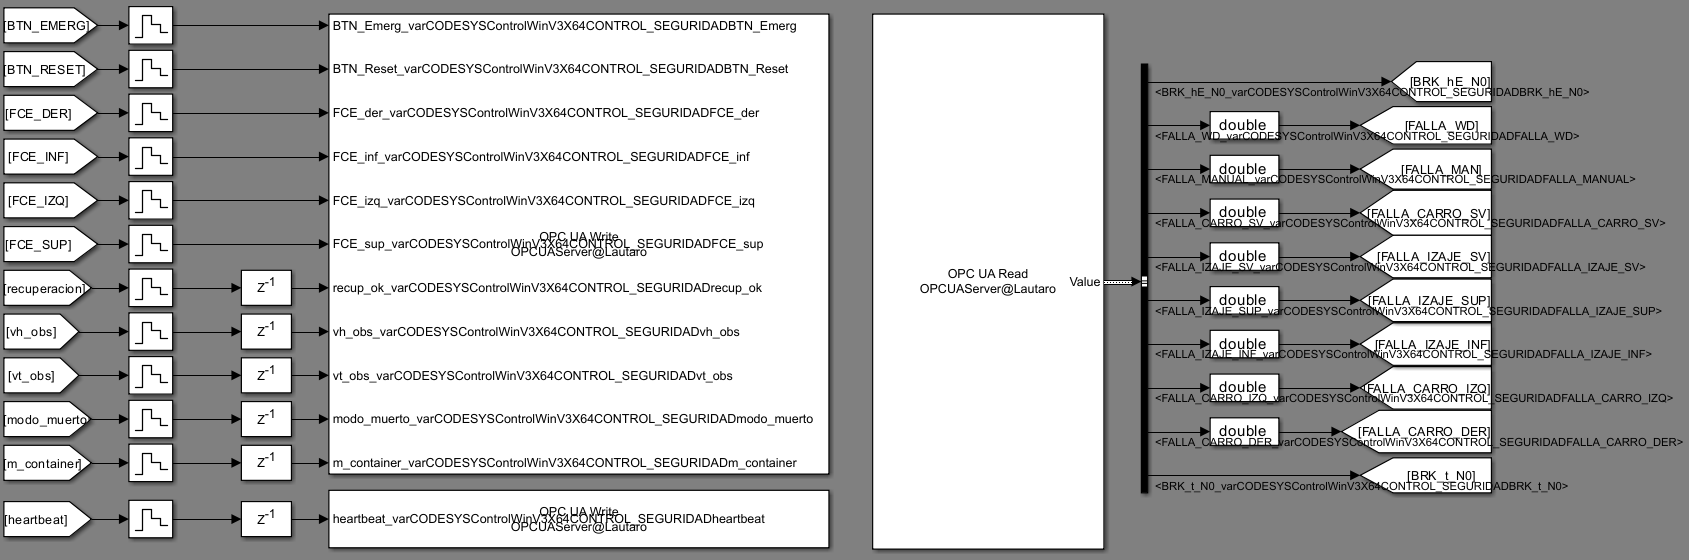
\includegraphics[width=0.9\textwidth]{codesys/opc_ua_0.png}
  
  Lectura/escritura de variables de protección (Nivel 0) a través de OPC-UA
\end{frame}

\begin{frame}{Desafío: retardo de comunicación}
  \begin{block}{Problema}
    OPC es protocolo TCP/IP diseñado para SCADA (retardos $\geq 500$ ms), no para control tiempo real
  \end{block}
  
  \begin{block}{Solución implementada}
    Bloques de comunicación con tiempos de muestreo diferenciados:
    \begin{itemize}
      \item Control supervisor y protección: $500$ ms
      \item Watchdog heartbeat: $20$ ms (tiempo original)
    \end{itemize}
    Reduce carga en red permitiendo Simulink correr a $1$s por segundo de simulación
  \end{block}
\end{frame}

\begin{frame}{Simulación con OPC-UA en funcionamiento}
  \centering
  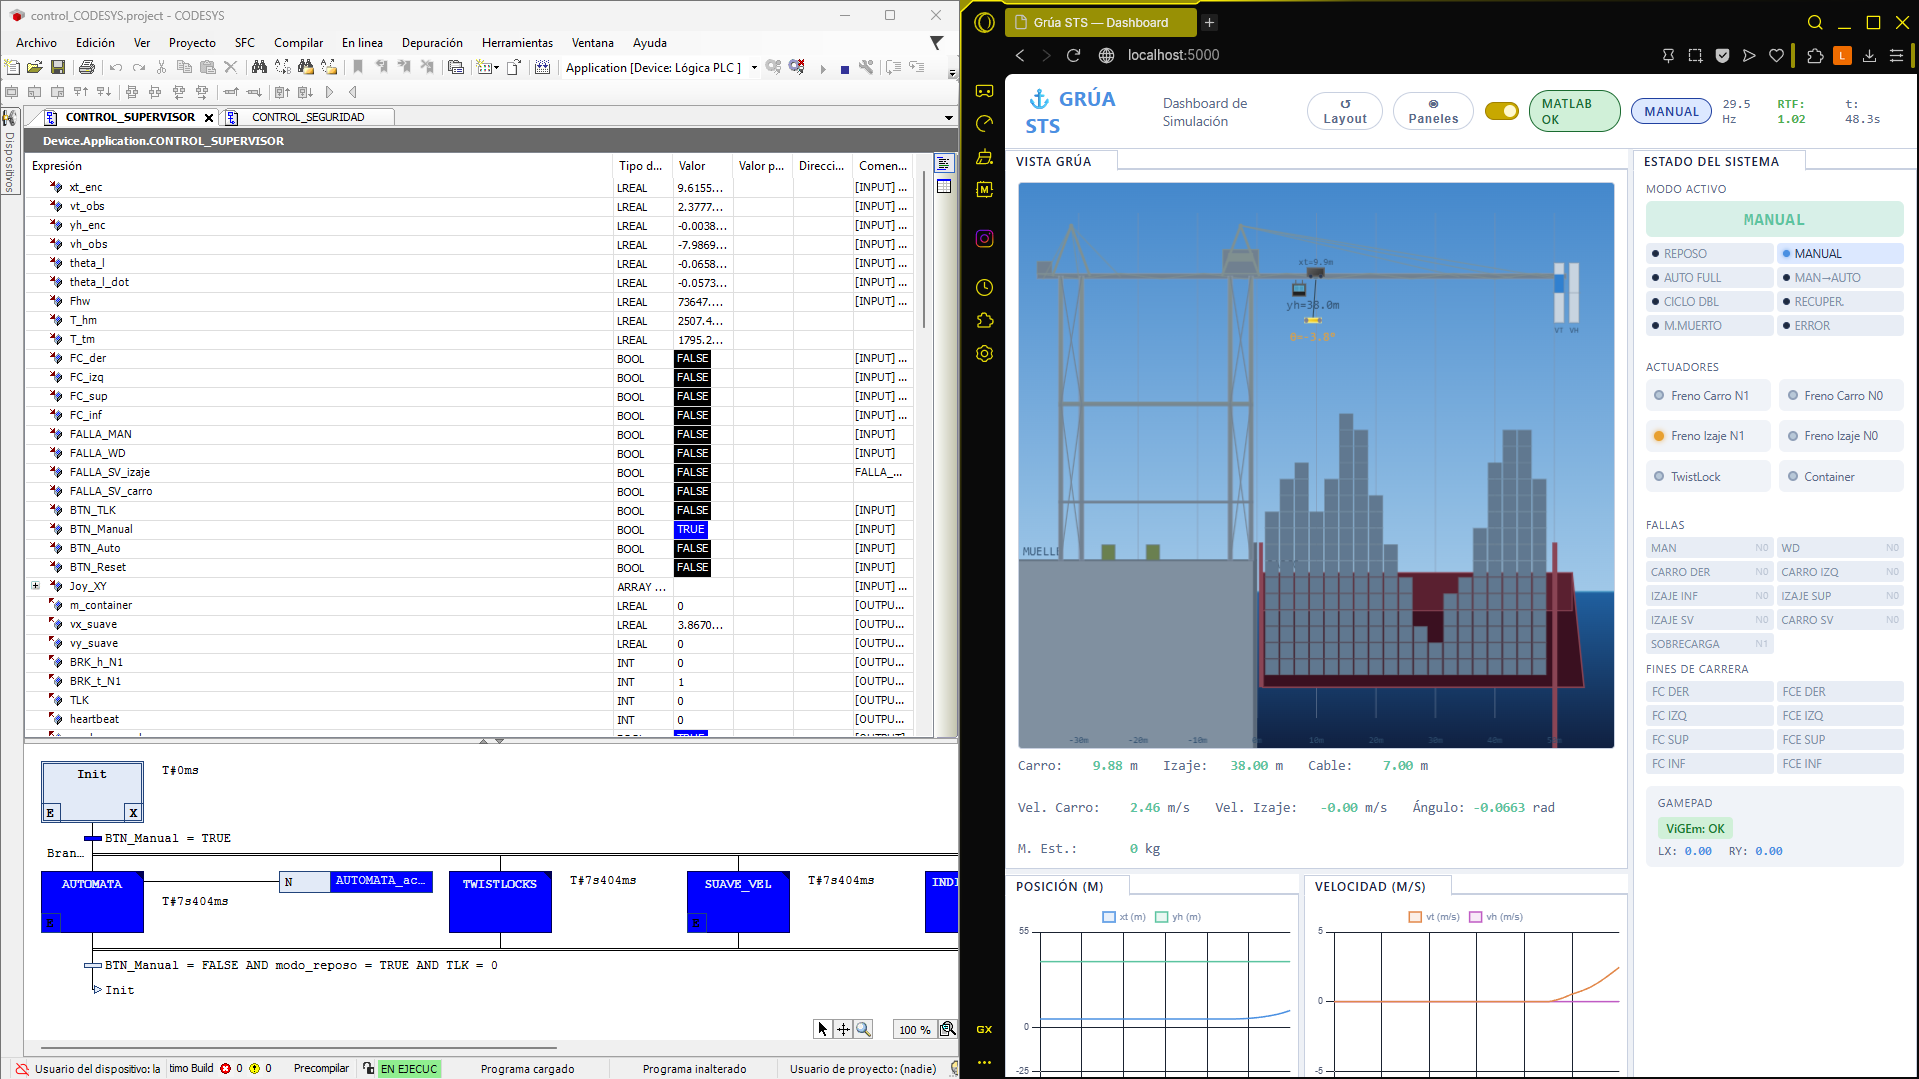
\includegraphics[width=0.9\textwidth]{codesys/codesys_interfaz.png}
  
  Mejora significativa en fluidez de simulación con comunicación OPC-UA. Controlador responde de forma equivalente al modelo en Simulink
\end{frame}


% \defaultmode
% \section{Simulación y resultados}

\begin{frame}{Visualización: animación 2D en tiempo real}
  \begin{columns}[T]
    \begin{column}{0.45\textwidth}
      \begin{itemize}
        \item Bloque \textbf{UDP} envía el estado de la planta a un programa en \textbf{Python}.
        \item Animación 2D en el navegador: grúa, contenedores, barco y parámetros clave.
        \item Permite \textbf{monitorear y operar} la grúa en los distintos modos.
      \end{itemize}
    \end{column}
    \begin{column}{0.55\textwidth}
      \centering
      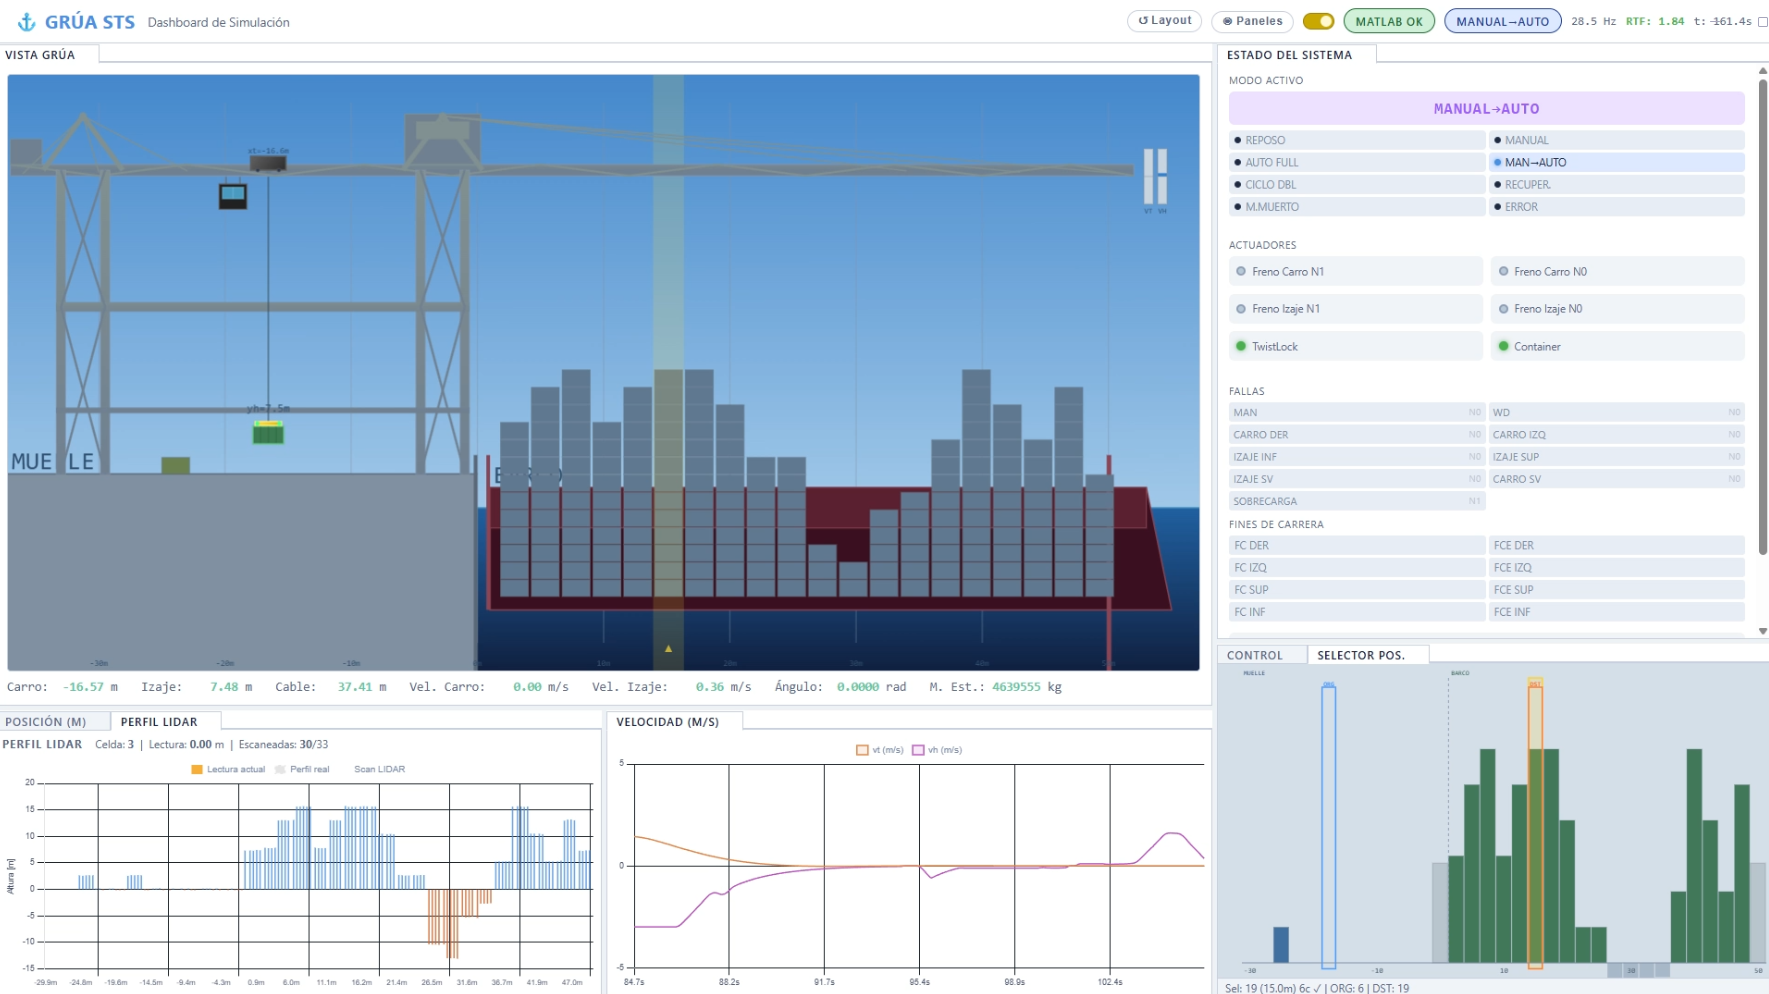
\includegraphics[width=\linewidth]{simulacion/sim_auto.png}
    \end{column}
  \end{columns}
\end{frame}

\begin{frame}{Modos de operación verificados}
  \begin{columns}[T]
    \begin{column}{0.5\textwidth}
      \centering
      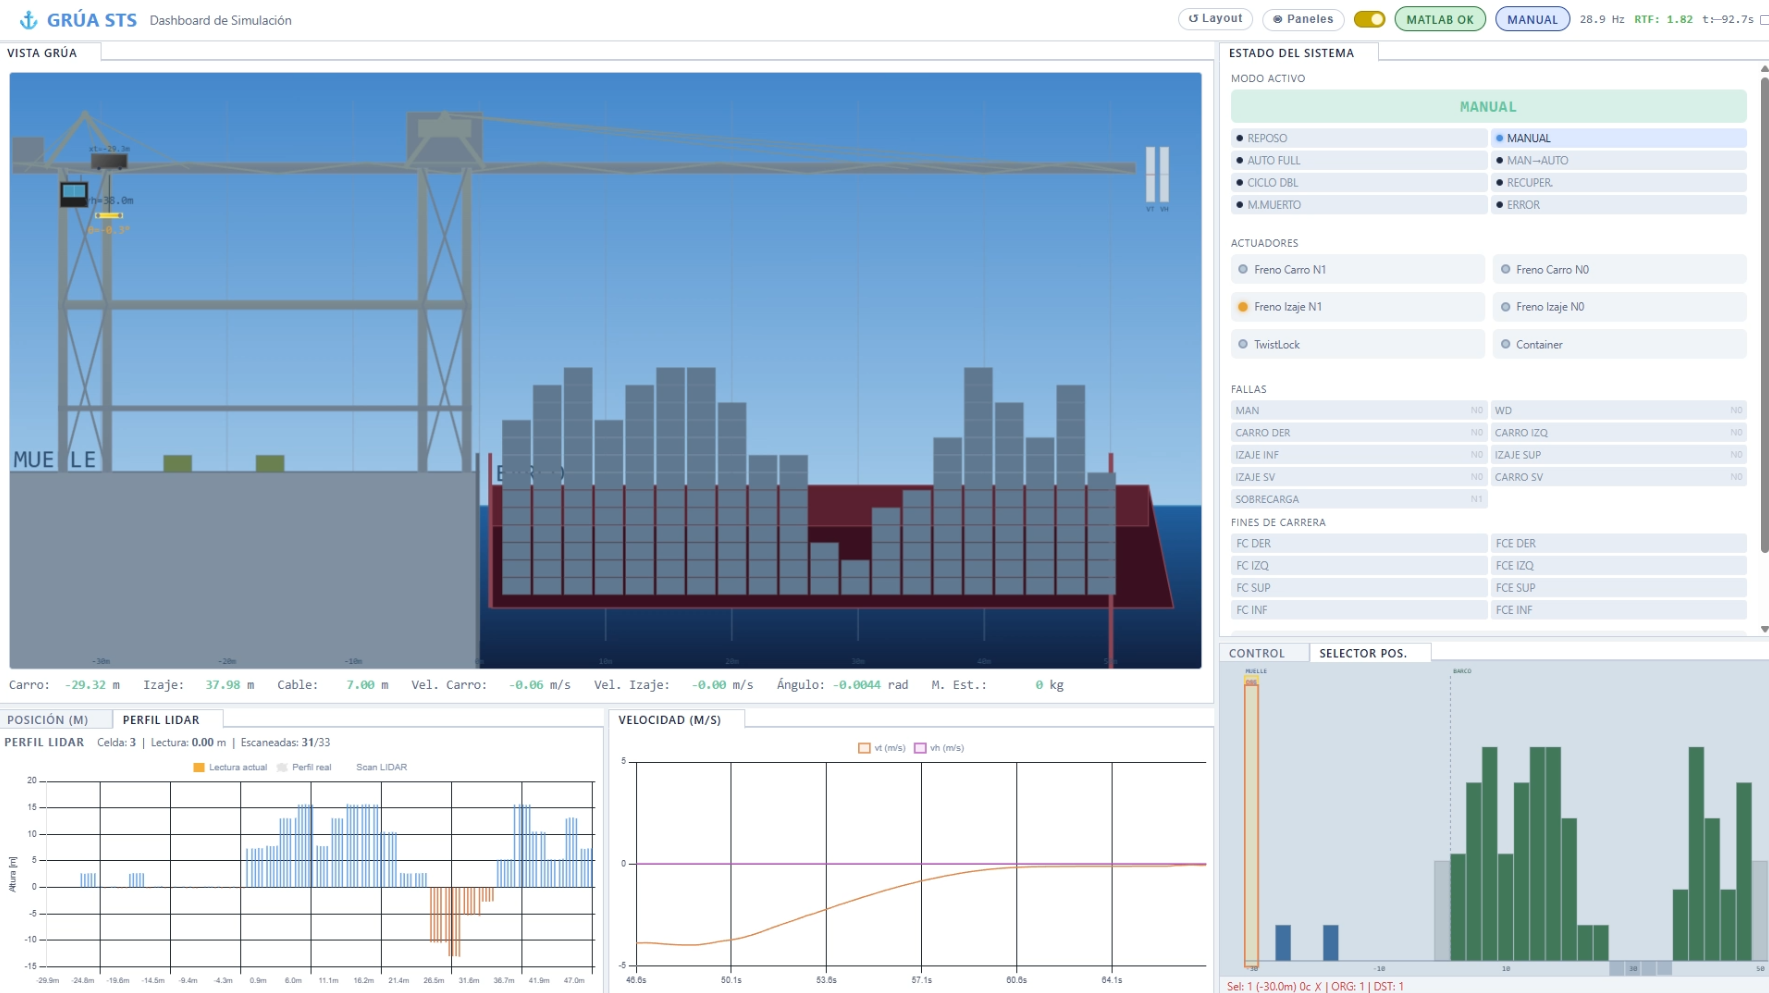
\includegraphics[width=\linewidth]{simulacion/sim_manual.png}\\
      \footnotesize Modo manual
    \end{column}
    \begin{column}{0.5\textwidth}
      \centering
      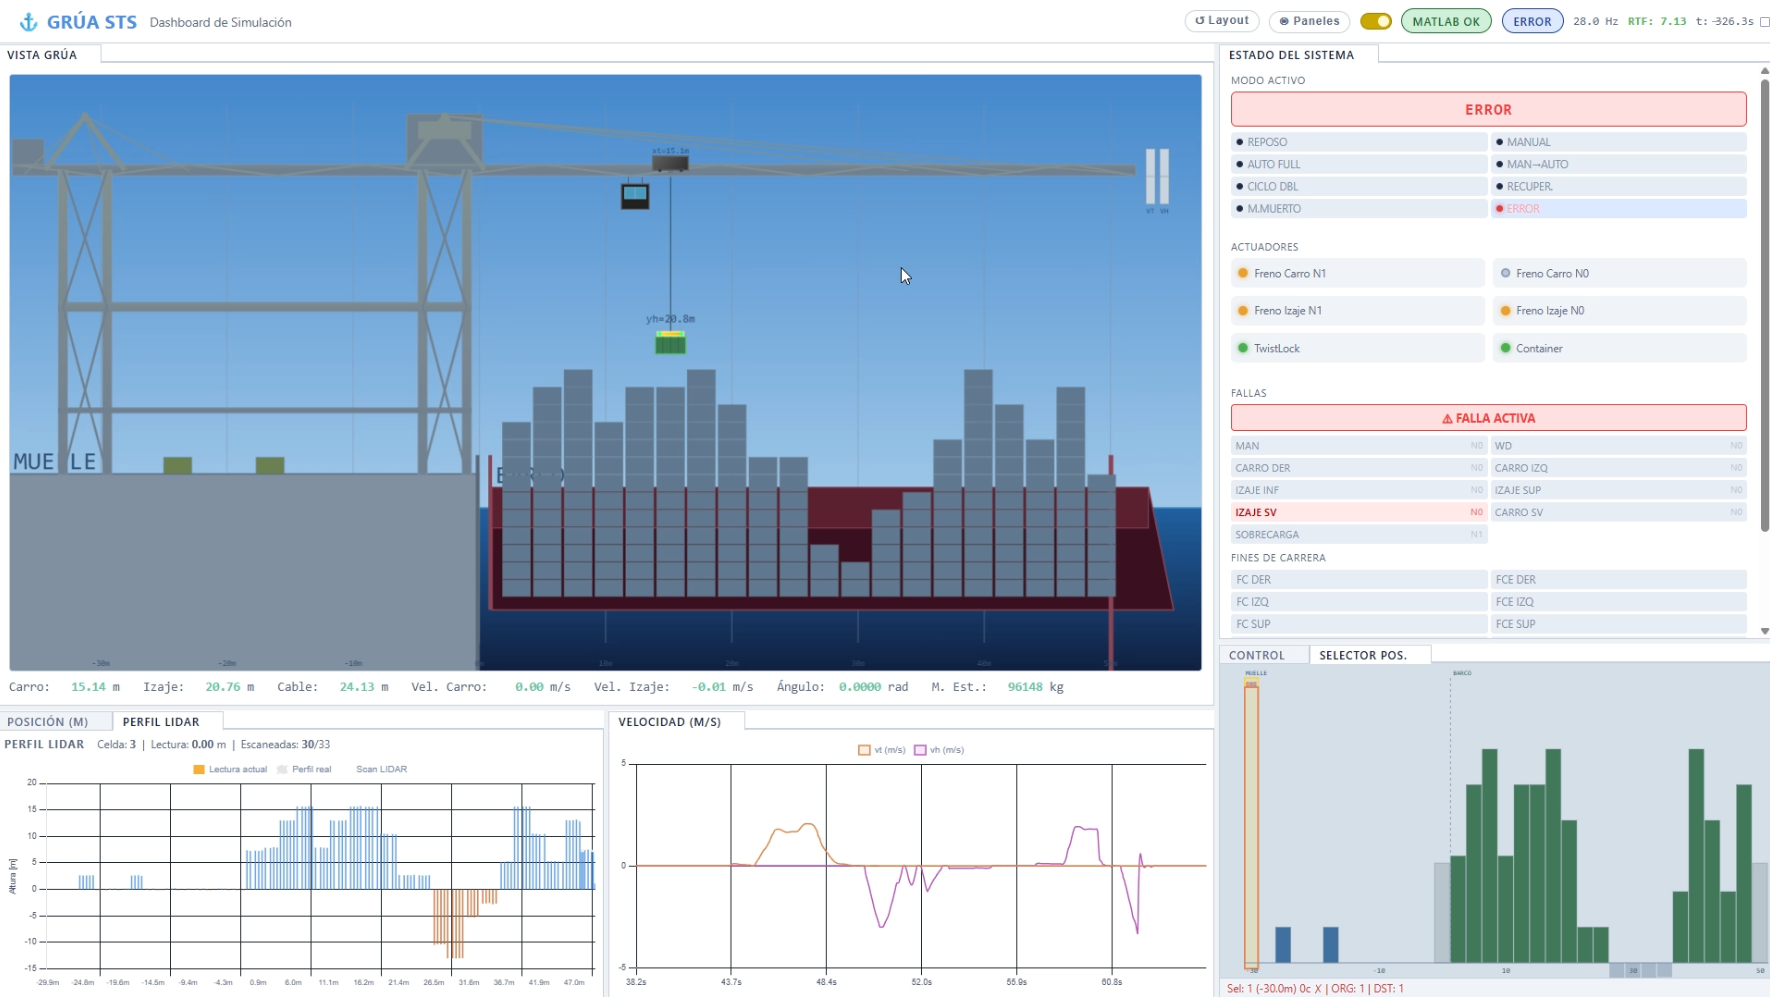
\includegraphics[width=\linewidth]{simulacion/sim_error.png}\\
      \footnotesize Estado de error (parada de emergencia)
    \end{column}
  \end{columns}
\end{frame}

\begin{frame}{Desempeño}
  \begin{itemize}
    \item Ciclos completos de carga/descarga \textbf{autónomos} y \textbf{sin colisiones}.
    \item Seguimiento de velocidad sin sobrepaso; balanceo residual despreciable al posicionar.
    \item Transferencia manual$\leftrightarrow$automático \textbf{sin golpe} (\textit{bumpless}).
    \item Estimación de masa $\Rightarrow$ velocidad a \textbf{potencia constante} y bloqueo por
          sobrecarga.
    \item Objetivo de productividad: \textbf{$\geq 30$ contenedores/hora}.
  \end{itemize}
\end{frame}

\section{Generación automática de código ST}

\begin{frame}{Generación automática de código ST}
  \begin{block}{Herramienta: Simulink PLC Coder}
    Traduce automáticamente los Statecharts a \textbf{Texto Estructurado} (ST, norma IEC 61131-3).
  \end{block}

  \begin{block}{Estructura del código generado}
    Autómata \textbf{plano y monolítico}: un \texttt{CASE} global sobre la variable de estado, con
    una densa red de \texttt{IF/ELSIF} anidados para resolver transiciones y acciones.
  \end{block}

  \begin{alertblock}{Manual (SFC) vs. autogenerado (ST)}
    \begin{itemize}
      \item \textbf{Eficiencia / CPU}: comparable (el compilador del PLC optimiza ambos).
      \item \textbf{Legibilidad y diagnóstico}: el ST autogenerado \textbf{carece de trazabilidad
            visual} $\Rightarrow$ difícil de interpretar en planta.
    \end{itemize}
    Por eso se optó por \textbf{SFC manual} para la arquitectura y ST sólo para los cálculos.
  \end{alertblock}
\end{frame}

\begin{frame}{Fragmento de código ST autogenerado (PLC Coder)}
  \centering
  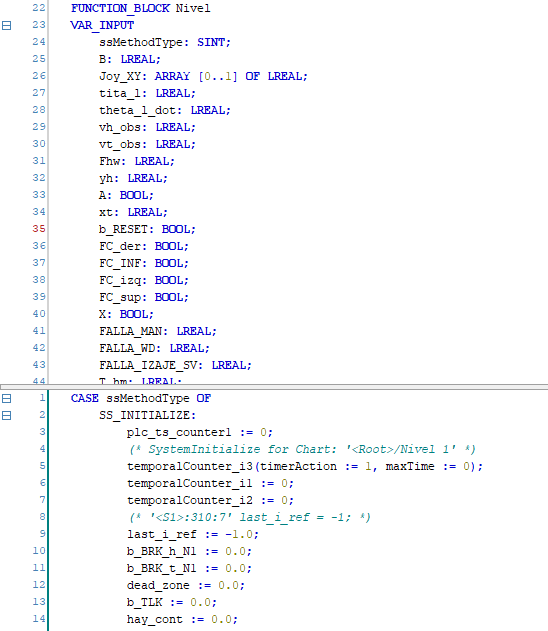
\includegraphics[width=\linewidth,height=0.82\textheight,keepaspectratio]{codesys/st_generado.png}
\end{frame}

\section{Conclusiones}

\begin{frame}{Conclusiones: logros por nivel}
  \small
  \begin{itemize}
    \item \textbf{Nivel 2 --- regulatorio:}
      \begin{itemize}
        \item Seguimiento de velocidad preciso y \textbf{sin sobrepaso} en ambos ejes.
        \item El izaje sostiene el peso \textbf{sin caída} de velocidad (compensación de gravedad).
        \item El observador entrega una velocidad estimada limpia, sin ruido de derivar el encoder.
        \item El \textit{anti-sway} reduce el balanceo a valores despreciables al finalizar la
              maniobra $\Rightarrow$ apilado preciso.
      \end{itemize}
    \item \textbf{Nivel 1 --- supervisor:}
      \begin{itemize}
        \item Ciclos completos de carga/descarga \textbf{autónomos}, sin colisionar con la pila
              (LIDAR).
        \item La estimación de masa y el límite por curva de potencia \textbf{impiden la sobrecarga}.
        \item El suavizado y los límites suaves logran trayectorias fluidas que nunca alcanzan los
              finales de carrera de forma abrupta.
      \end{itemize}
    \item \textbf{Nivel 0 --- protección:}
      \begin{itemize}
        \item Ante las fallas inducidas (sobrevelocidad, FC de emergencia, parada manual, pérdida
              del \textit{heartbeat}) lleva el sistema a un estado seguro.
        \item Detiene \textbf{sólo el eje afectado}; la grúa nunca sigue operando con un comando
              desactualizado.
      \end{itemize}
  \end{itemize}
\end{frame}

\begin{frame}{Validación e implementación}
  \begin{itemize}
    \item Comportamiento validado en \textbf{simulación}, apoyada en una animación 2D en tiempo
          real que muestra la operación en los distintos modos.
    \item La lógica de control se trasladó a un PLC virtual en \textbf{CODESYS} (SFC + texto
          estructurado).
    \item Co-simulación con la planta vía \textbf{OPC-UA}: el controlador implementado
          \textbf{responde igual} que el modelo original.
    \item Objetivo de \textbf{productividad}: $\geq 30$ contenedores por hora.
  \end{itemize}
\end{frame}

\begin{frame}{Trabajos futuros}
  \begin{itemize}
    \item Llevar el control a \textbf{hardware real} sobre un PLC físico.
    \item Sustituir OPC-UA por un \textbf{enlace de menor latencia} apto para tiempo real.
    \item Profundizar la \textbf{planificación de trayectorias} y el control \textbf{anti-balanceo}
          para optimizar los tiempos de ciclo.
    \item Enriquecer el sensado del \textbf{perfil de obstáculos} para entornos más complejos.
  \end{itemize}
\end{frame}

\begin{frame}[standout]
  
\end{frame}


\end{document}
